\documentclass[twoside]{book}

% Packages required by doxygen
\usepackage{fixltx2e}
\usepackage{calc}
\usepackage{doxygen}
\usepackage[export]{adjustbox} % also loads graphicx
\usepackage{graphicx}
\usepackage[utf8]{inputenc}
\usepackage{makeidx}
\usepackage{multicol}
\usepackage{multirow}
\PassOptionsToPackage{warn}{textcomp}
\usepackage{textcomp}
\usepackage[nointegrals]{wasysym}
\usepackage[table]{xcolor}

% Font selection
\usepackage[T1]{fontenc}
\usepackage[scaled=.90]{helvet}
\usepackage{courier}
\usepackage{amssymb}
\usepackage{sectsty}
\renewcommand{\familydefault}{\sfdefault}
\allsectionsfont{%
  \fontseries{bc}\selectfont%
  \color{darkgray}%
}
\renewcommand{\DoxyLabelFont}{%
  \fontseries{bc}\selectfont%
  \color{darkgray}%
}
\newcommand{\+}{\discretionary{\mbox{\scriptsize$\hookleftarrow$}}{}{}}

% Page & text layout
\usepackage{geometry}
\geometry{%
  a4paper,%
  top=2.5cm,%
  bottom=2.5cm,%
  left=2.5cm,%
  right=2.5cm%
}
\tolerance=750
\hfuzz=15pt
\hbadness=750
\setlength{\emergencystretch}{15pt}
\setlength{\parindent}{0cm}
\setlength{\parskip}{3ex plus 2ex minus 2ex}
\makeatletter
\renewcommand{\paragraph}{%
  \@startsection{paragraph}{4}{0ex}{-1.0ex}{1.0ex}{%
    \normalfont\normalsize\bfseries\SS@parafont%
  }%
}
\renewcommand{\subparagraph}{%
  \@startsection{subparagraph}{5}{0ex}{-1.0ex}{1.0ex}{%
    \normalfont\normalsize\bfseries\SS@subparafont%
  }%
}
\makeatother

% Headers & footers
\usepackage{fancyhdr}
\pagestyle{fancyplain}
\fancyhead[LE]{\fancyplain{}{\bfseries\thepage}}
\fancyhead[CE]{\fancyplain{}{}}
\fancyhead[RE]{\fancyplain{}{\bfseries\leftmark}}
\fancyhead[LO]{\fancyplain{}{\bfseries\rightmark}}
\fancyhead[CO]{\fancyplain{}{}}
\fancyhead[RO]{\fancyplain{}{\bfseries\thepage}}
\fancyfoot[LE]{\fancyplain{}{}}
\fancyfoot[CE]{\fancyplain{}{}}
\fancyfoot[RE]{\fancyplain{}{\bfseries\scriptsize Generated by Doxygen }}
\fancyfoot[LO]{\fancyplain{}{\bfseries\scriptsize Generated by Doxygen }}
\fancyfoot[CO]{\fancyplain{}{}}
\fancyfoot[RO]{\fancyplain{}{}}
\renewcommand{\footrulewidth}{0.4pt}
\renewcommand{\chaptermark}[1]{%
  \markboth{#1}{}%
}
\renewcommand{\sectionmark}[1]{%
  \markright{\thesection\ #1}%
}

% Indices & bibliography
\usepackage{natbib}
\usepackage[titles]{tocloft}
\setcounter{tocdepth}{3}
\setcounter{secnumdepth}{5}
\makeindex

% Hyperlinks (required, but should be loaded last)
\usepackage{ifpdf}
\ifpdf
  \usepackage[pdftex,pagebackref=true]{hyperref}
\else
  \usepackage[ps2pdf,pagebackref=true]{hyperref}
\fi
\hypersetup{%
  colorlinks=true,%
  linkcolor=blue,%
  citecolor=blue,%
  unicode%
}

% Custom commands
\newcommand{\clearemptydoublepage}{%
  \newpage{\pagestyle{empty}\cleardoublepage}%
}

\usepackage{caption}
\captionsetup{labelsep=space,justification=centering,font={bf},singlelinecheck=off,skip=4pt,position=top}

%===== C O N T E N T S =====

\begin{document}

% Titlepage & ToC
\hypersetup{pageanchor=false,
             bookmarksnumbered=true,
             pdfencoding=unicode
            }
\pagenumbering{alph}
\begin{titlepage}
\vspace*{7cm}
\begin{center}%
{\Large To Infinity and Beyond }\\
\vspace*{1cm}
{\large Generated by Doxygen 1.8.12}\\
\end{center}
\end{titlepage}
\clearemptydoublepage
\pagenumbering{roman}
\tableofcontents
\clearemptydoublepage
\pagenumbering{arabic}
\hypersetup{pageanchor=true}

%--- Begin generated contents ---
\chapter{Module Index}
\section{Modules}
Here is a list of all modules\+:\begin{DoxyCompactList}
\item \contentsline{section}{Bitmap}{\pageref{group___bitmap}}{}
\item \contentsline{section}{bullet}{\pageref{group__bullet}}{}
\item \contentsline{section}{dispatcher}{\pageref{group__dispatcher}}{}
\item \contentsline{section}{game}{\pageref{group__game}}{}
\item \contentsline{section}{i8042}{\pageref{group__i8042}}{}
\item \contentsline{section}{i8254}{\pageref{group__i8254}}{}
\item \contentsline{section}{keyboard}{\pageref{group__keyboard}}{}
\item \contentsline{section}{lmlib}{\pageref{group__lmlib}}{}
\item \contentsline{section}{menu}{\pageref{group__menu}}{}
\item \contentsline{section}{mouse}{\pageref{group__mouse}}{}
\item \contentsline{section}{obstacle}{\pageref{group__obstacle}}{}
\item \contentsline{section}{player}{\pageref{group__player}}{}
\item \contentsline{section}{rtc}{\pageref{group__rtc}}{}
\begin{DoxyCompactList}
\item \contentsline{section}{rtcmacro}{\pageref{group__rtcmacro}}{}
\end{DoxyCompactList}
\item \contentsline{section}{score}{\pageref{group__score}}{}
\item \contentsline{section}{timer}{\pageref{group__timer}}{}
\item \contentsline{section}{utils}{\pageref{group__utils}}{}
\item \contentsline{section}{vbe}{\pageref{group__vbe}}{}
\item \contentsline{section}{video\+\_\+gr}{\pageref{group__video__gr}}{}
\end{DoxyCompactList}

\chapter{Data Structure Index}
\section{Data Structures}
Here are the data structures with brief descriptions\+:\begin{DoxyCompactList}
\item\contentsline{section}{\hyperlink{struct____attribute____}{\+\_\+\+\_\+attribute\+\_\+\+\_\+} }{\pageref{struct____attribute____}}{}
\item\contentsline{section}{\hyperlink{struct_bitmap}{Bitmap} \\*Represents a \hyperlink{struct_bitmap}{Bitmap} }{\pageref{struct_bitmap}}{}
\item\contentsline{section}{\hyperlink{struct_bitmap_file_header}{Bitmap\+File\+Header} }{\pageref{struct_bitmap_file_header}}{}
\item\contentsline{section}{\hyperlink{struct_bitmap_info_header}{Bitmap\+Info\+Header} }{\pageref{struct_bitmap_info_header}}{}
\item\contentsline{section}{\hyperlink{struct_bullet}{Bullet} \\*The \hyperlink{struct_bullet}{Bullet} \char`\"{}class\char`\"{} (Not really necessary, but good for code reading purposes) }{\pageref{struct_bullet}}{}
\item\contentsline{section}{\hyperlink{struct_button}{Button} \\*The \hyperlink{struct_button}{Button} \char`\"{}class\char`\"{} (used for buttons present in main menu) }{\pageref{struct_button}}{}
\item\contentsline{section}{\hyperlink{struct_dispatcher}{Dispatcher} \\*The \hyperlink{struct_dispatcher}{Dispatcher} \char`\"{}class\char`\"{} }{\pageref{struct_dispatcher}}{}
\item\contentsline{section}{\hyperlink{struct_game}{Game} \\*The \hyperlink{struct_game}{Game} \char`\"{}class\char`\"{} }{\pageref{struct_game}}{}
\item\contentsline{section}{\hyperlink{struct_keyboard}{Keyboard} \\*The \hyperlink{struct_keyboard}{Keyboard} \char`\"{}class\char`\"{} }{\pageref{struct_keyboard}}{}
\item\contentsline{section}{\hyperlink{struct_menu}{Menu} \\*The \hyperlink{struct_menu}{Menu} \char`\"{}class\char`\"{} }{\pageref{struct_menu}}{}
\item\contentsline{section}{\hyperlink{structmmap__t}{mmap\+\_\+t} }{\pageref{structmmap__t}}{}
\item\contentsline{section}{\hyperlink{struct_mouse}{Mouse} \\*The \hyperlink{struct_mouse}{Mouse} \char`\"{}class\char`\"{} }{\pageref{struct_mouse}}{}
\item\contentsline{section}{\hyperlink{struct_obstacle}{Obstacle} \\*The \hyperlink{struct_obstacle}{Obstacle} \char`\"{}class\char`\"{} }{\pageref{struct_obstacle}}{}
\item\contentsline{section}{\hyperlink{struct_player}{Player} \\*The \hyperlink{struct_player}{Player} \char`\"{}class\char`\"{} }{\pageref{struct_player}}{}
\item\contentsline{section}{\hyperlink{struct_score}{Score} \\*The \hyperlink{struct_score}{Score} \char`\"{}class\char`\"{} }{\pageref{struct_score}}{}
\end{DoxyCompactList}

\chapter{File Index}
\section{File List}
Here is a list of all documented files with brief descriptions\+:\begin{DoxyCompactList}
\item\contentsline{section}{{\bfseries bitmap.\+h} }{\pageref{bitmap_8h}}{}
\item\contentsline{section}{\hyperlink{bullet_8h}{bullet.\+h} \\*Functions related with processing bullets (lasers) shot by player in-\/game }{\pageref{bullet_8h}}{}
\item\contentsline{section}{\hyperlink{dispatcher_8h}{dispatcher.\+h} \\*Functions related with the program\textquotesingle{}s state and HW interruptions handling }{\pageref{dispatcher_8h}}{}
\item\contentsline{section}{\hyperlink{game_8h}{game.\+h} \\*Functions related with processing the main game }{\pageref{game_8h}}{}
\item\contentsline{section}{{\bfseries i8042.\+h} }{\pageref{i8042_8h}}{}
\item\contentsline{section}{{\bfseries i8254.\+h} }{\pageref{i8254_8h}}{}
\item\contentsline{section}{\hyperlink{keyboard_8h}{keyboard.\+h} \\*Functions related with processing the i8042\textquotesingle{}s keyboard }{\pageref{keyboard_8h}}{}
\item\contentsline{section}{{\bfseries lmlib.\+h} }{\pageref{lmlib_8h}}{}
\item\contentsline{section}{\hyperlink{menu_8h}{menu.\+h} \\*Functions related with processing the program\textquotesingle{}s main menu }{\pageref{menu_8h}}{}
\item\contentsline{section}{{\bfseries mouse.\+h} }{\pageref{mouse_8h}}{}
\item\contentsline{section}{\hyperlink{obstacle_8h}{obstacle.\+h} \\*Functions related with processing the game\textquotesingle{}s obstacles }{\pageref{obstacle_8h}}{}
\item\contentsline{section}{\hyperlink{player_8h}{player.\+h} \\*Functions related with processing the game\textquotesingle{}s character }{\pageref{player_8h}}{}
\item\contentsline{section}{\hyperlink{rtc_8h}{rtc.\+h} \\*Functions related with the usage of the PC\textquotesingle{}s Real Time Clock }{\pageref{rtc_8h}}{}
\item\contentsline{section}{{\bfseries rtcmacro.\+h} }{\pageref{rtcmacro_8h}}{}
\item\contentsline{section}{\hyperlink{score_8h}{score.\+h} \\*Functions related with game score handling }{\pageref{score_8h}}{}
\item\contentsline{section}{\hyperlink{timer_8h}{timer.\+h} \\*Functions for using the i8254 timer0 }{\pageref{timer_8h}}{}
\item\contentsline{section}{\hyperlink{utils_8h}{utils.\+h} \\*General functions to aid the program flow }{\pageref{utils_8h}}{}
\item\contentsline{section}{{\bfseries vbe.\+h} }{\pageref{vbe_8h}}{}
\item\contentsline{section}{{\bfseries video.\+h} }{\pageref{video_8h}}{}
\item\contentsline{section}{{\bfseries video\+\_\+gr.\+h} }{\pageref{video__gr_8h}}{}
\end{DoxyCompactList}

\chapter{Module Documentation}
\hypertarget{group___bitmap}{}\section{Bitmap}
\label{group___bitmap}\index{Bitmap@{Bitmap}}


Functions for manipulating bitmaps. All credits go to Henrique Ferrolho, the original author of the code. Changes made\+:  


\subsection*{Data Structures}
\begin{DoxyCompactItemize}
\item 
struct \hyperlink{struct_bitmap_file_header}{Bitmap\+File\+Header}
\item 
struct \hyperlink{struct_bitmap_info_header}{Bitmap\+Info\+Header}
\item 
struct \hyperlink{struct_bitmap}{Bitmap}
\begin{DoxyCompactList}\small\item\em Represents a \hyperlink{struct_bitmap}{Bitmap}. \end{DoxyCompactList}\end{DoxyCompactItemize}
\subsection*{Enumerations}
\begin{DoxyCompactItemize}
\item 
\hypertarget{group___bitmap_gacdfaca60ec19c0265bac2692d7982726}{}\label{group___bitmap_gacdfaca60ec19c0265bac2692d7982726} 
enum {\bfseries Alignment} \{ {\bfseries A\+L\+I\+G\+N\+\_\+\+L\+E\+FT}, 
{\bfseries A\+L\+I\+G\+N\+\_\+\+C\+E\+N\+T\+ER}, 
{\bfseries A\+L\+I\+G\+N\+\_\+\+R\+I\+G\+HT}
 \}
\end{DoxyCompactItemize}
\subsection*{Functions}
\begin{DoxyCompactItemize}
\item 
\hyperlink{struct_bitmap}{Bitmap} $\ast$ \hyperlink{group___bitmap_gad47a5ba782d17f94ad9f08956d61660a}{load\+Bitmap} (const char $\ast$filename, int x, int y)
\begin{DoxyCompactList}\small\item\em Loads a bmp image. \end{DoxyCompactList}\item 
void \hyperlink{group___bitmap_gaff908de4d166dac85027695204508ff4}{draw\+Bitmap} (\hyperlink{struct_bitmap}{Bitmap} $\ast$bitmap, char $\ast$buffer, Alignment alignment)
\begin{DoxyCompactList}\small\item\em Draws an unscaled, unrotated bitmap at the given position. \end{DoxyCompactList}\item 
void \hyperlink{group___bitmap_ga08c1d4f4fff81df260d979ea8fc1aa61}{delete\+Bitmap} (\hyperlink{struct_bitmap}{Bitmap} $\ast$bmp)
\begin{DoxyCompactList}\small\item\em Destroys the given bitmap, freeing all resources used by it. \end{DoxyCompactList}\end{DoxyCompactItemize}


\subsection{Detailed Description}
Functions for manipulating bitmaps. All credits go to Henrique Ferrolho, the original author of the code. Changes made\+: 


\begin{DoxyItemize}
\item Added the information about the bitmap\textquotesingle{}s coordinates on the screen to the structure
\item draw\+Bitmap function receives the destination buffer as an argument (was sending to video\+\_\+mem as default)
\end{DoxyItemize}

Taken from \href{http://difusal.blogspot.pt/2014/09/minixtutorial-8-loading-bmp-images.html}{\tt http\+://difusal.\+blogspot.\+pt/2014/09/minixtutorial-\/8-\/loading-\/bmp-\/images.\+html} 

\subsection{Function Documentation}
\hypertarget{group___bitmap_ga08c1d4f4fff81df260d979ea8fc1aa61}{}\label{group___bitmap_ga08c1d4f4fff81df260d979ea8fc1aa61} 
\index{Bitmap@{Bitmap}!delete\+Bitmap@{delete\+Bitmap}}
\index{delete\+Bitmap@{delete\+Bitmap}!Bitmap@{Bitmap}}
\subsubsection{\texorpdfstring{delete\+Bitmap()}{deleteBitmap()}}
{\footnotesize\ttfamily void delete\+Bitmap (\begin{DoxyParamCaption}\item[{\hyperlink{struct_bitmap}{Bitmap} $\ast$}]{bmp }\end{DoxyParamCaption})}



Destroys the given bitmap, freeing all resources used by it. 


\begin{DoxyParams}{Parameters}
{\em bitmap} & bitmap to be destroyed \\
\hline
\end{DoxyParams}
\hypertarget{group___bitmap_gaff908de4d166dac85027695204508ff4}{}\label{group___bitmap_gaff908de4d166dac85027695204508ff4} 
\index{Bitmap@{Bitmap}!draw\+Bitmap@{draw\+Bitmap}}
\index{draw\+Bitmap@{draw\+Bitmap}!Bitmap@{Bitmap}}
\subsubsection{\texorpdfstring{draw\+Bitmap()}{drawBitmap()}}
{\footnotesize\ttfamily void draw\+Bitmap (\begin{DoxyParamCaption}\item[{\hyperlink{struct_bitmap}{Bitmap} $\ast$}]{bitmap,  }\item[{char $\ast$}]{buffer,  }\item[{Alignment}]{alignment }\end{DoxyParamCaption})}



Draws an unscaled, unrotated bitmap at the given position. 


\begin{DoxyParams}{Parameters}
{\em bitmap} & bitmap to be drawn \\
\hline
{\em alignment} & image alignment \\
\hline
\end{DoxyParams}
\hypertarget{group___bitmap_gad47a5ba782d17f94ad9f08956d61660a}{}\label{group___bitmap_gad47a5ba782d17f94ad9f08956d61660a} 
\index{Bitmap@{Bitmap}!load\+Bitmap@{load\+Bitmap}}
\index{load\+Bitmap@{load\+Bitmap}!Bitmap@{Bitmap}}
\subsubsection{\texorpdfstring{load\+Bitmap()}{loadBitmap()}}
{\footnotesize\ttfamily \hyperlink{struct_bitmap}{Bitmap}$\ast$ load\+Bitmap (\begin{DoxyParamCaption}\item[{const char $\ast$}]{filename,  }\item[{int}]{x,  }\item[{int}]{y }\end{DoxyParamCaption})}



Loads a bmp image. 


\begin{DoxyParams}{Parameters}
{\em filename} & Path of the image to load \\
\hline
{\em x} & initial bitmap position on the x-\/axis \\
\hline
{\em y} & initial bitmap position on the y-\/axis \\
\hline
\end{DoxyParams}
\begin{DoxyReturn}{Returns}
Non N\+U\+LL pointer to the image buffer 
\end{DoxyReturn}

\hypertarget{group__bullet}{}\section{bullet}
\label{group__bullet}\index{bullet@{bullet}}


Functions related with processing bullets (lasers) shot by player in-\/game.  


\subsection*{Data Structures}
\begin{DoxyCompactItemize}
\item 
struct \hyperlink{struct_bullet}{Bullet}
\begin{DoxyCompactList}\small\item\em The \hyperlink{struct_bullet}{Bullet} \char`\"{}class\char`\"{} (Not really necessary, but good for code reading purposes) \end{DoxyCompactList}\end{DoxyCompactItemize}
\subsection*{Macros}
\begin{DoxyCompactItemize}
\item 
\hypertarget{group__bullet_gaaa5bfb702f940c6bae0cf67564d121fb}{}\label{group__bullet_gaaa5bfb702f940c6bae0cf67564d121fb} 
\#define {\bfseries N\+\_\+\+B\+U\+L\+L\+E\+TS}~50
\item 
\hypertarget{group__bullet_ga98bca580357a061356b549e2754bcf9d}{}\label{group__bullet_ga98bca580357a061356b549e2754bcf9d} 
\#define {\bfseries M\+A\+X\+\_\+\+B\+U\+L\+L\+E\+T\+S\+\_\+\+O\+N\+\_\+\+S\+C\+R\+E\+EN}~10
\item 
\hypertarget{group__bullet_gac91cd0386a836b604804b5dd09c0a65c}{}\label{group__bullet_gac91cd0386a836b604804b5dd09c0a65c} 
\#define {\bfseries B\+U\+L\+L\+E\+T\+\_\+\+H\+E\+I\+G\+HT}~12
\item 
\hypertarget{group__bullet_gaa88983cdaf4f3c6d69aee4c57066c989}{}\label{group__bullet_gaa88983cdaf4f3c6d69aee4c57066c989} 
\#define {\bfseries B\+U\+L\+L\+E\+T\+\_\+\+O\+F\+F\+S\+ET}~37
\item 
\hypertarget{group__bullet_ga70b3e643b533b8f785b7912e69434161}{}\label{group__bullet_ga70b3e643b533b8f785b7912e69434161} 
\#define {\bfseries B\+U\+L\+L\+E\+T\+\_\+\+S\+P\+E\+ED}~3
\item 
\hypertarget{group__bullet_gab2621d8750a2ab7c4dfd98fe49ea4d1b}{}\label{group__bullet_gab2621d8750a2ab7c4dfd98fe49ea4d1b} 
\#define {\bfseries B\+U\+L\+L\+E\+T\+\_\+\+G\+A\+I\+N\+\_\+\+F\+A\+C\+T\+OR}~1
\end{DoxyCompactItemize}
\subsection*{Functions}
\begin{DoxyCompactItemize}
\item 
\hyperlink{struct_bullet}{Bullet} $\ast$ \hyperlink{group__bullet_gaf45d82f5138b8d8b424513cda1236282}{create\+\_\+bullet} (\hyperlink{struct_player}{Player} $\ast$player, int x, int y)
\begin{DoxyCompactList}\small\item\em Creates a new bullet at given position. \end{DoxyCompactList}\item 
int \hyperlink{group__bullet_ga821005fc4046140ee784eafbe32db07a}{bullet\+\_\+obstacle\+\_\+collision} (\hyperlink{struct_bullet}{Bullet} $\ast$bullet, \hyperlink{struct_obstacle}{Obstacle} $\ast$obstacle)
\begin{DoxyCompactList}\small\item\em Checks if there\textquotesingle{}s a collision between a certain bullet and a certain obstacle. \end{DoxyCompactList}\item 
int \hyperlink{group__bullet_ga18a96b8efbc45b8cbc1429f3660bae57}{update\+\_\+bullet} (\hyperlink{struct_bullet}{Bullet} $\ast$bullet)
\begin{DoxyCompactList}\small\item\em Updates a bullet\textquotesingle{}s position, checking if it goes off-\/screen in the process. \end{DoxyCompactList}\item 
void \hyperlink{group__bullet_ga9227bafd4863d90378dbcc48ebf68b93}{draw\+\_\+bullet} (\hyperlink{struct_bullet}{Bullet} $\ast$bullet, char $\ast$buffer)
\begin{DoxyCompactList}\small\item\em Draws a bullet at given buffer. \end{DoxyCompactList}\item 
void \hyperlink{group__bullet_ga715ca6e4284d7f977a09c8d141737e06}{delete\+\_\+bullet} (\hyperlink{struct_bullet}{Bullet} $\ast$bullet)
\begin{DoxyCompactList}\small\item\em Frees dynamically reserved memory and deletes bullet \textquotesingle{}object\textquotesingle{}. \end{DoxyCompactList}\end{DoxyCompactItemize}


\subsection{Detailed Description}
Functions related with processing bullets (lasers) shot by player in-\/game. 



\subsection{Function Documentation}
\hypertarget{group__bullet_ga821005fc4046140ee784eafbe32db07a}{}\label{group__bullet_ga821005fc4046140ee784eafbe32db07a} 
\index{bullet@{bullet}!bullet\+\_\+obstacle\+\_\+collision@{bullet\+\_\+obstacle\+\_\+collision}}
\index{bullet\+\_\+obstacle\+\_\+collision@{bullet\+\_\+obstacle\+\_\+collision}!bullet@{bullet}}
\subsubsection{\texorpdfstring{bullet\+\_\+obstacle\+\_\+collision()}{bullet\_obstacle\_collision()}}
{\footnotesize\ttfamily int bullet\+\_\+obstacle\+\_\+collision (\begin{DoxyParamCaption}\item[{\hyperlink{struct_bullet}{Bullet} $\ast$}]{bullet,  }\item[{\hyperlink{struct_obstacle}{Obstacle} $\ast$}]{obstacle }\end{DoxyParamCaption})}



Checks if there\textquotesingle{}s a collision between a certain bullet and a certain obstacle. 

The function tests the top left and right pixels for the x-\/axis and the bullet\textquotesingle{}s top for the y-\/axis. If its y-\/axis position is aligned with the obstacle\textquotesingle{}s and at least one of the x-\/axis positions if aligned aswell, it means there\textquotesingle{}s a collision


\begin{DoxyParams}{Parameters}
{\em bullet} & \hyperlink{struct_bullet}{Bullet} \textquotesingle{}object\textquotesingle{} to be tested \\
\hline
{\em obstacle} & \hyperlink{struct_obstacle}{Obstacle} \textquotesingle{}object\textquotesingle{} to be tested \\
\hline
\end{DoxyParams}
\begin{DoxyReturn}{Returns}
1 if there\textquotesingle{}s a collision, 0 otherwise 
\end{DoxyReturn}
\hypertarget{group__bullet_gaf45d82f5138b8d8b424513cda1236282}{}\label{group__bullet_gaf45d82f5138b8d8b424513cda1236282} 
\index{bullet@{bullet}!create\+\_\+bullet@{create\+\_\+bullet}}
\index{create\+\_\+bullet@{create\+\_\+bullet}!bullet@{bullet}}
\subsubsection{\texorpdfstring{create\+\_\+bullet()}{create\_bullet()}}
{\footnotesize\ttfamily \hyperlink{struct_bullet}{Bullet}$\ast$ create\+\_\+bullet (\begin{DoxyParamCaption}\item[{\hyperlink{struct_player}{Player} $\ast$}]{player,  }\item[{int}]{x,  }\item[{int}]{y }\end{DoxyParamCaption})}



Creates a new bullet at given position. 

The type of bullet drawn will depend on the player\textquotesingle{}s bonus\textquotesingle{} information


\begin{DoxyParams}{Parameters}
{\em player} & \hyperlink{struct_player}{Player} \textquotesingle{}object\textquotesingle{} to test bonus status \\
\hline
{\em x} & X-\/coordinate where bullet will be created \\
\hline
{\em y} & Y-\/coordinate where bullet will be created \\
\hline
\end{DoxyParams}
\begin{DoxyReturn}{Returns}
Pointer to initialized \hyperlink{struct_bullet}{Bullet} 
\end{DoxyReturn}
\hypertarget{group__bullet_ga715ca6e4284d7f977a09c8d141737e06}{}\label{group__bullet_ga715ca6e4284d7f977a09c8d141737e06} 
\index{bullet@{bullet}!delete\+\_\+bullet@{delete\+\_\+bullet}}
\index{delete\+\_\+bullet@{delete\+\_\+bullet}!bullet@{bullet}}
\subsubsection{\texorpdfstring{delete\+\_\+bullet()}{delete\_bullet()}}
{\footnotesize\ttfamily void delete\+\_\+bullet (\begin{DoxyParamCaption}\item[{\hyperlink{struct_bullet}{Bullet} $\ast$}]{bullet }\end{DoxyParamCaption})}



Frees dynamically reserved memory and deletes bullet \textquotesingle{}object\textquotesingle{}. 


\begin{DoxyParams}{Parameters}
{\em bullet} & \hyperlink{struct_bullet}{Bullet} \textquotesingle{}object\textquotesingle{} to be deleted \\
\hline
\end{DoxyParams}
\hypertarget{group__bullet_ga9227bafd4863d90378dbcc48ebf68b93}{}\label{group__bullet_ga9227bafd4863d90378dbcc48ebf68b93} 
\index{bullet@{bullet}!draw\+\_\+bullet@{draw\+\_\+bullet}}
\index{draw\+\_\+bullet@{draw\+\_\+bullet}!bullet@{bullet}}
\subsubsection{\texorpdfstring{draw\+\_\+bullet()}{draw\_bullet()}}
{\footnotesize\ttfamily void draw\+\_\+bullet (\begin{DoxyParamCaption}\item[{\hyperlink{struct_bullet}{Bullet} $\ast$}]{bullet,  }\item[{char $\ast$}]{buffer }\end{DoxyParamCaption})}



Draws a bullet at given buffer. 


\begin{DoxyParams}{Parameters}
{\em bullet} & \hyperlink{struct_bullet}{Bullet} \textquotesingle{}object\textquotesingle{} to be drawn \\
\hline
{\em buffer} & Buffer where the bullet will be drawn at (normally a secondary buffer) \\
\hline
\end{DoxyParams}
\hypertarget{group__bullet_ga18a96b8efbc45b8cbc1429f3660bae57}{}\label{group__bullet_ga18a96b8efbc45b8cbc1429f3660bae57} 
\index{bullet@{bullet}!update\+\_\+bullet@{update\+\_\+bullet}}
\index{update\+\_\+bullet@{update\+\_\+bullet}!bullet@{bullet}}
\subsubsection{\texorpdfstring{update\+\_\+bullet()}{update\_bullet()}}
{\footnotesize\ttfamily int update\+\_\+bullet (\begin{DoxyParamCaption}\item[{\hyperlink{struct_bullet}{Bullet} $\ast$}]{bullet }\end{DoxyParamCaption})}



Updates a bullet\textquotesingle{}s position, checking if it goes off-\/screen in the process. 


\begin{DoxyParams}{Parameters}
{\em bullet} & \hyperlink{struct_bullet}{Bullet} \textquotesingle{}object\textquotesingle{} to be updated and tested \\
\hline
\end{DoxyParams}
\begin{DoxyReturn}{Returns}
1 if bullet\textquotesingle{}s new position is off-\/screen, 0 otherwise 
\end{DoxyReturn}

\hypertarget{group__dispatcher}{}\section{dispatcher}
\label{group__dispatcher}\index{dispatcher@{dispatcher}}


Functions related with the program\textquotesingle{}s state and HW interruptions handling.  


\subsection*{Data Structures}
\begin{DoxyCompactItemize}
\item 
struct \hyperlink{struct_dispatcher}{Dispatcher}
\begin{DoxyCompactList}\small\item\em The \hyperlink{struct_dispatcher}{Dispatcher} \char`\"{}class\char`\"{}. \end{DoxyCompactList}\end{DoxyCompactItemize}
\subsection*{Typedefs}
\begin{DoxyCompactItemize}
\item 
\hypertarget{group__dispatcher_gafe31418b86c6754be94c8e79cfeed813}{}\label{group__dispatcher_gafe31418b86c6754be94c8e79cfeed813} 
typedef enum \hyperlink{group__dispatcher_ga90e75071da8646d19ce0a3cd2926af3a}{dispatcherstate\+\_\+t} \hyperlink{group__dispatcher_gafe31418b86c6754be94c8e79cfeed813}{dispatcherstate}
\begin{DoxyCompactList}\small\item\em Possible \hyperlink{struct_dispatcher}{Dispatcher}\textquotesingle{}s states. \end{DoxyCompactList}\end{DoxyCompactItemize}
\subsection*{Enumerations}
\begin{DoxyCompactItemize}
\item 
\hypertarget{group__dispatcher_ga90e75071da8646d19ce0a3cd2926af3a}{}\label{group__dispatcher_ga90e75071da8646d19ce0a3cd2926af3a} 
enum \hyperlink{group__dispatcher_ga90e75071da8646d19ce0a3cd2926af3a}{dispatcherstate\+\_\+t} \{ {\bfseries M\+A\+I\+N\+\_\+\+M\+E\+NU}, 
{\bfseries G\+A\+ME}, 
{\bfseries E\+X\+I\+T\+\_\+\+P\+R\+O\+G\+R\+AM}
 \}\begin{DoxyCompactList}\small\item\em Possible \hyperlink{struct_dispatcher}{Dispatcher}\textquotesingle{}s states. \end{DoxyCompactList}
\end{DoxyCompactItemize}
\subsection*{Functions}
\begin{DoxyCompactItemize}
\item 
\hyperlink{struct_dispatcher}{Dispatcher} $\ast$ \hyperlink{group__dispatcher_ga806e2b40b340c9431427c77f94e859fa}{create\+\_\+dispatcher} (char $\ast$path)
\begin{DoxyCompactList}\small\item\em Subscribes to hardware peripherals and initializes \hyperlink{struct_dispatcher}{Dispatcher}\textquotesingle{}s members. Also initializes variable used to store the session\textquotesingle{}s path. \end{DoxyCompactList}\item 
void \hyperlink{group__dispatcher_ga4a58ba5ba48cbbaa0aad022b75685942}{delete\+\_\+dispatcher} (\hyperlink{struct_dispatcher}{Dispatcher} $\ast$dispatcher)
\begin{DoxyCompactList}\small\item\em Frees dynamically allocated memory by \hyperlink{struct_dispatcher}{Dispatcher}\textquotesingle{}s members. \end{DoxyCompactList}\item 
char $\ast$ \hyperlink{group__dispatcher_ga5ac2060f25333e39dcf8ea5a304b310f}{get\+\_\+pwd} ()
\begin{DoxyCompactList}\small\item\em Returns the repository\textquotesingle{}s parent directory path. \end{DoxyCompactList}\item 
void \hyperlink{group__dispatcher_ga2f999b67515a92fc53d29324552cd141}{interrupt\+\_\+handler} (\hyperlink{struct_dispatcher}{Dispatcher} $\ast$dispatcher)
\begin{DoxyCompactList}\small\item\em Initializes either game or menu based on dispatcher\textquotesingle{}s state. Includes driver receive loop that calls game specific functions to handle hardware interruptions, which loops until the dispatcher\textquotesingle{}s state changes. \end{DoxyCompactList}\item 
void \hyperlink{group__dispatcher_ga3b358623605878251bcfa528381cb15e}{state\+\_\+handler} (\hyperlink{struct_dispatcher}{Dispatcher} $\ast$dispatcher, \hyperlink{struct_menu}{Menu} $\ast$menu, \hyperlink{struct_game}{Game} $\ast$game)
\begin{DoxyCompactList}\small\item\em State handler to determine dispatcher\textquotesingle{}s next state, based on menu or game\textquotesingle{}s states. Also deletes either menu or game if the dispatcher\textquotesingle{}s state changes. \end{DoxyCompactList}\end{DoxyCompactItemize}


\subsection{Detailed Description}
Functions related with the program\textquotesingle{}s state and HW interruptions handling. 



\subsection{Function Documentation}
\hypertarget{group__dispatcher_ga806e2b40b340c9431427c77f94e859fa}{}\label{group__dispatcher_ga806e2b40b340c9431427c77f94e859fa} 
\index{dispatcher@{dispatcher}!create\+\_\+dispatcher@{create\+\_\+dispatcher}}
\index{create\+\_\+dispatcher@{create\+\_\+dispatcher}!dispatcher@{dispatcher}}
\subsubsection{\texorpdfstring{create\+\_\+dispatcher()}{create\_dispatcher()}}
{\footnotesize\ttfamily \hyperlink{struct_dispatcher}{Dispatcher}$\ast$ create\+\_\+dispatcher (\begin{DoxyParamCaption}\item[{char $\ast$}]{path }\end{DoxyParamCaption})}



Subscribes to hardware peripherals and initializes \hyperlink{struct_dispatcher}{Dispatcher}\textquotesingle{}s members. Also initializes variable used to store the session\textquotesingle{}s path. 


\begin{DoxyParams}{Parameters}
{\em path} & String that holds the session\textquotesingle{}s path -\/ value inserted by user as service run call\textquotesingle{}s argument \\
\hline
\end{DoxyParams}
\begin{DoxyReturn}{Returns}
Pointer to initialized \hyperlink{struct_dispatcher}{Dispatcher} 
\end{DoxyReturn}
\hypertarget{group__dispatcher_ga4a58ba5ba48cbbaa0aad022b75685942}{}\label{group__dispatcher_ga4a58ba5ba48cbbaa0aad022b75685942} 
\index{dispatcher@{dispatcher}!delete\+\_\+dispatcher@{delete\+\_\+dispatcher}}
\index{delete\+\_\+dispatcher@{delete\+\_\+dispatcher}!dispatcher@{dispatcher}}
\subsubsection{\texorpdfstring{delete\+\_\+dispatcher()}{delete\_dispatcher()}}
{\footnotesize\ttfamily void delete\+\_\+dispatcher (\begin{DoxyParamCaption}\item[{\hyperlink{struct_dispatcher}{Dispatcher} $\ast$}]{dispatcher }\end{DoxyParamCaption})}



Frees dynamically allocated memory by \hyperlink{struct_dispatcher}{Dispatcher}\textquotesingle{}s members. 


\begin{DoxyParams}{Parameters}
{\em dispatcher} & \hyperlink{struct_dispatcher}{Dispatcher} to delete \\
\hline
\end{DoxyParams}
\hypertarget{group__dispatcher_ga5ac2060f25333e39dcf8ea5a304b310f}{}\label{group__dispatcher_ga5ac2060f25333e39dcf8ea5a304b310f} 
\index{dispatcher@{dispatcher}!get\+\_\+pwd@{get\+\_\+pwd}}
\index{get\+\_\+pwd@{get\+\_\+pwd}!dispatcher@{dispatcher}}
\subsubsection{\texorpdfstring{get\+\_\+pwd()}{get\_pwd()}}
{\footnotesize\ttfamily char$\ast$ get\+\_\+pwd (\begin{DoxyParamCaption}{ }\end{DoxyParamCaption})}



Returns the repository\textquotesingle{}s parent directory path. 

\begin{DoxyReturn}{Returns}
String with the repository\textquotesingle{}s parent directory path 
\end{DoxyReturn}
\hypertarget{group__dispatcher_ga2f999b67515a92fc53d29324552cd141}{}\label{group__dispatcher_ga2f999b67515a92fc53d29324552cd141} 
\index{dispatcher@{dispatcher}!interrupt\+\_\+handler@{interrupt\+\_\+handler}}
\index{interrupt\+\_\+handler@{interrupt\+\_\+handler}!dispatcher@{dispatcher}}
\subsubsection{\texorpdfstring{interrupt\+\_\+handler()}{interrupt\_handler()}}
{\footnotesize\ttfamily void interrupt\+\_\+handler (\begin{DoxyParamCaption}\item[{\hyperlink{struct_dispatcher}{Dispatcher} $\ast$}]{dispatcher }\end{DoxyParamCaption})}



Initializes either game or menu based on dispatcher\textquotesingle{}s state. Includes driver receive loop that calls game specific functions to handle hardware interruptions, which loops until the dispatcher\textquotesingle{}s state changes. 


\begin{DoxyParams}{Parameters}
{\em \hyperlink{struct_dispatcher}{Dispatcher}} & whose members will be changed \\
\hline
\end{DoxyParams}
\begin{DoxySeeAlso}{See also}
\hyperlink{group__dispatcher_ga3b358623605878251bcfa528381cb15e}{state\+\_\+handler} 
\end{DoxySeeAlso}
\hypertarget{group__dispatcher_ga3b358623605878251bcfa528381cb15e}{}\label{group__dispatcher_ga3b358623605878251bcfa528381cb15e} 
\index{dispatcher@{dispatcher}!state\+\_\+handler@{state\+\_\+handler}}
\index{state\+\_\+handler@{state\+\_\+handler}!dispatcher@{dispatcher}}
\subsubsection{\texorpdfstring{state\+\_\+handler()}{state\_handler()}}
{\footnotesize\ttfamily void state\+\_\+handler (\begin{DoxyParamCaption}\item[{\hyperlink{struct_dispatcher}{Dispatcher} $\ast$}]{dispatcher,  }\item[{\hyperlink{struct_menu}{Menu} $\ast$}]{menu,  }\item[{\hyperlink{struct_game}{Game} $\ast$}]{game }\end{DoxyParamCaption})}



State handler to determine dispatcher\textquotesingle{}s next state, based on menu or game\textquotesingle{}s states. Also deletes either menu or game if the dispatcher\textquotesingle{}s state changes. 


\begin{DoxyParams}{Parameters}
{\em dispatcher} & \hyperlink{struct_dispatcher}{Dispatcher} whose next state is being determined. \\
\hline
{\em menu} & \hyperlink{struct_menu}{Menu} whose state may determine the dispatcher\textquotesingle{}s next state. May be deleted \\
\hline
{\em game} & \hyperlink{struct_game}{Game} whose state may determine the dispatcher\textquotesingle{}s next state. May be deleted \\
\hline
\end{DoxyParams}

\hypertarget{group__game}{}\section{game}
\label{group__game}\index{game@{game}}


Functions related with processing the main game.  


\subsection*{Data Structures}
\begin{DoxyCompactItemize}
\item 
struct \hyperlink{struct_game}{Game}
\begin{DoxyCompactList}\small\item\em The \hyperlink{struct_game}{Game} \char`\"{}class\char`\"{}. \end{DoxyCompactList}\end{DoxyCompactItemize}
\subsection*{Macros}
\begin{DoxyCompactItemize}
\item 
\hypertarget{group__game_gabbbd2c8ccad22d7c741d231c59ad2aae}{}\label{group__game_gabbbd2c8ccad22d7c741d231c59ad2aae} 
\#define {\bfseries P\+L\+A\+Y\+E\+R\+\_\+\+N\+A\+M\+E\+\_\+\+X\+\_\+\+S\+T\+A\+RT}~300
\item 
\hypertarget{group__game_gaeff0876f335ad4ffc53f1bb9ac2d8eb0}{}\label{group__game_gaeff0876f335ad4ffc53f1bb9ac2d8eb0} 
\#define {\bfseries P\+L\+A\+Y\+E\+R\+\_\+\+N\+A\+M\+E\+\_\+\+Y\+\_\+\+S\+T\+A\+RT}~266
\item 
\hypertarget{group__game_gaeda0eab3e9262c2e92843302ff63ca9f}{}\label{group__game_gaeda0eab3e9262c2e92843302ff63ca9f} 
\#define {\bfseries P\+A\+U\+S\+E\+\_\+\+M\+E\+S\+S\+A\+G\+E\+\_\+X}~300
\item 
\hypertarget{group__game_ga089f5e3479ccaaf4704e916101355a1f}{}\label{group__game_ga089f5e3479ccaaf4704e916101355a1f} 
\#define {\bfseries P\+A\+U\+S\+E\+\_\+\+M\+E\+S\+S\+A\+G\+E\+\_\+Y}~264
\item 
\hypertarget{group__game_ga31e018c359c6fbfa916c1e07b60ef2b9}{}\label{group__game_ga31e018c359c6fbfa916c1e07b60ef2b9} 
\#define {\bfseries U\+N\+D\+E\+R\+S\+C\+O\+R\+E\+\_\+\+G\+AP}~67
\item 
\hypertarget{group__game_gaef21145f34ea5729cf657dbcd0bda945}{}\label{group__game_gaef21145f34ea5729cf657dbcd0bda945} 
\#define {\bfseries H\+I\+G\+H\+S\+C\+O\+R\+E\+\_\+\+N\+A\+M\+E\+\_\+X}~120
\item 
\hypertarget{group__game_ga216796b17d6ca2ee2d6388cf8633102d}{}\label{group__game_ga216796b17d6ca2ee2d6388cf8633102d} 
\#define {\bfseries H\+I\+G\+H\+S\+C\+O\+R\+E\+\_\+\+N\+A\+M\+E\+\_\+Y}~57
\end{DoxyCompactItemize}
\subsection*{Typedefs}
\begin{DoxyCompactItemize}
\item 
\hypertarget{group__game_ga33d4db650f69082296cc8c864c785e15}{}\label{group__game_ga33d4db650f69082296cc8c864c785e15} 
typedef enum \hyperlink{group__game_gaa3df7fce134ae5843a2bd6cdcd5796d0}{gamestate\+\_\+t} \hyperlink{group__game_ga33d4db650f69082296cc8c864c785e15}{gamestate}
\begin{DoxyCompactList}\small\item\em Possible game states. \end{DoxyCompactList}\item 
\hypertarget{group__game_ga74f568c551e9db616e8fae5ed65be48d}{}\label{group__game_ga74f568c551e9db616e8fae5ed65be48d} 
typedef enum \hyperlink{group__game_gab8e853703f9cb99b52ba53bcf16b5c4a}{scorenamestate\+\_\+t} \hyperlink{group__game_ga74f568c551e9db616e8fae5ed65be48d}{scorenamestate}
\begin{DoxyCompactList}\small\item\em Possible game session\textquotesingle{}s name receiving states. \end{DoxyCompactList}\item 
\hypertarget{group__game_gab1e4078b5fa77cbf79de5e160f4cb261}{}\label{group__game_gab1e4078b5fa77cbf79de5e160f4cb261} 
typedef enum \hyperlink{group__game_ga9984788ca86b30e008e68a755caeb998}{gamedrawstate\+\_\+t} \hyperlink{group__game_gab1e4078b5fa77cbf79de5e160f4cb261}{gamedrawstate}
\begin{DoxyCompactList}\small\item\em Possible game drawing states. \end{DoxyCompactList}\end{DoxyCompactItemize}
\subsection*{Enumerations}
\begin{DoxyCompactItemize}
\item 
\hypertarget{group__game_gaa3df7fce134ae5843a2bd6cdcd5796d0}{}\label{group__game_gaa3df7fce134ae5843a2bd6cdcd5796d0} 
enum \hyperlink{group__game_gaa3df7fce134ae5843a2bd6cdcd5796d0}{gamestate\+\_\+t} \{ {\bfseries G\+A\+M\+E\+\_\+\+R\+U\+N\+N\+I\+NG}, 
{\bfseries G\+A\+M\+E\+\_\+\+P\+A\+U\+S\+ED}, 
{\bfseries G\+A\+M\+E\+\_\+\+S\+C\+O\+RE}, 
{\bfseries G\+A\+M\+E\+\_\+\+O\+V\+ER}
 \}\begin{DoxyCompactList}\small\item\em Possible game states. \end{DoxyCompactList}
\item 
\hypertarget{group__game_gab8e853703f9cb99b52ba53bcf16b5c4a}{}\label{group__game_gab8e853703f9cb99b52ba53bcf16b5c4a} 
enum \hyperlink{group__game_gab8e853703f9cb99b52ba53bcf16b5c4a}{scorenamestate\+\_\+t} \{ \newline
{\bfseries F\+I\+R\+S\+T\+\_\+\+L\+E\+T\+T\+ER}, 
{\bfseries S\+E\+C\+O\+N\+D\+\_\+\+L\+E\+T\+T\+ER}, 
{\bfseries T\+H\+I\+R\+D\+\_\+\+L\+E\+T\+T\+ER}, 
{\bfseries F\+O\+U\+R\+T\+H\+\_\+\+L\+E\+T\+T\+ER}, 
\newline
{\bfseries N\+A\+M\+E\+\_\+\+R\+E\+C\+E\+I\+V\+ED}
 \}\begin{DoxyCompactList}\small\item\em Possible game session\textquotesingle{}s name receiving states. \end{DoxyCompactList}
\item 
\hypertarget{group__game_ga9984788ca86b30e008e68a755caeb998}{}\label{group__game_ga9984788ca86b30e008e68a755caeb998} 
enum \hyperlink{group__game_ga9984788ca86b30e008e68a755caeb998}{gamedrawstate\+\_\+t} \{ {\bfseries D\+O\+N\+T\+D\+R\+AW}, 
{\bfseries D\+R\+AW}
 \}\begin{DoxyCompactList}\small\item\em Possible game drawing states. \end{DoxyCompactList}
\end{DoxyCompactItemize}
\subsection*{Functions}
\begin{DoxyCompactItemize}
\item 
\hyperlink{struct_game}{Game} $\ast$ \hyperlink{group__game_gaabb10419dbd089ed1f572a817bea10ee}{create\+\_\+game} ()
\begin{DoxyCompactList}\small\item\em Creates a new game session. \end{DoxyCompactList}\item 
int \hyperlink{group__game_ga419536b6c803dd698c45680932477690}{determine\+\_\+index} (int bullet\+\_\+x)
\begin{DoxyCompactList}\small\item\em Calculates the index of the obstacle to test collision with (used for bullet-\/obstacle collisions) \end{DoxyCompactList}\item 
void \hyperlink{group__game_gaf0f9fdea8b3749557a89193e12153e1e}{update\+\_\+game\+\_\+running} (\hyperlink{struct_game}{Game} $\ast$game)
\begin{DoxyCompactList}\small\item\em Updates a game session that hasn\textquotesingle{}t finished yet. \end{DoxyCompactList}\item 
void \hyperlink{group__game_gaae19b3df5cdf51786306772dc362cc78}{game\+\_\+score\+\_\+event\+\_\+handler} (\hyperlink{struct_game}{Game} $\ast$game, char current\+\_\+key)
\begin{DoxyCompactList}\small\item\em Updates the current session\textquotesingle{}s name letter receiving state machine according to latest key received from user input. \end{DoxyCompactList}\item 
void \hyperlink{group__game_ga7fb225326dc8e9874c6ae3ac8b92e590}{update\+\_\+game\+\_\+score} (\hyperlink{struct_game}{Game} $\ast$game)
\begin{DoxyCompactList}\small\item\em Updates a game session that has finished (and therefore is on the final score screen) \end{DoxyCompactList}\item 
void \hyperlink{group__game_ga6d509d99fcf7deead2ccb896bfce5b78}{detect\+\_\+game\+\_\+end} (\hyperlink{struct_game}{Game} $\ast$game)
\begin{DoxyCompactList}\small\item\em Checks if a game has ended (if player got pushed off-\/screen by an obstacle). Updates the attribute gamestate if necessary. \end{DoxyCompactList}\item 
void \hyperlink{group__game_ga60f9b07b784e68d3c43cc63c54847e92}{update\+\_\+draw\+\_\+state} (\hyperlink{struct_game}{Game} $\ast$game)
\begin{DoxyCompactList}\small\item\em Every time it is called it flips the game\textquotesingle{}s attribute drawstate. Options are D\+O\+N\+T\+D\+R\+AW and D\+R\+AW (guarantees 30fps game) \end{DoxyCompactList}\item 
void \hyperlink{group__game_ga0e5a63798b2083168206005d4b9dcd83}{draw\+\_\+game} (\hyperlink{struct_game}{Game} $\ast$game)
\begin{DoxyCompactList}\small\item\em Copies frame stored in menu\textquotesingle{}s secondary buffer to the main buffer (video\+\_\+mem) \end{DoxyCompactList}\item 
int \hyperlink{group__game_gac31aaf764e55a4a6de1082340f7e5ed8}{add\+\_\+bullet\+\_\+shot} (\hyperlink{struct_game}{Game} $\ast$game, int x, int y)
\begin{DoxyCompactList}\small\item\em Tries to shoot a bullet from the player\textquotesingle{}s position. \end{DoxyCompactList}\item 
void \hyperlink{group__game_ga11217e4d270598c9ab99d632d090b942}{delete\+\_\+game} (\hyperlink{struct_game}{Game} $\ast$game)
\begin{DoxyCompactList}\small\item\em Frees dynamically reserved memory and deletes \textquotesingle{}object\textquotesingle{}. \end{DoxyCompactList}\end{DoxyCompactItemize}


\subsection{Detailed Description}
Functions related with processing the main game. 



\subsection{Function Documentation}
\hypertarget{group__game_gac31aaf764e55a4a6de1082340f7e5ed8}{}\label{group__game_gac31aaf764e55a4a6de1082340f7e5ed8} 
\index{game@{game}!add\+\_\+bullet\+\_\+shot@{add\+\_\+bullet\+\_\+shot}}
\index{add\+\_\+bullet\+\_\+shot@{add\+\_\+bullet\+\_\+shot}!game@{game}}
\subsubsection{\texorpdfstring{add\+\_\+bullet\+\_\+shot()}{add\_bullet\_shot()}}
{\footnotesize\ttfamily int add\+\_\+bullet\+\_\+shot (\begin{DoxyParamCaption}\item[{\hyperlink{struct_game}{Game} $\ast$}]{game,  }\item[{int}]{x,  }\item[{int}]{y }\end{DoxyParamCaption})}



Tries to shoot a bullet from the player\textquotesingle{}s position. 

Note that it may not be possible to shoot a bullet if there are already M\+A\+X\+\_\+\+B\+U\+L\+L\+E\+T\+S\+\_\+\+O\+N\+\_\+\+S\+C\+R\+E\+EN bullets on-\/screen This limit was implemented to avoid too many calculations that could cause lag


\begin{DoxyParams}{Parameters}
{\em game} & \hyperlink{struct_game}{Game} \textquotesingle{}object\textquotesingle{} where the bullet will possibly be shot from \\
\hline
{\em x} & X-\/coordinate of player\textquotesingle{}s bitmap\textquotesingle{}s top left corner \\
\hline
{\em y} & Y-\/coordinate of player\textquotesingle{}s bitmap\textquotesingle{}s top left corner \\
\hline
\end{DoxyParams}
\begin{DoxyReturn}{Returns}
1 if successfully shot bullet, 0 otherwise 
\end{DoxyReturn}
\hypertarget{group__game_gaabb10419dbd089ed1f572a817bea10ee}{}\label{group__game_gaabb10419dbd089ed1f572a817bea10ee} 
\index{game@{game}!create\+\_\+game@{create\+\_\+game}}
\index{create\+\_\+game@{create\+\_\+game}!game@{game}}
\subsubsection{\texorpdfstring{create\+\_\+game()}{create\_game()}}
{\footnotesize\ttfamily \hyperlink{struct_game}{Game}$\ast$ create\+\_\+game (\begin{DoxyParamCaption}{ }\end{DoxyParamCaption})}



Creates a new game session. 

\begin{DoxyReturn}{Returns}
Pointer to initialized \hyperlink{struct_game}{Game} 
\end{DoxyReturn}
\hypertarget{group__game_ga11217e4d270598c9ab99d632d090b942}{}\label{group__game_ga11217e4d270598c9ab99d632d090b942} 
\index{game@{game}!delete\+\_\+game@{delete\+\_\+game}}
\index{delete\+\_\+game@{delete\+\_\+game}!game@{game}}
\subsubsection{\texorpdfstring{delete\+\_\+game()}{delete\_game()}}
{\footnotesize\ttfamily void delete\+\_\+game (\begin{DoxyParamCaption}\item[{\hyperlink{struct_game}{Game} $\ast$}]{game }\end{DoxyParamCaption})}



Frees dynamically reserved memory and deletes \textquotesingle{}object\textquotesingle{}. 


\begin{DoxyParams}{Parameters}
{\em game} & \hyperlink{struct_game}{Game} \textquotesingle{}object\textquotesingle{} to be deleted \\
\hline
\end{DoxyParams}
\hypertarget{group__game_ga6d509d99fcf7deead2ccb896bfce5b78}{}\label{group__game_ga6d509d99fcf7deead2ccb896bfce5b78} 
\index{game@{game}!detect\+\_\+game\+\_\+end@{detect\+\_\+game\+\_\+end}}
\index{detect\+\_\+game\+\_\+end@{detect\+\_\+game\+\_\+end}!game@{game}}
\subsubsection{\texorpdfstring{detect\+\_\+game\+\_\+end()}{detect\_game\_end()}}
{\footnotesize\ttfamily void detect\+\_\+game\+\_\+end (\begin{DoxyParamCaption}\item[{\hyperlink{struct_game}{Game} $\ast$}]{game }\end{DoxyParamCaption})}



Checks if a game has ended (if player got pushed off-\/screen by an obstacle). Updates the attribute gamestate if necessary. 


\begin{DoxyParams}{Parameters}
{\em game} & \hyperlink{struct_game}{Game} \textquotesingle{}object\textquotesingle{} to be updated \\
\hline
\end{DoxyParams}
\begin{DoxySeeAlso}{See also}
\hyperlink{group__game_ga33d4db650f69082296cc8c864c785e15}{gamestate} 
\end{DoxySeeAlso}
\hypertarget{group__game_ga419536b6c803dd698c45680932477690}{}\label{group__game_ga419536b6c803dd698c45680932477690} 
\index{game@{game}!determine\+\_\+index@{determine\+\_\+index}}
\index{determine\+\_\+index@{determine\+\_\+index}!game@{game}}
\subsubsection{\texorpdfstring{determine\+\_\+index()}{determine\_index()}}
{\footnotesize\ttfamily int determine\+\_\+index (\begin{DoxyParamCaption}\item[{int}]{bullet\+\_\+x }\end{DoxyParamCaption})}



Calculates the index of the obstacle to test collision with (used for bullet-\/obstacle collisions) 

This functions avoids an unecessary amount of calculations (for every bullet, check every obstacle until one is in its way) which would slow down the game pace a lot


\begin{DoxyParams}{Parameters}
{\em bullet\+\_\+x} & X-\/coordinate of bullet to test obstacle alignment with \\
\hline
\end{DoxyParams}
\begin{DoxyReturn}{Returns}
index of obstacle in the array in case there\textquotesingle{}s an obstacle in the bullet\textquotesingle{}s way, -\/1 if clear path 
\end{DoxyReturn}
\hypertarget{group__game_ga0e5a63798b2083168206005d4b9dcd83}{}\label{group__game_ga0e5a63798b2083168206005d4b9dcd83} 
\index{game@{game}!draw\+\_\+game@{draw\+\_\+game}}
\index{draw\+\_\+game@{draw\+\_\+game}!game@{game}}
\subsubsection{\texorpdfstring{draw\+\_\+game()}{draw\_game()}}
{\footnotesize\ttfamily void draw\+\_\+game (\begin{DoxyParamCaption}\item[{\hyperlink{struct_game}{Game} $\ast$}]{game }\end{DoxyParamCaption})}



Copies frame stored in menu\textquotesingle{}s secondary buffer to the main buffer (video\+\_\+mem) 


\begin{DoxyParams}{Parameters}
{\em game} & \hyperlink{struct_game}{Game} \textquotesingle{}object\textquotesingle{} where the next frame to be drawn is stored \\
\hline
\end{DoxyParams}
\hypertarget{group__game_gaae19b3df5cdf51786306772dc362cc78}{}\label{group__game_gaae19b3df5cdf51786306772dc362cc78} 
\index{game@{game}!game\+\_\+score\+\_\+event\+\_\+handler@{game\+\_\+score\+\_\+event\+\_\+handler}}
\index{game\+\_\+score\+\_\+event\+\_\+handler@{game\+\_\+score\+\_\+event\+\_\+handler}!game@{game}}
\subsubsection{\texorpdfstring{game\+\_\+score\+\_\+event\+\_\+handler()}{game\_score\_event\_handler()}}
{\footnotesize\ttfamily void game\+\_\+score\+\_\+event\+\_\+handler (\begin{DoxyParamCaption}\item[{\hyperlink{struct_game}{Game} $\ast$}]{game,  }\item[{char}]{current\+\_\+key }\end{DoxyParamCaption})}



Updates the current session\textquotesingle{}s name letter receiving state machine according to latest key received from user input. 


\begin{DoxyParams}{Parameters}
{\em game} & \hyperlink{struct_game}{Game} \textquotesingle{}object\textquotesingle{} to be updated \\
\hline
{\em current\+\_\+key} & Latest key obtained from user input \\
\hline
\end{DoxyParams}
\hypertarget{group__game_ga60f9b07b784e68d3c43cc63c54847e92}{}\label{group__game_ga60f9b07b784e68d3c43cc63c54847e92} 
\index{game@{game}!update\+\_\+draw\+\_\+state@{update\+\_\+draw\+\_\+state}}
\index{update\+\_\+draw\+\_\+state@{update\+\_\+draw\+\_\+state}!game@{game}}
\subsubsection{\texorpdfstring{update\+\_\+draw\+\_\+state()}{update\_draw\_state()}}
{\footnotesize\ttfamily void update\+\_\+draw\+\_\+state (\begin{DoxyParamCaption}\item[{\hyperlink{struct_game}{Game} $\ast$}]{game }\end{DoxyParamCaption})}



Every time it is called it flips the game\textquotesingle{}s attribute drawstate. Options are D\+O\+N\+T\+D\+R\+AW and D\+R\+AW (guarantees 30fps game) 


\begin{DoxyParams}{Parameters}
{\em game} & \hyperlink{struct_game}{Game} \textquotesingle{}object\textquotesingle{} to be updated \\
\hline
\end{DoxyParams}
\begin{DoxySeeAlso}{See also}
\hyperlink{group__game_gab1e4078b5fa77cbf79de5e160f4cb261}{gamedrawstate} 
\end{DoxySeeAlso}
\hypertarget{group__game_gaf0f9fdea8b3749557a89193e12153e1e}{}\label{group__game_gaf0f9fdea8b3749557a89193e12153e1e} 
\index{game@{game}!update\+\_\+game\+\_\+running@{update\+\_\+game\+\_\+running}}
\index{update\+\_\+game\+\_\+running@{update\+\_\+game\+\_\+running}!game@{game}}
\subsubsection{\texorpdfstring{update\+\_\+game\+\_\+running()}{update\_game\_running()}}
{\footnotesize\ttfamily void update\+\_\+game\+\_\+running (\begin{DoxyParamCaption}\item[{\hyperlink{struct_game}{Game} $\ast$}]{game }\end{DoxyParamCaption})}



Updates a game session that hasn\textquotesingle{}t finished yet. 

More specifically, this function\+:
\begin{DoxyItemize}
\item Updates each obstacle\textquotesingle{}s position in the obstacle matrix, generating a new matrix of obstacles if the old one goes off-\/screen and the game is still running
\item Uses determine\+\_\+index to check if a bullet has collided with an obstacle, and, if so, delete the bullet and update the obstacle. This is done for all bullets
\item Updates the player\textquotesingle{}s position in case of a collision with an object
\item Updates the player\textquotesingle{}s score (this function is called every timer0 interrupt)
\item Generates a new bonus for the player, if it is the case
\item Updates the game\textquotesingle{}s difficulty based on average number of lives of newly created obstacles, if it is the case
\item Prepares the next frame to be drawn
\item Detects if game session has ended (if player gets pushed off-\/screen by an obstacle)
\end{DoxyItemize}


\begin{DoxyParams}{Parameters}
{\em game} & \hyperlink{struct_game}{Game} \textquotesingle{}object\textquotesingle{} to be updated \\
\hline
\end{DoxyParams}
\hypertarget{group__game_ga7fb225326dc8e9874c6ae3ac8b92e590}{}\label{group__game_ga7fb225326dc8e9874c6ae3ac8b92e590} 
\index{game@{game}!update\+\_\+game\+\_\+score@{update\+\_\+game\+\_\+score}}
\index{update\+\_\+game\+\_\+score@{update\+\_\+game\+\_\+score}!game@{game}}
\subsubsection{\texorpdfstring{update\+\_\+game\+\_\+score()}{update\_game\_score()}}
{\footnotesize\ttfamily void update\+\_\+game\+\_\+score (\begin{DoxyParamCaption}\item[{\hyperlink{struct_game}{Game} $\ast$}]{game }\end{DoxyParamCaption})}



Updates a game session that has finished (and therefore is on the final score screen) 

More specifically, this function\+:
\begin{DoxyItemize}
\item Calls game\+\_\+score\+\_\+event\+\_\+handler (this function every time there is a new user input)
\item Prepares the next frame to be drawn
\end{DoxyItemize}


\begin{DoxyParams}{Parameters}
{\em game} & \hyperlink{struct_game}{Game} \textquotesingle{}object\textquotesingle{} to be updated \\
\hline
\end{DoxyParams}
\begin{DoxySeeAlso}{See also}
\hyperlink{group__game_gaae19b3df5cdf51786306772dc362cc78}{game\+\_\+score\+\_\+event\+\_\+handler} 
\end{DoxySeeAlso}

\hypertarget{group__i8042}{}\section{i8042}
\label{group__i8042}\index{i8042@{i8042}}


Constants for programming the i8042 controller. Needs to be completed.  


\subsection*{Macros}
\begin{DoxyCompactItemize}
\item 
\hypertarget{group__i8042_ga0b7569cda71298859ffb6ea55c03a36a}{}\label{group__i8042_ga0b7569cda71298859ffb6ea55c03a36a} 
\#define \hyperlink{group__i8042_ga0b7569cda71298859ffb6ea55c03a36a}{I\+R\+Q\+\_\+\+K\+BD}~1
\begin{DoxyCompactList}\small\item\em K\+BD I\+RQ line. \end{DoxyCompactList}\item 
\hypertarget{group__i8042_ga32ffe73ffc337fbec467ea02948591af}{}\label{group__i8042_ga32ffe73ffc337fbec467ea02948591af} 
\#define \hyperlink{group__i8042_ga32ffe73ffc337fbec467ea02948591af}{I\+R\+Q\+\_\+\+M\+O\+U\+SE}~12
\begin{DoxyCompactList}\small\item\em \hyperlink{struct_mouse}{Mouse} I\+RQ line. \end{DoxyCompactList}\item 
\hypertarget{group__i8042_ga89c4d098b53809674457b1660b1af780}{}\label{group__i8042_ga89c4d098b53809674457b1660b1af780} 
\#define \hyperlink{group__i8042_ga89c4d098b53809674457b1660b1af780}{S\+T\+A\+T\+\_\+\+R\+EG}~0x64
\begin{DoxyCompactList}\small\item\em Status Register for K\+BD commands. \end{DoxyCompactList}\item 
\hypertarget{group__i8042_ga6d57c7927a10f638c83046b52c8caac9}{}\label{group__i8042_ga6d57c7927a10f638c83046b52c8caac9} 
\#define \hyperlink{group__i8042_ga6d57c7927a10f638c83046b52c8caac9}{K\+B\+C\+\_\+\+C\+M\+D\+\_\+\+R\+EG}~0x64
\begin{DoxyCompactList}\small\item\em Register for K\+BC commands. \end{DoxyCompactList}\item 
\hypertarget{group__i8042_ga783be5698cf07b1daaf126ef89c19063}{}\label{group__i8042_ga783be5698cf07b1daaf126ef89c19063} 
\#define \hyperlink{group__i8042_ga783be5698cf07b1daaf126ef89c19063}{I\+N\+\_\+\+B\+UF}~0x60
\begin{DoxyCompactList}\small\item\em K\+BC Input Buffer. \end{DoxyCompactList}\item 
\hypertarget{group__i8042_gacfb42dde389e8ca36ab267002fbf5c6a}{}\label{group__i8042_gacfb42dde389e8ca36ab267002fbf5c6a} 
\#define \hyperlink{group__i8042_gacfb42dde389e8ca36ab267002fbf5c6a}{O\+U\+T\+\_\+\+B\+UF}~0x60
\begin{DoxyCompactList}\small\item\em K\+BC Output Buffer. \end{DoxyCompactList}\item 
\hypertarget{group__i8042_ga805da0759dba314e6339d8999c44824c}{}\label{group__i8042_ga805da0759dba314e6339d8999c44824c} 
\#define \hyperlink{group__i8042_ga805da0759dba314e6339d8999c44824c}{W\+R\+I\+T\+E\+\_\+\+B\+Y\+T\+E\+\_\+\+M\+O\+U\+SE}~0x\+D4
\begin{DoxyCompactList}\small\item\em Write byte to mouse command. \end{DoxyCompactList}\item 
\hypertarget{group__i8042_gaa5f3ea05c9f4c26b00c14a6a9a3b6ac7}{}\label{group__i8042_gaa5f3ea05c9f4c26b00c14a6a9a3b6ac7} 
\#define \hyperlink{group__i8042_gaa5f3ea05c9f4c26b00c14a6a9a3b6ac7}{E\+N\+A\+B\+L\+E\+\_\+\+M\+O\+U\+S\+E\+\_\+\+D\+A\+T\+A\+\_\+\+R\+E\+P\+O\+R\+T\+I\+NG}~0x\+F4
\begin{DoxyCompactList}\small\item\em Enable mouse\textquotesingle{}s data reporting -\/ in stream mode only. \end{DoxyCompactList}\item 
\hypertarget{group__i8042_ga9c5894f3db7aba4a1ec79e2a5696e579}{}\label{group__i8042_ga9c5894f3db7aba4a1ec79e2a5696e579} 
\#define \hyperlink{group__i8042_ga9c5894f3db7aba4a1ec79e2a5696e579}{D\+I\+S\+A\+B\+L\+E\+\_\+\+M\+O\+U\+S\+E\+\_\+\+D\+A\+T\+A\+\_\+\+R\+E\+P\+O\+R\+T\+I\+NG}~0x\+F5
\begin{DoxyCompactList}\small\item\em Disable mouse\textquotesingle{}s data reporting -\/ in stream mode only. \end{DoxyCompactList}\item 
\hypertarget{group__i8042_ga5add224b75509ea02834f2fe73c5636f}{}\label{group__i8042_ga5add224b75509ea02834f2fe73c5636f} 
\#define \hyperlink{group__i8042_ga5add224b75509ea02834f2fe73c5636f}{D\+I\+S\+A\+B\+L\+E\+\_\+\+S\+C\+A\+N\+C\+O\+D\+ES}~0x\+F5
\begin{DoxyCompactList}\small\item\em Disable K\+BD -\/ set default values and stop scanning. \end{DoxyCompactList}\item 
\hypertarget{group__i8042_ga4a0257a2054c5a33cc50947746332ced}{}\label{group__i8042_ga4a0257a2054c5a33cc50947746332ced} 
\#define \hyperlink{group__i8042_ga4a0257a2054c5a33cc50947746332ced}{E\+N\+A\+B\+L\+E\+\_\+\+S\+C\+A\+N\+C\+O\+D\+ES}~0x\+F4
\begin{DoxyCompactList}\small\item\em Clear buffer and enable K\+BD. \end{DoxyCompactList}\item 
\hypertarget{group__i8042_ga45ba202b05caf39795aeca91b0ae547e}{}\label{group__i8042_ga45ba202b05caf39795aeca91b0ae547e} 
\#define \hyperlink{group__i8042_ga45ba202b05caf39795aeca91b0ae547e}{T\+I\+M\+E\+O\+UT}~0x40
\begin{DoxyCompactList}\small\item\em Timeout error -\/ invalid data -\/ B\+I\+T(6) \end{DoxyCompactList}\item 
\hypertarget{group__i8042_gaf6996d12e71a534569c41a25de7d6d52}{}\label{group__i8042_gaf6996d12e71a534569c41a25de7d6d52} 
\#define \hyperlink{group__i8042_gaf6996d12e71a534569c41a25de7d6d52}{P\+A\+R\+I\+TY}~0x80
\begin{DoxyCompactList}\small\item\em Parity error -\/ invalid data -\/ B\+I\+T(7) \end{DoxyCompactList}\item 
\hypertarget{group__i8042_ga45967c9e25447ba853cf6fb4ac545fe6}{}\label{group__i8042_ga45967c9e25447ba853cf6fb4ac545fe6} 
\#define \hyperlink{group__i8042_ga45967c9e25447ba853cf6fb4ac545fe6}{O\+BF}~0x1
\begin{DoxyCompactList}\small\item\em Output buffer full -\/ B\+I\+T(0) \end{DoxyCompactList}\item 
\hypertarget{group__i8042_ga3c48b10907056351582baf9f6478598e}{}\label{group__i8042_ga3c48b10907056351582baf9f6478598e} 
\#define \hyperlink{group__i8042_ga3c48b10907056351582baf9f6478598e}{I\+BF}~0x2
\begin{DoxyCompactList}\small\item\em Input buffer full -\/ B\+I\+T(1) \end{DoxyCompactList}\item 
\hypertarget{group__i8042_gad5a4898d322ab25d2e9e0da38b07ee37}{}\label{group__i8042_gad5a4898d322ab25d2e9e0da38b07ee37} 
\#define \hyperlink{group__i8042_gad5a4898d322ab25d2e9e0da38b07ee37}{N\+T\+R\+I\+ES}~5
\begin{DoxyCompactList}\small\item\em Number of tries in\+\_\+buf or out\+\_\+buf are read before aborting. \end{DoxyCompactList}\item 
\hypertarget{group__i8042_ga9a86f4f038ce85ff0308b0674a6849f2}{}\label{group__i8042_ga9a86f4f038ce85ff0308b0674a6849f2} 
\#define \hyperlink{group__i8042_ga9a86f4f038ce85ff0308b0674a6849f2}{T\+W\+O\+\_\+\+B\+Y\+T\+E\+\_\+\+S\+C\+A\+N\+C\+O\+DE}~0x\+E0
\begin{DoxyCompactList}\small\item\em First byte of two byte scancode (usually) \end{DoxyCompactList}\item 
\hypertarget{group__i8042_ga6f6489887e08bff4887d0bc5dcf214d8}{}\label{group__i8042_ga6f6489887e08bff4887d0bc5dcf214d8} 
\#define \hyperlink{group__i8042_ga6f6489887e08bff4887d0bc5dcf214d8}{A\+CK}~0x\+FA
\begin{DoxyCompactList}\small\item\em Means sucessful command. \end{DoxyCompactList}\item 
\hypertarget{group__i8042_ga92f67631ef5a97e4a266c15bc710776d}{}\label{group__i8042_ga92f67631ef5a97e4a266c15bc710776d} 
\#define \hyperlink{group__i8042_ga92f67631ef5a97e4a266c15bc710776d}{R\+E\+S\+E\+ND}~0x\+FE
\begin{DoxyCompactList}\small\item\em Need to resend current byte. \end{DoxyCompactList}\item 
\hypertarget{group__i8042_ga8fe83ac76edc595f6b98cd4a4127aed5}{}\label{group__i8042_ga8fe83ac76edc595f6b98cd4a4127aed5} 
\#define \hyperlink{group__i8042_ga8fe83ac76edc595f6b98cd4a4127aed5}{E\+R\+R\+OR}~0x\+FC
\begin{DoxyCompactList}\small\item\em Means error in current command -\/ the entire sequence should be restarted. \end{DoxyCompactList}\item 
\hypertarget{group__i8042_ga1a522aa19bcb695a9df30032a893bee3}{}\label{group__i8042_ga1a522aa19bcb695a9df30032a893bee3} 
\#define \hyperlink{group__i8042_ga1a522aa19bcb695a9df30032a893bee3}{D\+E\+L\+A\+Y\+\_\+\+US}~20000
\begin{DoxyCompactList}\small\item\em Delay time between i8042 out\+\_\+buf accesses (in ms) \end{DoxyCompactList}\item 
\hypertarget{group__i8042_ga05826112c5acf959ee58dcacd8e9d065}{}\label{group__i8042_ga05826112c5acf959ee58dcacd8e9d065} 
\#define {\bfseries A\+\_\+\+B\+R\+E\+AK}~0x9E
\item 
\hypertarget{group__i8042_gab71f0412d1074dd1639b80cb4212b3f3}{}\label{group__i8042_gab71f0412d1074dd1639b80cb4212b3f3} 
\#define {\bfseries B\+\_\+\+B\+R\+E\+AK}~0x\+B0
\item 
\hypertarget{group__i8042_ga1db17ab74e715b3e1265635a2eb94825}{}\label{group__i8042_ga1db17ab74e715b3e1265635a2eb94825} 
\#define {\bfseries C\+\_\+\+B\+R\+E\+AK}~0x\+AE
\item 
\hypertarget{group__i8042_gad2db9242348c43c781cc14746060470b}{}\label{group__i8042_gad2db9242348c43c781cc14746060470b} 
\#define {\bfseries D\+\_\+\+B\+R\+E\+AK}~0x\+A0
\item 
\hypertarget{group__i8042_gac311aa1d8ee6267fad12d4a8569e2ce9}{}\label{group__i8042_gac311aa1d8ee6267fad12d4a8569e2ce9} 
\#define {\bfseries E\+\_\+\+B\+R\+E\+AK}~0x92
\item 
\hypertarget{group__i8042_gabb14a7c6bdb0f1773fb6c4712a935e89}{}\label{group__i8042_gabb14a7c6bdb0f1773fb6c4712a935e89} 
\#define {\bfseries F\+\_\+\+B\+R\+E\+AK}~0x\+A1
\item 
\hypertarget{group__i8042_ga540965f25f8be58638386fb7e0217da0}{}\label{group__i8042_ga540965f25f8be58638386fb7e0217da0} 
\#define {\bfseries G\+\_\+\+B\+R\+E\+AK}~0x\+A2
\item 
\hypertarget{group__i8042_gab5cf6dcc56896464b68482927d5626cb}{}\label{group__i8042_gab5cf6dcc56896464b68482927d5626cb} 
\#define {\bfseries H\+\_\+\+B\+R\+E\+AK}~0x\+A3
\item 
\hypertarget{group__i8042_gadbd5495a5a7584ce408afc77053a1a6e}{}\label{group__i8042_gadbd5495a5a7584ce408afc77053a1a6e} 
\#define {\bfseries I\+\_\+\+B\+R\+E\+AK}~0x97
\item 
\hypertarget{group__i8042_ga9503cf55f6fa08d947698b7ba9396063}{}\label{group__i8042_ga9503cf55f6fa08d947698b7ba9396063} 
\#define {\bfseries J\+\_\+\+B\+R\+E\+AK}~0x\+A4
\item 
\hypertarget{group__i8042_ga977fbee87f9a0e17cca83f5e9c0c40c5}{}\label{group__i8042_ga977fbee87f9a0e17cca83f5e9c0c40c5} 
\#define {\bfseries K\+\_\+\+B\+R\+E\+AK}~0x\+A5
\item 
\hypertarget{group__i8042_ga89b173a61b555a0b01c964621b1306bd}{}\label{group__i8042_ga89b173a61b555a0b01c964621b1306bd} 
\#define {\bfseries L\+\_\+\+B\+R\+E\+AK}~0x\+A6
\item 
\hypertarget{group__i8042_ga60a801ada5d5408e8e97fa16dc01bc74}{}\label{group__i8042_ga60a801ada5d5408e8e97fa16dc01bc74} 
\#define {\bfseries M\+\_\+\+B\+R\+E\+AK}~0x\+B2
\item 
\hypertarget{group__i8042_ga52dbaa5d914245fef903ccfdfd571a55}{}\label{group__i8042_ga52dbaa5d914245fef903ccfdfd571a55} 
\#define {\bfseries N\+\_\+\+B\+R\+E\+AK}~0x\+B1
\item 
\hypertarget{group__i8042_ga5a03349f44ec55a1cfc17be9b2bd8ffc}{}\label{group__i8042_ga5a03349f44ec55a1cfc17be9b2bd8ffc} 
\#define {\bfseries O\+\_\+\+B\+R\+E\+AK}~0x98
\item 
\hypertarget{group__i8042_gacbfd95d4a939ea12bf10633cc94f1084}{}\label{group__i8042_gacbfd95d4a939ea12bf10633cc94f1084} 
\#define {\bfseries P\+\_\+\+B\+R\+E\+AK}~0x99
\item 
\hypertarget{group__i8042_ga6a2eb960cdda5887902f55fb5d356deb}{}\label{group__i8042_ga6a2eb960cdda5887902f55fb5d356deb} 
\#define {\bfseries Q\+\_\+\+B\+R\+E\+AK}~0x90
\item 
\hypertarget{group__i8042_ga8e47379ada3dfd32077e7e0ab73efcd3}{}\label{group__i8042_ga8e47379ada3dfd32077e7e0ab73efcd3} 
\#define {\bfseries R\+\_\+\+B\+R\+E\+AK}~0x93
\item 
\hypertarget{group__i8042_ga85b3c65b8b6c952e08c252e9737b74f9}{}\label{group__i8042_ga85b3c65b8b6c952e08c252e9737b74f9} 
\#define {\bfseries S\+\_\+\+B\+R\+E\+AK}~0x9F
\item 
\hypertarget{group__i8042_ga89673033fd7501762a771a846d9a04f3}{}\label{group__i8042_ga89673033fd7501762a771a846d9a04f3} 
\#define {\bfseries T\+\_\+\+B\+R\+E\+AK}~0x94
\item 
\hypertarget{group__i8042_ga17ac02c38b412f191a7be71b7ad8d9d9}{}\label{group__i8042_ga17ac02c38b412f191a7be71b7ad8d9d9} 
\#define {\bfseries U\+\_\+\+B\+R\+E\+AK}~0x96
\item 
\hypertarget{group__i8042_gadd8b2aece432b2420c02b95b8b9b5101}{}\label{group__i8042_gadd8b2aece432b2420c02b95b8b9b5101} 
\#define {\bfseries V\+\_\+\+B\+R\+E\+AK}~0x\+AF
\item 
\hypertarget{group__i8042_ga32d11f9abffe8bb3df11feef5ca5213d}{}\label{group__i8042_ga32d11f9abffe8bb3df11feef5ca5213d} 
\#define {\bfseries W\+\_\+\+B\+R\+E\+AK}~0x91
\item 
\hypertarget{group__i8042_ga9c273d3928004114553508394fefdf90}{}\label{group__i8042_ga9c273d3928004114553508394fefdf90} 
\#define {\bfseries X\+\_\+\+B\+R\+E\+AK}~0x\+AD
\item 
\hypertarget{group__i8042_ga10829b1f7f377cbeaed355eb0e09c29b}{}\label{group__i8042_ga10829b1f7f377cbeaed355eb0e09c29b} 
\#define {\bfseries Y\+\_\+\+B\+R\+E\+AK}~0x95
\item 
\hypertarget{group__i8042_ga50ffeb6e62d9f40f723b19984e3ed81b}{}\label{group__i8042_ga50ffeb6e62d9f40f723b19984e3ed81b} 
\#define {\bfseries Z\+\_\+\+B\+R\+E\+AK}~0x\+AC
\item 
\hypertarget{group__i8042_ga95d6e4b61bac77469ecc47b205709af6}{}\label{group__i8042_ga95d6e4b61bac77469ecc47b205709af6} 
\#define {\bfseries S\+P\+A\+C\+E\+\_\+\+B\+R\+E\+AK}~0x\+B9
\item 
\hypertarget{group__i8042_ga768337bc3d53df1b45ef528bf747b645}{}\label{group__i8042_ga768337bc3d53df1b45ef528bf747b645} 
\#define {\bfseries E\+N\+T\+E\+R\+\_\+\+B\+R\+E\+AK}~0x9C
\item 
\hypertarget{group__i8042_gac809e10453e5d77552734079b12899ee}{}\label{group__i8042_gac809e10453e5d77552734079b12899ee} 
\#define {\bfseries B\+A\+C\+K\+S\+P\+A\+C\+E\+\_\+\+B\+R\+E\+AK}~0x8E
\item 
\hypertarget{group__i8042_ga343f44cb034d2d2ff3438b3d45dcde1f}{}\label{group__i8042_ga343f44cb034d2d2ff3438b3d45dcde1f} 
\#define {\bfseries E\+S\+C\+\_\+\+B\+R\+E\+AK}~0x81
\item 
\hypertarget{group__i8042_ga72695d31382ba5334881ad3407393642}{}\label{group__i8042_ga72695d31382ba5334881ad3407393642} 
\#define {\bfseries N\+O\+T\+\_\+\+V\+A\+L\+ID}~0
\end{DoxyCompactItemize}


\subsection{Detailed Description}
Constants for programming the i8042 controller. Needs to be completed. 


\hypertarget{group__i8254}{}\section{i8254}
\label{group__i8254}\index{i8254@{i8254}}


Constants for programming the i8254 Timer. Needs to be completed.  


Constants for programming the i8254 Timer. Needs to be completed. 


\begin{DoxyItemize}
\item /$\ast$$\ast$ 
\end{DoxyItemize}
\hypertarget{group__keyboard}{}\section{keyboard}
\label{group__keyboard}\index{keyboard@{keyboard}}


Functions related with processing the i8042\textquotesingle{}s keyboard.  


\subsection*{Data Structures}
\begin{DoxyCompactItemize}
\item 
struct \hyperlink{struct_keyboard}{Keyboard}
\begin{DoxyCompactList}\small\item\em The \hyperlink{struct_keyboard}{Keyboard} \char`\"{}class\char`\"{}. \end{DoxyCompactList}\end{DoxyCompactItemize}
\subsection*{Typedefs}
\begin{DoxyCompactItemize}
\item 
\hypertarget{group__keyboard_ga0b76c3eaf709ef57eecc834107a6d8cb}{}\label{group__keyboard_ga0b76c3eaf709ef57eecc834107a6d8cb} 
typedef enum \hyperlink{group__keyboard_gac25cb6c9d28679aed197b02d5885fcc2}{scancodestate\+\_\+t} \hyperlink{group__keyboard_ga0b76c3eaf709ef57eecc834107a6d8cb}{scancodestate}
\begin{DoxyCompactList}\small\item\em Possible scancode receiving states (there are scancodes with more than one byte) \end{DoxyCompactList}\end{DoxyCompactItemize}
\subsection*{Enumerations}
\begin{DoxyCompactItemize}
\item 
\hypertarget{group__keyboard_gac25cb6c9d28679aed197b02d5885fcc2}{}\label{group__keyboard_gac25cb6c9d28679aed197b02d5885fcc2} 
enum \hyperlink{group__keyboard_gac25cb6c9d28679aed197b02d5885fcc2}{scancodestate\+\_\+t} \{ {\bfseries R\+E\+A\+D\+\_\+\+A\+G\+A\+IN}, 
{\bfseries F\+U\+L\+L\+Y\+\_\+\+R\+E\+AD}
 \}\begin{DoxyCompactList}\small\item\em Possible scancode receiving states (there are scancodes with more than one byte) \end{DoxyCompactList}
\end{DoxyCompactItemize}
\subsection*{Functions}
\begin{DoxyCompactItemize}
\item 
int \hyperlink{group__keyboard_ga77e2ed8f53e0fae3f4005fa26c6d2692}{kbd\+\_\+subscribe\+\_\+int} ()
\begin{DoxyCompactList}\small\item\em Subscribes the i8042\textquotesingle{}s keyboard and enables its interrupts. \end{DoxyCompactList}\item 
int \hyperlink{group__keyboard_ga5bdf6cfb570c375192b0d87913b65c57}{kbd\+\_\+unsubscribe\+\_\+int} ()
\begin{DoxyCompactList}\small\item\em Unsubscribes the i8042\textquotesingle{}s keyboard\textquotesingle{}s interrupts. \end{DoxyCompactList}\item 
char \hyperlink{group__keyboard_ga837f1700d58c441769ddcfdae9792f13}{scancode\+\_\+to\+\_\+letter} (unsigned long code)
\begin{DoxyCompactList}\small\item\em Transforms breakcodes into the respective letter. \end{DoxyCompactList}\item 
\hyperlink{struct_keyboard}{Keyboard} $\ast$ \hyperlink{group__keyboard_ga12648eff06090040743ce7b51875afec}{create\+\_\+keyboard} ()
\begin{DoxyCompactList}\small\item\em Creates a new keyboard \textquotesingle{}object\textquotesingle{}. \end{DoxyCompactList}\item 
void \hyperlink{group__keyboard_ga97b5d5bf543266e60da0cc33c00aefad}{read\+\_\+scancode} (\hyperlink{struct_keyboard}{Keyboard} $\ast$keyboard)
\begin{DoxyCompactList}\small\item\em Reads a scancode (or part of it) from O\+U\+T\+\_\+\+B\+UF. Sets F\+U\+L\+L\+Y\+\_\+\+R\+E\+AD flag if full scancode is read. \end{DoxyCompactList}\item 
unsigned long \hyperlink{group__keyboard_ga4f6e388e1ad885350358a234aeed5be7}{read\+\_\+scancode\+\_\+asm} ()
\begin{DoxyCompactList}\small\item\em Externally defined -\/ read\+\_\+scancode\+\_\+asm. Reads a scancode (or part of it) from O\+U\+T\+\_\+\+B\+UF. Sets F\+U\+L\+L\+Y\+\_\+\+R\+E\+AD flag if full scancode is read. \end{DoxyCompactList}\item 
int \hyperlink{group__keyboard_gacd892a0b56fcd859cc2ed0bc17e32d7f}{full\+\_\+scancode\+\_\+received} (\hyperlink{struct_keyboard}{Keyboard} $\ast$keyboard)
\begin{DoxyCompactList}\small\item\em Checks if a full scancode has been read (through attribute codestatus) \end{DoxyCompactList}\item 
int \hyperlink{group__keyboard_gaa472854b178776886c9bf568945db9c6}{key\+\_\+detected} (\hyperlink{struct_keyboard}{Keyboard} $\ast$keyboard, unsigned long key)
\begin{DoxyCompactList}\small\item\em Checks if a given key has been pressed (or released, in case it\textquotesingle{}s a break code) \end{DoxyCompactList}\item 
void \hyperlink{group__keyboard_ga8cbe117a33793a5f88056d37164af0a8}{delete\+\_\+keyboard} (\hyperlink{struct_keyboard}{Keyboard} $\ast$keyboard)
\begin{DoxyCompactList}\small\item\em Frees dynamically reserved memory and deletes keyboard \textquotesingle{}object\textquotesingle{}. \end{DoxyCompactList}\end{DoxyCompactItemize}


\subsection{Detailed Description}
Functions related with processing the i8042\textquotesingle{}s keyboard. 



\subsection{Function Documentation}
\hypertarget{group__keyboard_ga12648eff06090040743ce7b51875afec}{}\label{group__keyboard_ga12648eff06090040743ce7b51875afec} 
\index{keyboard@{keyboard}!create\+\_\+keyboard@{create\+\_\+keyboard}}
\index{create\+\_\+keyboard@{create\+\_\+keyboard}!keyboard@{keyboard}}
\subsubsection{\texorpdfstring{create\+\_\+keyboard()}{create\_keyboard()}}
{\footnotesize\ttfamily \hyperlink{struct_keyboard}{Keyboard}$\ast$ create\+\_\+keyboard (\begin{DoxyParamCaption}{ }\end{DoxyParamCaption})}



Creates a new keyboard \textquotesingle{}object\textquotesingle{}. 

\begin{DoxyReturn}{Returns}
Pointer to initialized \hyperlink{struct_keyboard}{Keyboard} 
\end{DoxyReturn}
\hypertarget{group__keyboard_ga8cbe117a33793a5f88056d37164af0a8}{}\label{group__keyboard_ga8cbe117a33793a5f88056d37164af0a8} 
\index{keyboard@{keyboard}!delete\+\_\+keyboard@{delete\+\_\+keyboard}}
\index{delete\+\_\+keyboard@{delete\+\_\+keyboard}!keyboard@{keyboard}}
\subsubsection{\texorpdfstring{delete\+\_\+keyboard()}{delete\_keyboard()}}
{\footnotesize\ttfamily void delete\+\_\+keyboard (\begin{DoxyParamCaption}\item[{\hyperlink{struct_keyboard}{Keyboard} $\ast$}]{keyboard }\end{DoxyParamCaption})}



Frees dynamically reserved memory and deletes keyboard \textquotesingle{}object\textquotesingle{}. 


\begin{DoxyParams}{Parameters}
{\em keyboard} & \hyperlink{struct_keyboard}{Keyboard} \textquotesingle{}object\textquotesingle{} to be deleted \\
\hline
\end{DoxyParams}
\hypertarget{group__keyboard_gacd892a0b56fcd859cc2ed0bc17e32d7f}{}\label{group__keyboard_gacd892a0b56fcd859cc2ed0bc17e32d7f} 
\index{keyboard@{keyboard}!full\+\_\+scancode\+\_\+received@{full\+\_\+scancode\+\_\+received}}
\index{full\+\_\+scancode\+\_\+received@{full\+\_\+scancode\+\_\+received}!keyboard@{keyboard}}
\subsubsection{\texorpdfstring{full\+\_\+scancode\+\_\+received()}{full\_scancode\_received()}}
{\footnotesize\ttfamily int full\+\_\+scancode\+\_\+received (\begin{DoxyParamCaption}\item[{\hyperlink{struct_keyboard}{Keyboard} $\ast$}]{keyboard }\end{DoxyParamCaption})}



Checks if a full scancode has been read (through attribute codestatus) 


\begin{DoxyParams}{Parameters}
{\em keyboard} & \hyperlink{struct_keyboard}{Keyboard} \textquotesingle{}object\textquotesingle{} to be tested \\
\hline
\end{DoxyParams}
\begin{DoxyReturn}{Returns}
1 if keyboard\textquotesingle{}s codestatus == R\+E\+C\+E\+I\+V\+ED, 0 otherwise 
\end{DoxyReturn}
\hypertarget{group__keyboard_ga77e2ed8f53e0fae3f4005fa26c6d2692}{}\label{group__keyboard_ga77e2ed8f53e0fae3f4005fa26c6d2692} 
\index{keyboard@{keyboard}!kbd\+\_\+subscribe\+\_\+int@{kbd\+\_\+subscribe\+\_\+int}}
\index{kbd\+\_\+subscribe\+\_\+int@{kbd\+\_\+subscribe\+\_\+int}!keyboard@{keyboard}}
\subsubsection{\texorpdfstring{kbd\+\_\+subscribe\+\_\+int()}{kbd\_subscribe\_int()}}
{\footnotesize\ttfamily int kbd\+\_\+subscribe\+\_\+int (\begin{DoxyParamCaption}{ }\end{DoxyParamCaption})}



Subscribes the i8042\textquotesingle{}s keyboard and enables its interrupts. 

\begin{DoxyReturn}{Returns}
Bitmask whose set bit number corresponds to the keyboard\textquotesingle{}s hook\+ID if successful, -\/1 otherwise 
\end{DoxyReturn}
\hypertarget{group__keyboard_ga5bdf6cfb570c375192b0d87913b65c57}{}\label{group__keyboard_ga5bdf6cfb570c375192b0d87913b65c57} 
\index{keyboard@{keyboard}!kbd\+\_\+unsubscribe\+\_\+int@{kbd\+\_\+unsubscribe\+\_\+int}}
\index{kbd\+\_\+unsubscribe\+\_\+int@{kbd\+\_\+unsubscribe\+\_\+int}!keyboard@{keyboard}}
\subsubsection{\texorpdfstring{kbd\+\_\+unsubscribe\+\_\+int()}{kbd\_unsubscribe\_int()}}
{\footnotesize\ttfamily int kbd\+\_\+unsubscribe\+\_\+int (\begin{DoxyParamCaption}{ }\end{DoxyParamCaption})}



Unsubscribes the i8042\textquotesingle{}s keyboard\textquotesingle{}s interrupts. 

\begin{DoxyReturn}{Returns}
0 if successful, -\/1 otherwise 
\end{DoxyReturn}
\hypertarget{group__keyboard_gaa472854b178776886c9bf568945db9c6}{}\label{group__keyboard_gaa472854b178776886c9bf568945db9c6} 
\index{keyboard@{keyboard}!key\+\_\+detected@{key\+\_\+detected}}
\index{key\+\_\+detected@{key\+\_\+detected}!keyboard@{keyboard}}
\subsubsection{\texorpdfstring{key\+\_\+detected()}{key\_detected()}}
{\footnotesize\ttfamily int key\+\_\+detected (\begin{DoxyParamCaption}\item[{\hyperlink{struct_keyboard}{Keyboard} $\ast$}]{keyboard,  }\item[{unsigned long}]{key }\end{DoxyParamCaption})}



Checks if a given key has been pressed (or released, in case it\textquotesingle{}s a break code) 


\begin{DoxyParams}{Parameters}
{\em keyboard} & \hyperlink{struct_keyboard}{Keyboard} \textquotesingle{}object\textquotesingle{} to be tested \\
\hline
{\em key} & Key to be tested \\
\hline
\end{DoxyParams}
\begin{DoxyReturn}{Returns}
1 if key was indeed detected (is stored in keyboard and its codestatus is R\+E\+C\+E\+I\+V\+ED), 0 otherwise 
\end{DoxyReturn}
\hypertarget{group__keyboard_ga97b5d5bf543266e60da0cc33c00aefad}{}\label{group__keyboard_ga97b5d5bf543266e60da0cc33c00aefad} 
\index{keyboard@{keyboard}!read\+\_\+scancode@{read\+\_\+scancode}}
\index{read\+\_\+scancode@{read\+\_\+scancode}!keyboard@{keyboard}}
\subsubsection{\texorpdfstring{read\+\_\+scancode()}{read\_scancode()}}
{\footnotesize\ttfamily void read\+\_\+scancode (\begin{DoxyParamCaption}\item[{\hyperlink{struct_keyboard}{Keyboard} $\ast$}]{keyboard }\end{DoxyParamCaption})}



Reads a scancode (or part of it) from O\+U\+T\+\_\+\+B\+UF. Sets F\+U\+L\+L\+Y\+\_\+\+R\+E\+AD flag if full scancode is read. 


\begin{DoxyParams}{Parameters}
{\em keyboard} & \hyperlink{struct_keyboard}{Keyboard} \textquotesingle{}object\textquotesingle{} where the scancode will be read to \\
\hline
\end{DoxyParams}
\hypertarget{group__keyboard_ga4f6e388e1ad885350358a234aeed5be7}{}\label{group__keyboard_ga4f6e388e1ad885350358a234aeed5be7} 
\index{keyboard@{keyboard}!read\+\_\+scancode\+\_\+asm@{read\+\_\+scancode\+\_\+asm}}
\index{read\+\_\+scancode\+\_\+asm@{read\+\_\+scancode\+\_\+asm}!keyboard@{keyboard}}
\subsubsection{\texorpdfstring{read\+\_\+scancode\+\_\+asm()}{read\_scancode\_asm()}}
{\footnotesize\ttfamily unsigned long read\+\_\+scancode\+\_\+asm (\begin{DoxyParamCaption}{ }\end{DoxyParamCaption})}



Externally defined -\/ read\+\_\+scancode\+\_\+asm. Reads a scancode (or part of it) from O\+U\+T\+\_\+\+B\+UF. Sets F\+U\+L\+L\+Y\+\_\+\+R\+E\+AD flag if full scancode is read. 


\begin{DoxyParams}{Parameters}
{\em keyboard} & \hyperlink{struct_keyboard}{Keyboard} \textquotesingle{}object\textquotesingle{} where the scancode will be read to \\
\hline
\end{DoxyParams}
\hypertarget{group__keyboard_ga837f1700d58c441769ddcfdae9792f13}{}\label{group__keyboard_ga837f1700d58c441769ddcfdae9792f13} 
\index{keyboard@{keyboard}!scancode\+\_\+to\+\_\+letter@{scancode\+\_\+to\+\_\+letter}}
\index{scancode\+\_\+to\+\_\+letter@{scancode\+\_\+to\+\_\+letter}!keyboard@{keyboard}}
\subsubsection{\texorpdfstring{scancode\+\_\+to\+\_\+letter()}{scancode\_to\_letter()}}
{\footnotesize\ttfamily char scancode\+\_\+to\+\_\+letter (\begin{DoxyParamCaption}\item[{unsigned long}]{code }\end{DoxyParamCaption})}



Transforms breakcodes into the respective letter. 


\begin{DoxyParams}{Parameters}
{\em code} & Breakcode received to be transformed \\
\hline
\end{DoxyParams}
\begin{DoxyReturn}{Returns}
char corresponding to the breakcode received in case of letter breakcode, N\+U\+LL character (0) otherwise 
\end{DoxyReturn}

\hypertarget{group__lmlib}{}\section{lmlib}
\label{group__lmlib}\index{lmlib@{lmlib}}


Functions related to low memory (first 1 MB of physical memory), required for B\+I\+OS.  


\subsection*{Data Structures}
\begin{DoxyCompactItemize}
\item 
struct \hyperlink{structmmap__t}{mmap\+\_\+t}
\end{DoxyCompactItemize}
\subsection*{Functions}
\begin{DoxyCompactItemize}
\item 
void $\ast$ \hyperlink{group__lmlib_ga00a9c17c01e794a6bfc80fc5c6ab1ed1}{lm\+\_\+init} (void)
\begin{DoxyCompactList}\small\item\em Initializes the low memory area, the region up to the 1 M\+Byte physical address, by mapping it on the process\textquotesingle{} physical memory address. \end{DoxyCompactList}\item 
void $\ast$ \hyperlink{group__lmlib_gae45d971ce2ffcf4dc2677eba033a92cd}{lm\+\_\+alloc} (unsigned long size, \hyperlink{structmmap__t}{mmap\+\_\+t} $\ast$map)
\begin{DoxyCompactList}\small\item\em Allocates a memory block in low memory area with the specified size. \end{DoxyCompactList}\item 
void \hyperlink{group__lmlib_ga73e89d9c297b7390021fb545513579c6}{lm\+\_\+free} (\hyperlink{structmmap__t}{mmap\+\_\+t} $\ast$map)
\begin{DoxyCompactList}\small\item\em Frees a memory block in the low memory area, previously allocated using \hyperlink{group__lmlib_gae45d971ce2ffcf4dc2677eba033a92cd}{lm\+\_\+alloc()} \end{DoxyCompactList}\end{DoxyCompactItemize}
\subsection*{Variables}
\begin{DoxyCompactItemize}
\item 
\hypertarget{group__lmlib_gab7a85fe0db943529016cf606e3a7167f}{}\label{group__lmlib_gab7a85fe0db943529016cf606e3a7167f} 
phys\+\_\+bytes \hyperlink{group__lmlib_gab7a85fe0db943529016cf606e3a7167f}{phys}
\begin{DoxyCompactList}\small\item\em physical address \end{DoxyCompactList}\item 
\hypertarget{group__lmlib_ga6a0ea2231d30f2b025e0c4b9f12dd6db}{}\label{group__lmlib_ga6a0ea2231d30f2b025e0c4b9f12dd6db} 
void $\ast$ \hyperlink{group__lmlib_ga6a0ea2231d30f2b025e0c4b9f12dd6db}{virtual}
\begin{DoxyCompactList}\small\item\em virtual address \end{DoxyCompactList}\item 
\hypertarget{group__lmlib_ga1e1268d164c38e4f8a4f4eb9058b0601}{}\label{group__lmlib_ga1e1268d164c38e4f8a4f4eb9058b0601} 
unsigned long \hyperlink{group__lmlib_ga1e1268d164c38e4f8a4f4eb9058b0601}{size}
\begin{DoxyCompactList}\small\item\em size of memory region \end{DoxyCompactList}\end{DoxyCompactItemize}


\subsection{Detailed Description}
Functions related to low memory (first 1 MB of physical memory), required for B\+I\+OS. 



\subsection{Function Documentation}
\hypertarget{group__lmlib_gae45d971ce2ffcf4dc2677eba033a92cd}{}\label{group__lmlib_gae45d971ce2ffcf4dc2677eba033a92cd} 
\index{lmlib@{lmlib}!lm\+\_\+alloc@{lm\+\_\+alloc}}
\index{lm\+\_\+alloc@{lm\+\_\+alloc}!lmlib@{lmlib}}
\subsubsection{\texorpdfstring{lm\+\_\+alloc()}{lm\_alloc()}}
{\footnotesize\ttfamily void$\ast$ lm\+\_\+alloc (\begin{DoxyParamCaption}\item[{unsigned long}]{size,  }\item[{\hyperlink{structmmap__t}{mmap\+\_\+t} $\ast$}]{map }\end{DoxyParamCaption})}



Allocates a memory block in low memory area with the specified size. 

Allocates a memory block in the region up to the 1 M\+Byte physical address with the input size. Initializes the input \hyperlink{structmmap__t}{mmap\+\_\+t} struct with the maping information, which can be read but must not be modified.


\begin{DoxyParams}{Parameters}
{\em size} & size of the memory block to allocate \\
\hline
{\em map} & pointer to \hyperlink{structmmap__t}{mmap\+\_\+t} data structure, which represents the memory map \\
\hline
\end{DoxyParams}
\begin{DoxyReturn}{Returns}
the virtual address of the memory block on success, N\+U\+LL otherwise 
\end{DoxyReturn}
\hypertarget{group__lmlib_ga73e89d9c297b7390021fb545513579c6}{}\label{group__lmlib_ga73e89d9c297b7390021fb545513579c6} 
\index{lmlib@{lmlib}!lm\+\_\+free@{lm\+\_\+free}}
\index{lm\+\_\+free@{lm\+\_\+free}!lmlib@{lmlib}}
\subsubsection{\texorpdfstring{lm\+\_\+free()}{lm\_free()}}
{\footnotesize\ttfamily void lm\+\_\+free (\begin{DoxyParamCaption}\item[{\hyperlink{structmmap__t}{mmap\+\_\+t} $\ast$}]{map }\end{DoxyParamCaption})}



Frees a memory block in the low memory area, previously allocated using \hyperlink{group__lmlib_gae45d971ce2ffcf4dc2677eba033a92cd}{lm\+\_\+alloc()} 

Frees a memory block in the region up to the 1 M\+Byte physical addess, previously allocated using \hyperlink{group__lmlib_gae45d971ce2ffcf4dc2677eba033a92cd}{lm\+\_\+alloc()}. Takes as input the address of the \hyperlink{structmmap__t}{mmap\+\_\+t} structure that was passed to \hyperlink{group__lmlib_gae45d971ce2ffcf4dc2677eba033a92cd}{lm\+\_\+alloc()}, and that must have not been modified since.


\begin{DoxyParams}{Parameters}
{\em map} & pointer to \hyperlink{structmmap__t}{mmap\+\_\+t} data structure of the block being freed \\
\hline
\end{DoxyParams}
\hypertarget{group__lmlib_ga00a9c17c01e794a6bfc80fc5c6ab1ed1}{}\label{group__lmlib_ga00a9c17c01e794a6bfc80fc5c6ab1ed1} 
\index{lmlib@{lmlib}!lm\+\_\+init@{lm\+\_\+init}}
\index{lm\+\_\+init@{lm\+\_\+init}!lmlib@{lmlib}}
\subsubsection{\texorpdfstring{lm\+\_\+init()}{lm\_init()}}
{\footnotesize\ttfamily void$\ast$ lm\+\_\+init (\begin{DoxyParamCaption}\item[{void}]{ }\end{DoxyParamCaption})}



Initializes the low memory area, the region up to the 1 M\+Byte physical address, by mapping it on the process\textquotesingle{} physical memory address. 

\begin{DoxyReturn}{Returns}
virtual address on which the first 1 MiB was mapped, N\+U\+LL upon failure 
\end{DoxyReturn}

\hypertarget{group__menu}{}\section{menu}
\label{group__menu}\index{menu@{menu}}


Functions related with processing the program\textquotesingle{}s main menu.  


\subsection*{Data Structures}
\begin{DoxyCompactItemize}
\item 
struct \hyperlink{struct_button}{Button}
\begin{DoxyCompactList}\small\item\em The \hyperlink{struct_button}{Button} \char`\"{}class\char`\"{} (used for buttons present in main menu) \end{DoxyCompactList}\item 
struct \hyperlink{struct_menu}{Menu}
\begin{DoxyCompactList}\small\item\em The \hyperlink{struct_menu}{Menu} \char`\"{}class\char`\"{}. \end{DoxyCompactList}\end{DoxyCompactItemize}
\subsection*{Macros}
\begin{DoxyCompactItemize}
\item 
\hypertarget{group__menu_ga12b35f2ab601023bd727c783067f2fcb}{}\label{group__menu_ga12b35f2ab601023bd727c783067f2fcb} 
\#define {\bfseries P\+L\+A\+Y\+\_\+\+B\+U\+T\+T\+O\+N\+\_\+X}~300
\item 
\hypertarget{group__menu_ga6c389840e668d04350b29c13c2650a20}{}\label{group__menu_ga6c389840e668d04350b29c13c2650a20} 
\#define {\bfseries P\+L\+A\+Y\+\_\+\+B\+U\+T\+T\+O\+N\+\_\+Y}~280
\item 
\hypertarget{group__menu_gaf1601a7fbbeeb96ec07182255af4a6c0}{}\label{group__menu_gaf1601a7fbbeeb96ec07182255af4a6c0} 
\#define {\bfseries E\+X\+I\+T\+\_\+\+B\+U\+T\+T\+O\+N\+\_\+X}~300
\item 
\hypertarget{group__menu_ga5c2fee47b6e9a8dc63fee2efa67e6cdd}{}\label{group__menu_ga5c2fee47b6e9a8dc63fee2efa67e6cdd} 
\#define {\bfseries E\+X\+I\+T\+\_\+\+B\+U\+T\+T\+O\+N\+\_\+Y}~345
\item 
\hypertarget{group__menu_gae98035e5bee7146fab48f941818a2bc7}{}\label{group__menu_gae98035e5bee7146fab48f941818a2bc7} 
\#define {\bfseries B\+U\+T\+T\+O\+N\+\_\+\+W\+I\+D\+TH}~145
\item 
\hypertarget{group__menu_ga94be6e055d514b19c7cb5f56f492f016}{}\label{group__menu_ga94be6e055d514b19c7cb5f56f492f016} 
\#define {\bfseries B\+U\+T\+T\+O\+N\+\_\+\+H\+E\+I\+G\+HT}~50
\item 
\hypertarget{group__menu_gab595586a4979f7dbe0c656c0d0c1dd4e}{}\label{group__menu_gab595586a4979f7dbe0c656c0d0c1dd4e} 
\#define {\bfseries K\+B\+D\+\_\+\+U\+P\+D\+A\+TE}~0
\item 
\hypertarget{group__menu_ga1fc60683b2a6cb9ab13b140058eec5d0}{}\label{group__menu_ga1fc60683b2a6cb9ab13b140058eec5d0} 
\#define {\bfseries M\+O\+U\+S\+E\+\_\+\+U\+P\+D\+A\+TE}~1
\end{DoxyCompactItemize}
\subsection*{Typedefs}
\begin{DoxyCompactItemize}
\item 
\hypertarget{group__menu_ga187fcd377cc0b403aaec48d4cfdc559a}{}\label{group__menu_ga187fcd377cc0b403aaec48d4cfdc559a} 
typedef enum \hyperlink{group__menu_gafed699a28fc53900e4236f240af3b8c6}{menustate\+\_\+t} \hyperlink{group__menu_ga187fcd377cc0b403aaec48d4cfdc559a}{menustate}
\begin{DoxyCompactList}\small\item\em Possible \hyperlink{struct_menu}{Menu} choosing options\textquotesingle{} states. \end{DoxyCompactList}\end{DoxyCompactItemize}
\subsection*{Enumerations}
\begin{DoxyCompactItemize}
\item 
\hypertarget{group__menu_gafed699a28fc53900e4236f240af3b8c6}{}\label{group__menu_gafed699a28fc53900e4236f240af3b8c6} 
enum \hyperlink{group__menu_gafed699a28fc53900e4236f240af3b8c6}{menustate\+\_\+t} \{ {\bfseries N\+O\+T\+\_\+\+D\+O\+NE}, 
{\bfseries P\+L\+A\+Y\+\_\+\+C\+H\+O\+S\+EN}, 
{\bfseries E\+X\+I\+T\+\_\+\+C\+H\+O\+S\+EN}
 \}\begin{DoxyCompactList}\small\item\em Possible \hyperlink{struct_menu}{Menu} choosing options\textquotesingle{} states. \end{DoxyCompactList}
\end{DoxyCompactItemize}
\subsection*{Functions}
\begin{DoxyCompactItemize}
\item 
\hyperlink{struct_button}{Button} $\ast$ \hyperlink{group__menu_gaac1aca3c5e3ed5bccc82ccd7556138ed}{create\+\_\+button} (int x, int y, int width, int height)
\begin{DoxyCompactList}\small\item\em Creates a new button of given dimensions at given position. \end{DoxyCompactList}\item 
int \hyperlink{group__menu_ga137aca34f09e40a031dc463eab8d2050}{mouse\+\_\+on\+\_\+button} (\hyperlink{struct_button}{Button} $\ast$button, \hyperlink{struct_mouse}{Mouse} $\ast$mouse)
\begin{DoxyCompactList}\small\item\em Checks if given mouse is hovering over given button. \end{DoxyCompactList}\item 
void \hyperlink{group__menu_ga7fdafd18e6b0729fb26b435a54a072e7}{delete\+\_\+button} (\hyperlink{struct_button}{Button} $\ast$button)
\begin{DoxyCompactList}\small\item\em Frees dynamically reserved memory and deletes \textquotesingle{}object\textquotesingle{}. \end{DoxyCompactList}\item 
\hyperlink{struct_menu}{Menu} $\ast$ \hyperlink{group__menu_ga89bccdf2d8b12f81102d85e3b77d2505}{create\+\_\+menu} ()
\begin{DoxyCompactList}\small\item\em Creates a new main menu. \end{DoxyCompactList}\item 
void \hyperlink{group__menu_gabd716dc598e19aa573308e960c00cec1}{draw\+\_\+menu} (\hyperlink{struct_menu}{Menu} $\ast$menu)
\begin{DoxyCompactList}\small\item\em Copies frame stored in menu\textquotesingle{}s secondary buffer to the main buffer (video\+\_\+mem) \end{DoxyCompactList}\item 
void \hyperlink{group__menu_ga99bc2dfd43702a29bdcef45fea2f8391}{update\+\_\+menu} (\hyperlink{struct_menu}{Menu} $\ast$menu, int kbd\+\_\+or\+\_\+mouse)
\begin{DoxyCompactList}\small\item\em Updates a menu according to latest information received either from mouse or keyboard. \end{DoxyCompactList}\item 
void \hyperlink{group__menu_gacd664c37e26bab0e115dc3e1e3d3f3e2}{delete\+\_\+menu} (\hyperlink{struct_menu}{Menu} $\ast$menu)
\begin{DoxyCompactList}\small\item\em Frees dynamically reserved memory and deletes \textquotesingle{}object\textquotesingle{}. \end{DoxyCompactList}\end{DoxyCompactItemize}


\subsection{Detailed Description}
Functions related with processing the program\textquotesingle{}s main menu. 



\subsection{Function Documentation}
\hypertarget{group__menu_gaac1aca3c5e3ed5bccc82ccd7556138ed}{}\label{group__menu_gaac1aca3c5e3ed5bccc82ccd7556138ed} 
\index{menu@{menu}!create\+\_\+button@{create\+\_\+button}}
\index{create\+\_\+button@{create\+\_\+button}!menu@{menu}}
\subsubsection{\texorpdfstring{create\+\_\+button()}{create\_button()}}
{\footnotesize\ttfamily \hyperlink{struct_button}{Button}$\ast$ create\+\_\+button (\begin{DoxyParamCaption}\item[{int}]{x,  }\item[{int}]{y,  }\item[{int}]{width,  }\item[{int}]{height }\end{DoxyParamCaption})}



Creates a new button of given dimensions at given position. 


\begin{DoxyParams}{Parameters}
{\em x} & X-\/coordinate of top left corner of new button \\
\hline
{\em y} & Y-\/coordinate of top left corner of new button \\
\hline
{\em width} & New button\textquotesingle{}s width \\
\hline
{\em height} & New button\textquotesingle{}s height \\
\hline
\end{DoxyParams}
\begin{DoxyReturn}{Returns}
Pointer to initialized \hyperlink{struct_button}{Button} 
\end{DoxyReturn}
\hypertarget{group__menu_ga89bccdf2d8b12f81102d85e3b77d2505}{}\label{group__menu_ga89bccdf2d8b12f81102d85e3b77d2505} 
\index{menu@{menu}!create\+\_\+menu@{create\+\_\+menu}}
\index{create\+\_\+menu@{create\+\_\+menu}!menu@{menu}}
\subsubsection{\texorpdfstring{create\+\_\+menu()}{create\_menu()}}
{\footnotesize\ttfamily \hyperlink{struct_menu}{Menu}$\ast$ create\+\_\+menu (\begin{DoxyParamCaption}{ }\end{DoxyParamCaption})}



Creates a new main menu. 

\begin{DoxyReturn}{Returns}
Pointer to initialized \hyperlink{struct_menu}{Menu} 
\end{DoxyReturn}
\hypertarget{group__menu_ga7fdafd18e6b0729fb26b435a54a072e7}{}\label{group__menu_ga7fdafd18e6b0729fb26b435a54a072e7} 
\index{menu@{menu}!delete\+\_\+button@{delete\+\_\+button}}
\index{delete\+\_\+button@{delete\+\_\+button}!menu@{menu}}
\subsubsection{\texorpdfstring{delete\+\_\+button()}{delete\_button()}}
{\footnotesize\ttfamily void delete\+\_\+button (\begin{DoxyParamCaption}\item[{\hyperlink{struct_button}{Button} $\ast$}]{button }\end{DoxyParamCaption})}



Frees dynamically reserved memory and deletes \textquotesingle{}object\textquotesingle{}. 


\begin{DoxyParams}{Parameters}
{\em button} & \hyperlink{struct_button}{Button} \textquotesingle{}object\textquotesingle{} to be deleted \\
\hline
\end{DoxyParams}
\hypertarget{group__menu_gacd664c37e26bab0e115dc3e1e3d3f3e2}{}\label{group__menu_gacd664c37e26bab0e115dc3e1e3d3f3e2} 
\index{menu@{menu}!delete\+\_\+menu@{delete\+\_\+menu}}
\index{delete\+\_\+menu@{delete\+\_\+menu}!menu@{menu}}
\subsubsection{\texorpdfstring{delete\+\_\+menu()}{delete\_menu()}}
{\footnotesize\ttfamily void delete\+\_\+menu (\begin{DoxyParamCaption}\item[{\hyperlink{struct_menu}{Menu} $\ast$}]{menu }\end{DoxyParamCaption})}



Frees dynamically reserved memory and deletes \textquotesingle{}object\textquotesingle{}. 


\begin{DoxyParams}{Parameters}
{\em menu} & \hyperlink{struct_menu}{Menu} \textquotesingle{}object\textquotesingle{} to be deleted \\
\hline
\end{DoxyParams}
\hypertarget{group__menu_gabd716dc598e19aa573308e960c00cec1}{}\label{group__menu_gabd716dc598e19aa573308e960c00cec1} 
\index{menu@{menu}!draw\+\_\+menu@{draw\+\_\+menu}}
\index{draw\+\_\+menu@{draw\+\_\+menu}!menu@{menu}}
\subsubsection{\texorpdfstring{draw\+\_\+menu()}{draw\_menu()}}
{\footnotesize\ttfamily void draw\+\_\+menu (\begin{DoxyParamCaption}\item[{\hyperlink{struct_menu}{Menu} $\ast$}]{menu }\end{DoxyParamCaption})}



Copies frame stored in menu\textquotesingle{}s secondary buffer to the main buffer (video\+\_\+mem) 


\begin{DoxyParams}{Parameters}
{\em menu} & \hyperlink{struct_menu}{Menu} \textquotesingle{}object\textquotesingle{} holding next frame to be drawn \\
\hline
\end{DoxyParams}
\hypertarget{group__menu_ga137aca34f09e40a031dc463eab8d2050}{}\label{group__menu_ga137aca34f09e40a031dc463eab8d2050} 
\index{menu@{menu}!mouse\+\_\+on\+\_\+button@{mouse\+\_\+on\+\_\+button}}
\index{mouse\+\_\+on\+\_\+button@{mouse\+\_\+on\+\_\+button}!menu@{menu}}
\subsubsection{\texorpdfstring{mouse\+\_\+on\+\_\+button()}{mouse\_on\_button()}}
{\footnotesize\ttfamily int mouse\+\_\+on\+\_\+button (\begin{DoxyParamCaption}\item[{\hyperlink{struct_button}{Button} $\ast$}]{button,  }\item[{\hyperlink{struct_mouse}{Mouse} $\ast$}]{mouse }\end{DoxyParamCaption})}



Checks if given mouse is hovering over given button. 


\begin{DoxyParams}{Parameters}
{\em button} & \hyperlink{struct_button}{Button} \textquotesingle{}object\textquotesingle{} to be tested \\
\hline
{\em mouse} & \hyperlink{struct_mouse}{Mouse} \textquotesingle{}object\textquotesingle{} to be tested \\
\hline
\end{DoxyParams}
\begin{DoxyReturn}{Returns}
1 if mouse is hovering over button, 0 otherwise 
\end{DoxyReturn}
\hypertarget{group__menu_ga99bc2dfd43702a29bdcef45fea2f8391}{}\label{group__menu_ga99bc2dfd43702a29bdcef45fea2f8391} 
\index{menu@{menu}!update\+\_\+menu@{update\+\_\+menu}}
\index{update\+\_\+menu@{update\+\_\+menu}!menu@{menu}}
\subsubsection{\texorpdfstring{update\+\_\+menu()}{update\_menu()}}
{\footnotesize\ttfamily void update\+\_\+menu (\begin{DoxyParamCaption}\item[{\hyperlink{struct_menu}{Menu} $\ast$}]{menu,  }\item[{int}]{kbd\+\_\+or\+\_\+mouse }\end{DoxyParamCaption})}



Updates a menu according to latest information received either from mouse or keyboard. 

Updates the attribute \textquotesingle{}state\textquotesingle{} (transitions to game state if P\+L\+AY has been chosen, exits program if E\+S\+C\+\_\+\+B\+R\+E\+AK detected or E\+X\+IT has been chosen)


\begin{DoxyParams}{Parameters}
{\em menu} & \hyperlink{struct_menu}{Menu} \textquotesingle{}object\textquotesingle{} to be updated \\
\hline
{\em kbd\+\_\+or\+\_\+mouse} & 0 if update is due to keyboard information, 1 if caused by mouse information \\
\hline
\end{DoxyParams}

\hypertarget{group__mouse}{}\section{mouse}
\label{group__mouse}\index{mouse@{mouse}}


Functions related with processing the PC\textquotesingle{}s mouse.  


\subsection*{Data Structures}
\begin{DoxyCompactItemize}
\item 
struct \hyperlink{struct_mouse}{Mouse}
\begin{DoxyCompactList}\small\item\em The \hyperlink{struct_mouse}{Mouse} \char`\"{}class\char`\"{}. \end{DoxyCompactList}\end{DoxyCompactItemize}
\subsection*{Typedefs}
\begin{DoxyCompactItemize}
\item 
\hypertarget{group__mouse_gaab5a16f4c5c371d5048e7a729a8b45c7}{}\label{group__mouse_gaab5a16f4c5c371d5048e7a729a8b45c7} 
typedef enum \hyperlink{group__mouse_ga3a546a0495d63ebc047bb726b47a4425}{lbutton\+\_\+t} \hyperlink{group__mouse_gaab5a16f4c5c371d5048e7a729a8b45c7}{lbstate}
\begin{DoxyCompactList}\small\item\em Possible mouse\textquotesingle{}s left button states. \end{DoxyCompactList}\item 
\hypertarget{group__mouse_ga15fce23ec12347df2f9ef8c3366eb01d}{}\label{group__mouse_ga15fce23ec12347df2f9ef8c3366eb01d} 
typedef enum \hyperlink{group__mouse_ga5fe920806b75c05466affe22b6156a21}{packetstate\+\_\+t} \hyperlink{group__mouse_ga15fce23ec12347df2f9ef8c3366eb01d}{packetstate}
\begin{DoxyCompactList}\small\item\em Possible mouse\textquotesingle{}s packet handling state. \end{DoxyCompactList}\end{DoxyCompactItemize}
\subsection*{Enumerations}
\begin{DoxyCompactItemize}
\item 
\hypertarget{group__mouse_ga3a546a0495d63ebc047bb726b47a4425}{}\label{group__mouse_ga3a546a0495d63ebc047bb726b47a4425} 
enum \hyperlink{group__mouse_ga3a546a0495d63ebc047bb726b47a4425}{lbutton\+\_\+t} \{ {\bfseries R\+E\+L\+E\+A\+S\+ED}, 
{\bfseries P\+R\+E\+S\+S\+ED}
 \}\begin{DoxyCompactList}\small\item\em Possible mouse\textquotesingle{}s left button states. \end{DoxyCompactList}
\item 
\hypertarget{group__mouse_ga5fe920806b75c05466affe22b6156a21}{}\label{group__mouse_ga5fe920806b75c05466affe22b6156a21} 
enum \hyperlink{group__mouse_ga5fe920806b75c05466affe22b6156a21}{packetstate\+\_\+t} \{ {\bfseries R\+E\+C\+E\+I\+V\+I\+NG}, 
{\bfseries R\+E\+C\+E\+I\+V\+ED}
 \}\begin{DoxyCompactList}\small\item\em Possible mouse\textquotesingle{}s packet handling state. \end{DoxyCompactList}
\end{DoxyCompactItemize}
\subsection*{Functions}
\begin{DoxyCompactItemize}
\item 
int \hyperlink{group__mouse_ga99506573209b197b84ee22a228b89fbd}{mouse\+\_\+subscribe\+\_\+int} ()
\begin{DoxyCompactList}\small\item\em Subscribes to the PC\textquotesingle{}s mouse and enables its interrupts. \end{DoxyCompactList}\item 
int \hyperlink{group__mouse_ga685ad2706aca36d9869a30a19b9f446a}{mouse\+\_\+unsubscribe\+\_\+int} ()
\begin{DoxyCompactList}\small\item\em Unsubscribes mouse\textquotesingle{}s interrupts. \end{DoxyCompactList}\item 
unsigned long \hyperlink{group__mouse_ga43b4571e0c6a80c0a0b65c75ee72762e}{mouse\+\_\+write\+\_\+code} (long destination, unsigned char cmd)
\begin{DoxyCompactList}\small\item\em Writes a command byte to a specified port. \end{DoxyCompactList}\item 
int \hyperlink{group__mouse_gae4dd0dac34bd9ca58faf21a9f181a00d}{mouse\+\_\+write\+\_\+byte} (unsigned char byte)
\begin{DoxyCompactList}\small\item\em Writes a command byte to I\+N\+\_\+\+B\+UF issue a mouse command. \end{DoxyCompactList}\item 
\hyperlink{struct_mouse}{Mouse} $\ast$ \hyperlink{group__mouse_ga746cb478532b016b28ad06f8e03b22bc}{create\+\_\+mouse} ()
\begin{DoxyCompactList}\small\item\em Creates a new mouse \textquotesingle{}object\textquotesingle{} and enables the mouse\textquotesingle{}s data reporting feature (through command byte E\+N\+A\+B\+L\+E\+\_\+\+M\+O\+U\+S\+E\+\_\+\+D\+A\+T\+A\+\_\+\+R\+E\+P\+O\+R\+T\+I\+NG) \end{DoxyCompactList}\item 
\hyperlink{struct_mouse}{Mouse} $\ast$ \hyperlink{group__mouse_gaba19df7ff1055c560171ddffd5026aef}{create\+\_\+game\+\_\+mouse} ()
\begin{DoxyCompactList}\small\item\em Creates a new mouse \textquotesingle{}object\textquotesingle{} but does not load the crosshair as it\textquotesingle{}s unecessary in the main game and enables the mouse\textquotesingle{}s data reporting feature (through command byte E\+N\+A\+B\+L\+E\+\_\+\+M\+O\+U\+S\+E\+\_\+\+D\+A\+T\+A\+\_\+\+R\+E\+P\+O\+R\+T\+I\+NG) \end{DoxyCompactList}\item 
void \hyperlink{group__mouse_ga533cb6e203c7fbd6e78e3326d32eeb78}{draw\+\_\+mouse} (\hyperlink{struct_mouse}{Mouse} $\ast$mouse, char $\ast$buffer)
\begin{DoxyCompactList}\small\item\em Draws a mouse \textquotesingle{}object\textquotesingle{} at given buffer. \end{DoxyCompactList}\item 
void \hyperlink{group__mouse_gae7c7eaeeb93ad9d3985b149279b7e142}{read\+\_\+packet\+\_\+byte} (\hyperlink{struct_mouse}{Mouse} $\ast$mouse)
\begin{DoxyCompactList}\small\item\em Reads a packet\textquotesingle{}s byte from O\+U\+T\+\_\+\+B\+UF and if it is the packet\textquotesingle{}s last byte, updates the mouse. \end{DoxyCompactList}\item 
void \hyperlink{group__mouse_ga89d5f7399006fac6c3e5e0300bd34869}{update\+\_\+mouse} (\hyperlink{struct_mouse}{Mouse} $\ast$mouse)
\begin{DoxyCompactList}\small\item\em Updates a mouse\textquotesingle{}s position and its left button pressing state and resets its packet receiving state information. \end{DoxyCompactList}\item 
int \hyperlink{group__mouse_gae1e0937813a3d320ad6325616bd2b09e}{full\+\_\+packet\+\_\+received} (\hyperlink{struct_mouse}{Mouse} $\ast$mouse)
\begin{DoxyCompactList}\small\item\em Checks if a mouse \textquotesingle{}object\textquotesingle{} has received a full packet. \end{DoxyCompactList}\item 
void \hyperlink{group__mouse_gaca7e11158ac82e48f958b7517f6123d4}{reset\+\_\+packet\+\_\+state} (\hyperlink{struct_mouse}{Mouse} $\ast$mouse)
\begin{DoxyCompactList}\small\item\em Resets a mouse\textquotesingle{}s packet state to R\+E\+C\+E\+I\+V\+I\+NG. \end{DoxyCompactList}\item 
void \hyperlink{group__mouse_ga6f0992f39a6073db60ab60697f049082}{delete\+\_\+mouse} (\hyperlink{struct_mouse}{Mouse} $\ast$mouse)
\begin{DoxyCompactList}\small\item\em Frees dynamically reserved memory and deletes mouse \textquotesingle{}object\textquotesingle{}. \end{DoxyCompactList}\item 
void \hyperlink{group__mouse_ga85ab65df1f1de5af9bdc7c96827c9d37}{delete\+\_\+game\+\_\+mouse} (\hyperlink{struct_mouse}{Mouse} $\ast$mouse)
\begin{DoxyCompactList}\small\item\em Frees dynamically reserved memory (except for the un-\/initialized crosshair bitmap) and deletes mouse \textquotesingle{}object\textquotesingle{}. \end{DoxyCompactList}\end{DoxyCompactItemize}


\subsection{Detailed Description}
Functions related with processing the PC\textquotesingle{}s mouse. 



\subsection{Function Documentation}
\hypertarget{group__mouse_gaba19df7ff1055c560171ddffd5026aef}{}\label{group__mouse_gaba19df7ff1055c560171ddffd5026aef} 
\index{mouse@{mouse}!create\+\_\+game\+\_\+mouse@{create\+\_\+game\+\_\+mouse}}
\index{create\+\_\+game\+\_\+mouse@{create\+\_\+game\+\_\+mouse}!mouse@{mouse}}
\subsubsection{\texorpdfstring{create\+\_\+game\+\_\+mouse()}{create\_game\_mouse()}}
{\footnotesize\ttfamily \hyperlink{struct_mouse}{Mouse}$\ast$ create\+\_\+game\+\_\+mouse (\begin{DoxyParamCaption}{ }\end{DoxyParamCaption})}



Creates a new mouse \textquotesingle{}object\textquotesingle{} but does not load the crosshair as it\textquotesingle{}s unecessary in the main game and enables the mouse\textquotesingle{}s data reporting feature (through command byte E\+N\+A\+B\+L\+E\+\_\+\+M\+O\+U\+S\+E\+\_\+\+D\+A\+T\+A\+\_\+\+R\+E\+P\+O\+R\+T\+I\+NG) 

\begin{DoxyReturn}{Returns}
Pointer to initialized \hyperlink{struct_mouse}{Mouse} 
\end{DoxyReturn}
\begin{DoxySeeAlso}{See also}
\hyperlink{group__mouse_gae4dd0dac34bd9ca58faf21a9f181a00d}{mouse\+\_\+write\+\_\+byte} 
\end{DoxySeeAlso}
\hypertarget{group__mouse_ga746cb478532b016b28ad06f8e03b22bc}{}\label{group__mouse_ga746cb478532b016b28ad06f8e03b22bc} 
\index{mouse@{mouse}!create\+\_\+mouse@{create\+\_\+mouse}}
\index{create\+\_\+mouse@{create\+\_\+mouse}!mouse@{mouse}}
\subsubsection{\texorpdfstring{create\+\_\+mouse()}{create\_mouse()}}
{\footnotesize\ttfamily \hyperlink{struct_mouse}{Mouse}$\ast$ create\+\_\+mouse (\begin{DoxyParamCaption}{ }\end{DoxyParamCaption})}



Creates a new mouse \textquotesingle{}object\textquotesingle{} and enables the mouse\textquotesingle{}s data reporting feature (through command byte E\+N\+A\+B\+L\+E\+\_\+\+M\+O\+U\+S\+E\+\_\+\+D\+A\+T\+A\+\_\+\+R\+E\+P\+O\+R\+T\+I\+NG) 

\begin{DoxyReturn}{Returns}
Pointer to initialized \hyperlink{struct_mouse}{Mouse} 
\end{DoxyReturn}
\begin{DoxySeeAlso}{See also}
\hyperlink{group__mouse_gae4dd0dac34bd9ca58faf21a9f181a00d}{mouse\+\_\+write\+\_\+byte} 
\end{DoxySeeAlso}
\hypertarget{group__mouse_ga85ab65df1f1de5af9bdc7c96827c9d37}{}\label{group__mouse_ga85ab65df1f1de5af9bdc7c96827c9d37} 
\index{mouse@{mouse}!delete\+\_\+game\+\_\+mouse@{delete\+\_\+game\+\_\+mouse}}
\index{delete\+\_\+game\+\_\+mouse@{delete\+\_\+game\+\_\+mouse}!mouse@{mouse}}
\subsubsection{\texorpdfstring{delete\+\_\+game\+\_\+mouse()}{delete\_game\_mouse()}}
{\footnotesize\ttfamily void delete\+\_\+game\+\_\+mouse (\begin{DoxyParamCaption}\item[{\hyperlink{struct_mouse}{Mouse} $\ast$}]{mouse }\end{DoxyParamCaption})}



Frees dynamically reserved memory (except for the un-\/initialized crosshair bitmap) and deletes mouse \textquotesingle{}object\textquotesingle{}. 


\begin{DoxyParams}{Parameters}
{\em mouse} & \hyperlink{struct_mouse}{Mouse} \textquotesingle{}object\textquotesingle{} to be deleted \\
\hline
\end{DoxyParams}
\hypertarget{group__mouse_ga6f0992f39a6073db60ab60697f049082}{}\label{group__mouse_ga6f0992f39a6073db60ab60697f049082} 
\index{mouse@{mouse}!delete\+\_\+mouse@{delete\+\_\+mouse}}
\index{delete\+\_\+mouse@{delete\+\_\+mouse}!mouse@{mouse}}
\subsubsection{\texorpdfstring{delete\+\_\+mouse()}{delete\_mouse()}}
{\footnotesize\ttfamily void delete\+\_\+mouse (\begin{DoxyParamCaption}\item[{\hyperlink{struct_mouse}{Mouse} $\ast$}]{mouse }\end{DoxyParamCaption})}



Frees dynamically reserved memory and deletes mouse \textquotesingle{}object\textquotesingle{}. 


\begin{DoxyParams}{Parameters}
{\em mouse} & \hyperlink{struct_mouse}{Mouse} \textquotesingle{}object\textquotesingle{} to be deleted \\
\hline
\end{DoxyParams}
\hypertarget{group__mouse_ga533cb6e203c7fbd6e78e3326d32eeb78}{}\label{group__mouse_ga533cb6e203c7fbd6e78e3326d32eeb78} 
\index{mouse@{mouse}!draw\+\_\+mouse@{draw\+\_\+mouse}}
\index{draw\+\_\+mouse@{draw\+\_\+mouse}!mouse@{mouse}}
\subsubsection{\texorpdfstring{draw\+\_\+mouse()}{draw\_mouse()}}
{\footnotesize\ttfamily void draw\+\_\+mouse (\begin{DoxyParamCaption}\item[{\hyperlink{struct_mouse}{Mouse} $\ast$}]{mouse,  }\item[{char $\ast$}]{buffer }\end{DoxyParamCaption})}



Draws a mouse \textquotesingle{}object\textquotesingle{} at given buffer. 


\begin{DoxyParams}{Parameters}
{\em mouse} & \hyperlink{struct_mouse}{Mouse} \textquotesingle{}object\textquotesingle{} to be drawn \\
\hline
{\em buffer} & Buffer where the mouse will be drawn at (normally a secondary buffer) \\
\hline
\end{DoxyParams}
\hypertarget{group__mouse_gae1e0937813a3d320ad6325616bd2b09e}{}\label{group__mouse_gae1e0937813a3d320ad6325616bd2b09e} 
\index{mouse@{mouse}!full\+\_\+packet\+\_\+received@{full\+\_\+packet\+\_\+received}}
\index{full\+\_\+packet\+\_\+received@{full\+\_\+packet\+\_\+received}!mouse@{mouse}}
\subsubsection{\texorpdfstring{full\+\_\+packet\+\_\+received()}{full\_packet\_received()}}
{\footnotesize\ttfamily int full\+\_\+packet\+\_\+received (\begin{DoxyParamCaption}\item[{\hyperlink{struct_mouse}{Mouse} $\ast$}]{mouse }\end{DoxyParamCaption})}



Checks if a mouse \textquotesingle{}object\textquotesingle{} has received a full packet. 


\begin{DoxyParams}{Parameters}
{\em mouse} & \hyperlink{struct_mouse}{Mouse} \textquotesingle{}object\textquotesingle{} to be tested \\
\hline
\end{DoxyParams}
\begin{DoxyReturn}{Returns}
1 if mouse\textquotesingle{}s packet state is R\+E\+C\+E\+I\+V\+ED, 0 otherwise 
\end{DoxyReturn}
\hypertarget{group__mouse_ga99506573209b197b84ee22a228b89fbd}{}\label{group__mouse_ga99506573209b197b84ee22a228b89fbd} 
\index{mouse@{mouse}!mouse\+\_\+subscribe\+\_\+int@{mouse\+\_\+subscribe\+\_\+int}}
\index{mouse\+\_\+subscribe\+\_\+int@{mouse\+\_\+subscribe\+\_\+int}!mouse@{mouse}}
\subsubsection{\texorpdfstring{mouse\+\_\+subscribe\+\_\+int()}{mouse\_subscribe\_int()}}
{\footnotesize\ttfamily int mouse\+\_\+subscribe\+\_\+int (\begin{DoxyParamCaption}{ }\end{DoxyParamCaption})}



Subscribes to the PC\textquotesingle{}s mouse and enables its interrupts. 

\begin{DoxyReturn}{Returns}
Bitmask whose set bit number corresponds to the mouse\textquotesingle{}s hook\+ID if successful, -\/1 otherwise 
\end{DoxyReturn}
\hypertarget{group__mouse_ga685ad2706aca36d9869a30a19b9f446a}{}\label{group__mouse_ga685ad2706aca36d9869a30a19b9f446a} 
\index{mouse@{mouse}!mouse\+\_\+unsubscribe\+\_\+int@{mouse\+\_\+unsubscribe\+\_\+int}}
\index{mouse\+\_\+unsubscribe\+\_\+int@{mouse\+\_\+unsubscribe\+\_\+int}!mouse@{mouse}}
\subsubsection{\texorpdfstring{mouse\+\_\+unsubscribe\+\_\+int()}{mouse\_unsubscribe\_int()}}
{\footnotesize\ttfamily int mouse\+\_\+unsubscribe\+\_\+int (\begin{DoxyParamCaption}{ }\end{DoxyParamCaption})}



Unsubscribes mouse\textquotesingle{}s interrupts. 

\begin{DoxyReturn}{Returns}
0 if successful, -\/1 otherwise 
\end{DoxyReturn}
\hypertarget{group__mouse_gae4dd0dac34bd9ca58faf21a9f181a00d}{}\label{group__mouse_gae4dd0dac34bd9ca58faf21a9f181a00d} 
\index{mouse@{mouse}!mouse\+\_\+write\+\_\+byte@{mouse\+\_\+write\+\_\+byte}}
\index{mouse\+\_\+write\+\_\+byte@{mouse\+\_\+write\+\_\+byte}!mouse@{mouse}}
\subsubsection{\texorpdfstring{mouse\+\_\+write\+\_\+byte()}{mouse\_write\_byte()}}
{\footnotesize\ttfamily int mouse\+\_\+write\+\_\+byte (\begin{DoxyParamCaption}\item[{unsigned char}]{byte }\end{DoxyParamCaption})}



Writes a command byte to I\+N\+\_\+\+B\+UF issue a mouse command. 


\begin{DoxyParams}{Parameters}
{\em byte} & Command byte that will be written \\
\hline
\end{DoxyParams}
\begin{DoxyReturn}{Returns}
0 if command was sent successfully, -\/1 otherwise 
\end{DoxyReturn}
\begin{DoxySeeAlso}{See also}
\hyperlink{group__mouse_ga43b4571e0c6a80c0a0b65c75ee72762e}{mouse\+\_\+write\+\_\+code} 
\end{DoxySeeAlso}
\hypertarget{group__mouse_ga43b4571e0c6a80c0a0b65c75ee72762e}{}\label{group__mouse_ga43b4571e0c6a80c0a0b65c75ee72762e} 
\index{mouse@{mouse}!mouse\+\_\+write\+\_\+code@{mouse\+\_\+write\+\_\+code}}
\index{mouse\+\_\+write\+\_\+code@{mouse\+\_\+write\+\_\+code}!mouse@{mouse}}
\subsubsection{\texorpdfstring{mouse\+\_\+write\+\_\+code()}{mouse\_write\_code()}}
{\footnotesize\ttfamily unsigned long mouse\+\_\+write\+\_\+code (\begin{DoxyParamCaption}\item[{long}]{destination,  }\item[{unsigned char}]{cmd }\end{DoxyParamCaption})}



Writes a command byte to a specified port. 


\begin{DoxyParams}{Parameters}
{\em destination} & Port where the command byte will be written to \\
\hline
{\em cmd} & Command byte that will be written \\
\hline
\end{DoxyParams}
\begin{DoxyReturn}{Returns}
0 if command was sent successfully, -\/1 otherwise 
\end{DoxyReturn}
\hypertarget{group__mouse_gae7c7eaeeb93ad9d3985b149279b7e142}{}\label{group__mouse_gae7c7eaeeb93ad9d3985b149279b7e142} 
\index{mouse@{mouse}!read\+\_\+packet\+\_\+byte@{read\+\_\+packet\+\_\+byte}}
\index{read\+\_\+packet\+\_\+byte@{read\+\_\+packet\+\_\+byte}!mouse@{mouse}}
\subsubsection{\texorpdfstring{read\+\_\+packet\+\_\+byte()}{read\_packet\_byte()}}
{\footnotesize\ttfamily void read\+\_\+packet\+\_\+byte (\begin{DoxyParamCaption}\item[{\hyperlink{struct_mouse}{Mouse} $\ast$}]{mouse }\end{DoxyParamCaption})}



Reads a packet\textquotesingle{}s byte from O\+U\+T\+\_\+\+B\+UF and if it is the packet\textquotesingle{}s last byte, updates the mouse. 


\begin{DoxyParams}{Parameters}
{\em mouse} & \hyperlink{struct_mouse}{Mouse} \textquotesingle{}object\textquotesingle{} where the packet byte will be stored and possibly cause an update \\
\hline
\end{DoxyParams}
\begin{DoxySeeAlso}{See also}
\hyperlink{group__mouse_ga89d5f7399006fac6c3e5e0300bd34869}{update\+\_\+mouse} 
\end{DoxySeeAlso}
\hypertarget{group__mouse_gaca7e11158ac82e48f958b7517f6123d4}{}\label{group__mouse_gaca7e11158ac82e48f958b7517f6123d4} 
\index{mouse@{mouse}!reset\+\_\+packet\+\_\+state@{reset\+\_\+packet\+\_\+state}}
\index{reset\+\_\+packet\+\_\+state@{reset\+\_\+packet\+\_\+state}!mouse@{mouse}}
\subsubsection{\texorpdfstring{reset\+\_\+packet\+\_\+state()}{reset\_packet\_state()}}
{\footnotesize\ttfamily void reset\+\_\+packet\+\_\+state (\begin{DoxyParamCaption}\item[{\hyperlink{struct_mouse}{Mouse} $\ast$}]{mouse }\end{DoxyParamCaption})}



Resets a mouse\textquotesingle{}s packet state to R\+E\+C\+E\+I\+V\+I\+NG. 


\begin{DoxyParams}{Parameters}
{\em mouse} & \hyperlink{struct_mouse}{Mouse} \textquotesingle{}object\textquotesingle{} to be updated \\
\hline
\end{DoxyParams}
\hypertarget{group__mouse_ga89d5f7399006fac6c3e5e0300bd34869}{}\label{group__mouse_ga89d5f7399006fac6c3e5e0300bd34869} 
\index{mouse@{mouse}!update\+\_\+mouse@{update\+\_\+mouse}}
\index{update\+\_\+mouse@{update\+\_\+mouse}!mouse@{mouse}}
\subsubsection{\texorpdfstring{update\+\_\+mouse()}{update\_mouse()}}
{\footnotesize\ttfamily void update\+\_\+mouse (\begin{DoxyParamCaption}\item[{\hyperlink{struct_mouse}{Mouse} $\ast$}]{mouse }\end{DoxyParamCaption})}



Updates a mouse\textquotesingle{}s position and its left button pressing state and resets its packet receiving state information. 


\begin{DoxyParams}{Parameters}
{\em mouse} & \hyperlink{struct_mouse}{Mouse} \textquotesingle{}object\textquotesingle{} to be updated \\
\hline
\end{DoxyParams}

\hypertarget{group__obstacle}{}\section{obstacle}
\label{group__obstacle}\index{obstacle@{obstacle}}


Functions related with processing the game\textquotesingle{}s obstacles.  


\subsection*{Data Structures}
\begin{DoxyCompactItemize}
\item 
struct \hyperlink{struct_obstacle}{Obstacle}
\begin{DoxyCompactList}\small\item\em The \hyperlink{struct_obstacle}{Obstacle} \char`\"{}class\char`\"{}. \end{DoxyCompactList}\end{DoxyCompactItemize}
\subsection*{Macros}
\begin{DoxyCompactItemize}
\item 
\hypertarget{group__obstacle_ga552861717b7ea65a255ecf38b36caf72}{}\label{group__obstacle_ga552861717b7ea65a255ecf38b36caf72} 
\#define {\bfseries O\+B\+S\+T\+A\+C\+L\+E\+\_\+\+S\+P\+E\+ED}~3
\item 
\hypertarget{group__obstacle_gac6bd3de7feba02636654e285a35a1965}{}\label{group__obstacle_gac6bd3de7feba02636654e285a35a1965} 
\#define {\bfseries O\+B\+S\+T\+A\+C\+L\+E\+\_\+\+W\+I\+D\+TH}~71
\item 
\hypertarget{group__obstacle_ga11508d05621bcf587ed7a780813d140a}{}\label{group__obstacle_ga11508d05621bcf587ed7a780813d140a} 
\#define {\bfseries O\+B\+S\+T\+A\+C\+L\+E\+\_\+\+H\+E\+I\+G\+HT}~66
\item 
\hypertarget{group__obstacle_ga451c4c512c2c2e54ec8d7fe03feabe4c}{}\label{group__obstacle_ga451c4c512c2c2e54ec8d7fe03feabe4c} 
\#define {\bfseries N\+\_\+\+O\+B\+S\+T\+A\+C\+L\+ES}~9
\item 
\hypertarget{group__obstacle_ga4b95560a5e51c08a2a0ae1b76ba44280}{}\label{group__obstacle_ga4b95560a5e51c08a2a0ae1b76ba44280} 
\#define {\bfseries E\+M\+P\+T\+Y\+\_\+\+F\+A\+C\+T\+OR}~2
\item 
\hypertarget{group__obstacle_gaa2f0105e198589b9391e7c5523dc95e4}{}\label{group__obstacle_gaa2f0105e198589b9391e7c5523dc95e4} 
\#define {\bfseries M\+A\+X\+\_\+\+O\+B\+S\+T\+A\+C\+L\+E\+\_\+\+L\+I\+V\+ES}~5
\item 
\hypertarget{group__obstacle_gade74997d65555e68c6cc657cb8264b8e}{}\label{group__obstacle_gade74997d65555e68c6cc657cb8264b8e} 
\#define {\bfseries N\+\_\+\+O\+B\+S\+T\+A\+C\+L\+E\+\_\+\+L\+I\+N\+ES}~2
\item 
\hypertarget{group__obstacle_ga1aed4c960663550dfff2460ccdd97bb3}{}\label{group__obstacle_ga1aed4c960663550dfff2460ccdd97bb3} 
\#define {\bfseries R\+A\+N\+D\+O\+M\+\_\+\+O\+B\+S\+T\+A\+C\+L\+E\+\_\+\+F\+A\+C\+T\+OR}~50
\end{DoxyCompactItemize}
\subsection*{Functions}
\begin{DoxyCompactItemize}
\item 
\hyperlink{struct_obstacle}{Obstacle} $\ast$ \hyperlink{group__obstacle_ga6624b86ef2320877c0935fb660f21dab}{create\+\_\+obstacle} (int x, int y)
\begin{DoxyCompactList}\small\item\em Creates a new obstacle with a random number of lives at given position. \end{DoxyCompactList}\item 
int \hyperlink{group__obstacle_gaf9a8875cab767c12b00817ed1b62ae4f}{update\+\_\+obstacle} (\hyperlink{struct_obstacle}{Obstacle} $\ast$obstacle)
\begin{DoxyCompactList}\small\item\em Updates an obstacle\textquotesingle{}s position, checking in the process if it goes off-\/screen. \end{DoxyCompactList}\item 
void \hyperlink{group__obstacle_ga9d4a8c6e21f6ef41233418d870b4a9c4}{draw\+\_\+obstacle} (\hyperlink{struct_obstacle}{Obstacle} $\ast$obstacle, char $\ast$buffer)
\begin{DoxyCompactList}\small\item\em Draws an obstacle at given buffer. \end{DoxyCompactList}\item 
int \hyperlink{group__obstacle_ga23812cfe6d34ed6fe00446f5e794a46e}{obstacle\+\_\+off\+\_\+screen} (\hyperlink{struct_obstacle}{Obstacle} $\ast$obstacle)
\begin{DoxyCompactList}\small\item\em Checks if a given obstacle\textquotesingle{}s top left corner is off-\/screen. \end{DoxyCompactList}\item 
void \hyperlink{group__obstacle_ga97f5becf2591663ecfe77e6da1f6aa2e}{delete\+\_\+obstacle} (\hyperlink{struct_obstacle}{Obstacle} $\ast$obstacle)
\begin{DoxyCompactList}\small\item\em Frees memory dynamically reserved for an obstacle and deletes it. \end{DoxyCompactList}\item 
void \hyperlink{group__obstacle_ga3c63dba1f24ebe9bef3e2dd2a5498006}{generate\+\_\+obstacle\+\_\+line} (\hyperlink{struct_obstacle}{Obstacle} $\ast$$\ast$obstacles, int line\+\_\+size, int line\+\_\+number)
\begin{DoxyCompactList}\small\item\em Generates a line of obstacles of specified size and position on the screen. \end{DoxyCompactList}\item 
\hypertarget{group__obstacle_ga12e6975f62f13cef3f04d4014ac31242}{}\label{group__obstacle_ga12e6975f62f13cef3f04d4014ac31242} 
void \hyperlink{group__obstacle_ga12e6975f62f13cef3f04d4014ac31242}{init\+\_\+current\+\_\+max\+\_\+lives} ()
\begin{DoxyCompactList}\small\item\em Initializes private global variable current\+\_\+max\+\_\+lives to 1. \end{DoxyCompactList}\item 
\hypertarget{group__obstacle_gae8c5264a98edf73e34cc59b0d79ee5b8}{}\label{group__obstacle_gae8c5264a98edf73e34cc59b0d79ee5b8} 
void \hyperlink{group__obstacle_gae8c5264a98edf73e34cc59b0d79ee5b8}{init\+\_\+current\+\_\+min\+\_\+lives} ()
\begin{DoxyCompactList}\small\item\em Initializes private global variable current\+\_\+min\+\_\+lives to 1. \end{DoxyCompactList}\item 
void \hyperlink{group__obstacle_ga6adaec54db6dd05a4bcdfb2abece7f98}{update\+\_\+lives\+\_\+boundaries} ()
\begin{DoxyCompactList}\small\item\em Updates the private global variables current\+\_\+min\+\_\+lives and current\+\_\+max\+\_\+lives to increase average number of lives of newly created obstacles. \end{DoxyCompactList}\item 
void \hyperlink{group__obstacle_gae44a832d131dcfc9009804066fd5fdf3}{delete\+\_\+obstacle\+\_\+line} (\hyperlink{struct_obstacle}{Obstacle} $\ast$$\ast$obstacles, int line\+\_\+size)
\begin{DoxyCompactList}\small\item\em Frees dynamically reserved memory and deletes entire line of obstacles. \end{DoxyCompactList}\end{DoxyCompactItemize}


\subsection{Detailed Description}
Functions related with processing the game\textquotesingle{}s obstacles. 



\subsection{Function Documentation}
\hypertarget{group__obstacle_ga6624b86ef2320877c0935fb660f21dab}{}\label{group__obstacle_ga6624b86ef2320877c0935fb660f21dab} 
\index{obstacle@{obstacle}!create\+\_\+obstacle@{create\+\_\+obstacle}}
\index{create\+\_\+obstacle@{create\+\_\+obstacle}!obstacle@{obstacle}}
\subsubsection{\texorpdfstring{create\+\_\+obstacle()}{create\_obstacle()}}
{\footnotesize\ttfamily \hyperlink{struct_obstacle}{Obstacle}$\ast$ create\+\_\+obstacle (\begin{DoxyParamCaption}\item[{int}]{x,  }\item[{int}]{y }\end{DoxyParamCaption})}



Creates a new obstacle with a random number of lives at given position. 


\begin{DoxyParams}{Parameters}
{\em x} & X-\/coordinate of top left corner of new obstacle\textquotesingle{}s initial position \\
\hline
{\em y} & Y-\/coordinate of top left corner of new obstacle\textquotesingle{}s initial position \\
\hline
\end{DoxyParams}
\begin{DoxyReturn}{Returns}
Pointer to newly created obstacle 
\end{DoxyReturn}
\hypertarget{group__obstacle_ga97f5becf2591663ecfe77e6da1f6aa2e}{}\label{group__obstacle_ga97f5becf2591663ecfe77e6da1f6aa2e} 
\index{obstacle@{obstacle}!delete\+\_\+obstacle@{delete\+\_\+obstacle}}
\index{delete\+\_\+obstacle@{delete\+\_\+obstacle}!obstacle@{obstacle}}
\subsubsection{\texorpdfstring{delete\+\_\+obstacle()}{delete\_obstacle()}}
{\footnotesize\ttfamily void delete\+\_\+obstacle (\begin{DoxyParamCaption}\item[{\hyperlink{struct_obstacle}{Obstacle} $\ast$}]{obstacle }\end{DoxyParamCaption})}



Frees memory dynamically reserved for an obstacle and deletes it. 


\begin{DoxyParams}{Parameters}
{\em obstacle} & \hyperlink{struct_obstacle}{Obstacle} \textquotesingle{}object\textquotesingle{} to be delete \\
\hline
\end{DoxyParams}
\hypertarget{group__obstacle_gae44a832d131dcfc9009804066fd5fdf3}{}\label{group__obstacle_gae44a832d131dcfc9009804066fd5fdf3} 
\index{obstacle@{obstacle}!delete\+\_\+obstacle\+\_\+line@{delete\+\_\+obstacle\+\_\+line}}
\index{delete\+\_\+obstacle\+\_\+line@{delete\+\_\+obstacle\+\_\+line}!obstacle@{obstacle}}
\subsubsection{\texorpdfstring{delete\+\_\+obstacle\+\_\+line()}{delete\_obstacle\_line()}}
{\footnotesize\ttfamily void delete\+\_\+obstacle\+\_\+line (\begin{DoxyParamCaption}\item[{\hyperlink{struct_obstacle}{Obstacle} $\ast$$\ast$}]{obstacles,  }\item[{int}]{line\+\_\+size }\end{DoxyParamCaption})}



Frees dynamically reserved memory and deletes entire line of obstacles. 


\begin{DoxyParams}{Parameters}
{\em obstacles} & Pointer to \hyperlink{struct_obstacle}{Obstacle} \textquotesingle{}objects\textquotesingle{} array \\
\hline
{\em line\+\_\+size} & Amount of obstacle to be deleted \\
\hline
\end{DoxyParams}
\hypertarget{group__obstacle_ga9d4a8c6e21f6ef41233418d870b4a9c4}{}\label{group__obstacle_ga9d4a8c6e21f6ef41233418d870b4a9c4} 
\index{obstacle@{obstacle}!draw\+\_\+obstacle@{draw\+\_\+obstacle}}
\index{draw\+\_\+obstacle@{draw\+\_\+obstacle}!obstacle@{obstacle}}
\subsubsection{\texorpdfstring{draw\+\_\+obstacle()}{draw\_obstacle()}}
{\footnotesize\ttfamily void draw\+\_\+obstacle (\begin{DoxyParamCaption}\item[{\hyperlink{struct_obstacle}{Obstacle} $\ast$}]{obstacle,  }\item[{char $\ast$}]{buffer }\end{DoxyParamCaption})}



Draws an obstacle at given buffer. 


\begin{DoxyParams}{Parameters}
{\em obstacle} & \hyperlink{struct_obstacle}{Obstacle} \textquotesingle{}object\textquotesingle{} to be drawn \\
\hline
{\em buffer} & Buffer where obstacle will be drawn (normally a secondary buffer) \\
\hline
\end{DoxyParams}
\hypertarget{group__obstacle_ga3c63dba1f24ebe9bef3e2dd2a5498006}{}\label{group__obstacle_ga3c63dba1f24ebe9bef3e2dd2a5498006} 
\index{obstacle@{obstacle}!generate\+\_\+obstacle\+\_\+line@{generate\+\_\+obstacle\+\_\+line}}
\index{generate\+\_\+obstacle\+\_\+line@{generate\+\_\+obstacle\+\_\+line}!obstacle@{obstacle}}
\subsubsection{\texorpdfstring{generate\+\_\+obstacle\+\_\+line()}{generate\_obstacle\_line()}}
{\footnotesize\ttfamily void generate\+\_\+obstacle\+\_\+line (\begin{DoxyParamCaption}\item[{\hyperlink{struct_obstacle}{Obstacle} $\ast$$\ast$}]{obstacles,  }\item[{int}]{line\+\_\+size,  }\item[{int}]{line\+\_\+number }\end{DoxyParamCaption})}



Generates a line of obstacles of specified size and position on the screen. 


\begin{DoxyParams}{Parameters}
{\em obstacles} & Pointer to dynamically reserved but yet un-\/initialized obstacle array \\
\hline
{\em line\+\_\+size} & Amount of obstacles to be generated \\
\hline
{\em line\+\_\+number} & offset to first line on-\/screen. For each increment here, the distance of the line to the screen top grows of O\+B\+S\+T\+A\+C\+L\+E\+\_\+\+H\+E\+I\+G\+HT \\
\hline
\end{DoxyParams}
\hypertarget{group__obstacle_ga23812cfe6d34ed6fe00446f5e794a46e}{}\label{group__obstacle_ga23812cfe6d34ed6fe00446f5e794a46e} 
\index{obstacle@{obstacle}!obstacle\+\_\+off\+\_\+screen@{obstacle\+\_\+off\+\_\+screen}}
\index{obstacle\+\_\+off\+\_\+screen@{obstacle\+\_\+off\+\_\+screen}!obstacle@{obstacle}}
\subsubsection{\texorpdfstring{obstacle\+\_\+off\+\_\+screen()}{obstacle\_off\_screen()}}
{\footnotesize\ttfamily int obstacle\+\_\+off\+\_\+screen (\begin{DoxyParamCaption}\item[{\hyperlink{struct_obstacle}{Obstacle} $\ast$}]{obstacle }\end{DoxyParamCaption})}



Checks if a given obstacle\textquotesingle{}s top left corner is off-\/screen. 


\begin{DoxyParams}{Parameters}
{\em obstacle} & \hyperlink{struct_obstacle}{Obstacle} \textquotesingle{}object\textquotesingle{} to be tested \\
\hline
\end{DoxyParams}
\begin{DoxyReturn}{Returns}
1 if obstacle\textquotesingle{}s top left corner is off-\/screen, 0 otherwise 
\end{DoxyReturn}
\hypertarget{group__obstacle_ga6adaec54db6dd05a4bcdfb2abece7f98}{}\label{group__obstacle_ga6adaec54db6dd05a4bcdfb2abece7f98} 
\index{obstacle@{obstacle}!update\+\_\+lives\+\_\+boundaries@{update\+\_\+lives\+\_\+boundaries}}
\index{update\+\_\+lives\+\_\+boundaries@{update\+\_\+lives\+\_\+boundaries}!obstacle@{obstacle}}
\subsubsection{\texorpdfstring{update\+\_\+lives\+\_\+boundaries()}{update\_lives\_boundaries()}}
{\footnotesize\ttfamily void update\+\_\+lives\+\_\+boundaries (\begin{DoxyParamCaption}{ }\end{DoxyParamCaption})}



Updates the private global variables current\+\_\+min\+\_\+lives and current\+\_\+max\+\_\+lives to increase average number of lives of newly created obstacles. 

\begin{DoxySeeAlso}{See also}
\hyperlink{group__obstacle_ga12e6975f62f13cef3f04d4014ac31242}{init\+\_\+current\+\_\+max\+\_\+lives} 

\hyperlink{group__obstacle_gae8c5264a98edf73e34cc59b0d79ee5b8}{init\+\_\+current\+\_\+min\+\_\+lives} 
\end{DoxySeeAlso}
\hypertarget{group__obstacle_gaf9a8875cab767c12b00817ed1b62ae4f}{}\label{group__obstacle_gaf9a8875cab767c12b00817ed1b62ae4f} 
\index{obstacle@{obstacle}!update\+\_\+obstacle@{update\+\_\+obstacle}}
\index{update\+\_\+obstacle@{update\+\_\+obstacle}!obstacle@{obstacle}}
\subsubsection{\texorpdfstring{update\+\_\+obstacle()}{update\_obstacle()}}
{\footnotesize\ttfamily int update\+\_\+obstacle (\begin{DoxyParamCaption}\item[{\hyperlink{struct_obstacle}{Obstacle} $\ast$}]{obstacle }\end{DoxyParamCaption})}



Updates an obstacle\textquotesingle{}s position, checking in the process if it goes off-\/screen. 


\begin{DoxyParams}{Parameters}
{\em obstacle} & \hyperlink{struct_obstacle}{Obstacle} \textquotesingle{}object\textquotesingle{} to be updated \\
\hline
\end{DoxyParams}
\begin{DoxyReturn}{Returns}
1 if obstacle\textquotesingle{}s top left corner position is off-\/screen, 0 otherwise 
\end{DoxyReturn}

\hypertarget{group__player}{}\section{player}
\label{group__player}\index{player@{player}}


Functions related with processing the game\textquotesingle{}s character.  


\subsection*{Data Structures}
\begin{DoxyCompactItemize}
\item 
struct \hyperlink{struct_player}{Player}
\begin{DoxyCompactList}\small\item\em The \hyperlink{struct_player}{Player} \char`\"{}class\char`\"{}. \end{DoxyCompactList}\end{DoxyCompactItemize}
\subsection*{Macros}
\begin{DoxyCompactItemize}
\item 
\hypertarget{group__player_ga7b3b25cba33b07c303f3060fe41887f6}{}\label{group__player_ga7b3b25cba33b07c303f3060fe41887f6} 
\#define {\bfseries B\+L\+A\+CK}~0
\item 
\hypertarget{group__player_ga393e237f81b072194a8b264849ee3f3e}{}\label{group__player_ga393e237f81b072194a8b264849ee3f3e} 
\#define {\bfseries L\+E\+F\+T\+\_\+\+L\+I\+M\+IT}~75
\item 
\hypertarget{group__player_ga9b15ce2f156a244c94e572735e752843}{}\label{group__player_ga9b15ce2f156a244c94e572735e752843} 
\#define {\bfseries R\+I\+G\+H\+T\+\_\+\+L\+I\+M\+IT}~725
\item 
\hypertarget{group__player_gaaa5bfb702f940c6bae0cf67564d121fb}{}\label{group__player_gaaa5bfb702f940c6bae0cf67564d121fb} 
\#define {\bfseries N\+\_\+\+B\+U\+L\+L\+E\+TS}~50
\item 
\hypertarget{group__player_ga8275f7266c16780e49905fb99a124a7c}{}\label{group__player_ga8275f7266c16780e49905fb99a124a7c} 
\#define {\bfseries P\+L\+A\+Y\+E\+R\+\_\+\+S\+T\+A\+R\+T\+\_\+X}~75
\item 
\hypertarget{group__player_ga736397c33c25b64f9fb0592fb5f6b895}{}\label{group__player_ga736397c33c25b64f9fb0592fb5f6b895} 
\#define {\bfseries P\+L\+A\+Y\+E\+R\+\_\+\+S\+T\+A\+R\+T\+\_\+Y}~460
\item 
\hypertarget{group__player_ga62b023432129aaa5b0aef9d354540ac3}{}\label{group__player_ga62b023432129aaa5b0aef9d354540ac3} 
\#define {\bfseries P\+L\+A\+Y\+E\+R\+\_\+\+D\+E\+A\+T\+H\+\_\+\+T\+O\+L\+E\+R\+A\+N\+CE}~5
\item 
\hypertarget{group__player_gac2e97dd20e2d60043176f4d363dcc544}{}\label{group__player_gac2e97dd20e2d60043176f4d363dcc544} 
\#define {\bfseries N\+U\+M\+B\+E\+R\+\_\+\+O\+F\+\_\+\+B\+O\+N\+U\+S\+ES}~4
\item 
\hypertarget{group__player_ga0d9b068ed7fb4eaaa541f128a1b83e1f}{}\label{group__player_ga0d9b068ed7fb4eaaa541f128a1b83e1f} 
\#define {\bfseries B\+O\+N\+U\+S\+\_\+\+D\+U\+R\+A\+T\+I\+ON}~5
\item 
\hypertarget{group__player_gaedcdf4a40a90351b8171afa24ca2c7fa}{}\label{group__player_gaedcdf4a40a90351b8171afa24ca2c7fa} 
\#define {\bfseries B\+O\+N\+U\+S\+\_\+\+F\+R\+E\+Q\+U\+E\+N\+CY}~10
\end{DoxyCompactItemize}
\subsection*{Typedefs}
\begin{DoxyCompactItemize}
\item 
\hypertarget{group__player_ga3ab4abfc8d967315be3486178b91d2d9}{}\label{group__player_ga3ab4abfc8d967315be3486178b91d2d9} 
typedef enum \hyperlink{group__player_ga5bf5ff684470128c077a0e18436a6243}{bonusstate\+\_\+t} \hyperlink{group__player_ga3ab4abfc8d967315be3486178b91d2d9}{bonusstate}
\begin{DoxyCompactList}\small\item\em Possible bonuses (including no bonus) \end{DoxyCompactList}\end{DoxyCompactItemize}
\subsection*{Enumerations}
\begin{DoxyCompactItemize}
\item 
\hypertarget{group__player_ga5bf5ff684470128c077a0e18436a6243}{}\label{group__player_ga5bf5ff684470128c077a0e18436a6243} 
enum \hyperlink{group__player_ga5bf5ff684470128c077a0e18436a6243}{bonusstate\+\_\+t} \{ {\bfseries N\+O\+\_\+\+B\+O\+N\+US}, 
{\bfseries I\+N\+V\+I\+N\+C\+I\+B\+LE}, 
{\bfseries I\+N\+F\+I\+N\+I\+T\+E\+\_\+\+A\+M\+MO}, 
{\bfseries D\+O\+U\+B\+L\+E\+\_\+\+B\+U\+L\+L\+E\+TS}
 \}\begin{DoxyCompactList}\small\item\em Possible bonuses (including no bonus) \end{DoxyCompactList}
\end{DoxyCompactItemize}
\subsection*{Functions}
\begin{DoxyCompactItemize}
\item 
\hyperlink{struct_player}{Player} $\ast$ \hyperlink{group__player_ga37a8bafa3bd82b382ed0dc10b6a47bc6}{create\+\_\+player} ()
\begin{DoxyCompactList}\small\item\em Creates a new playable character when a new game session is initialized. \end{DoxyCompactList}\item 
void \hyperlink{group__player_ga4adc2e0586099acc41fc2a01f5fbd17b}{update\+\_\+player\+\_\+mouse} (\hyperlink{struct_player}{Player} $\ast$player, \hyperlink{struct_mouse}{Mouse} $\ast$mouse, char $\ast$buffer)
\begin{DoxyCompactList}\small\item\em Updates a player\textquotesingle{}s position based on latest mouse packet received. \end{DoxyCompactList}\item 
void \hyperlink{group__player_ga957878c48a3fb1afc3fcd55edf22c4dc}{update\+\_\+player\+\_\+collision} (\hyperlink{struct_player}{Player} $\ast$player, char $\ast$buffer)
\begin{DoxyCompactList}\small\item\em Updates a player\textquotesingle{}s position based on a possible collision with an obstacle. \end{DoxyCompactList}\item 
void \hyperlink{group__player_ga00245c5a0bd2c616f7bf886861cf0a59}{update\+\_\+number\+\_\+of\+\_\+bullets} (\hyperlink{struct_player}{Player} $\ast$player)
\begin{DoxyCompactList}\small\item\em Decrements a player\textquotesingle{}s number of bullets, unless he has an I\+N\+F\+I\+N\+I\+T\+E\+\_\+\+A\+M\+MO bonus activated. \end{DoxyCompactList}\item 
int \hyperlink{group__player_ga22a8eae795d9bddb858ac84d0e7371ed}{player\+\_\+has\+\_\+bullets} (\hyperlink{struct_player}{Player} $\ast$player)
\begin{DoxyCompactList}\small\item\em Checks if given player still has bullets (lasers) left. \end{DoxyCompactList}\item 
void \hyperlink{group__player_gafa760c994949e72cc685e338eca386e6}{generate\+\_\+bonus} (\hyperlink{struct_player}{Player} $\ast$player)
\begin{DoxyCompactList}\small\item\em Randomly generates a bonus and activates it immediately. \end{DoxyCompactList}\item 
void \hyperlink{group__player_ga2fa758d997a2b350ec55272a1cbe41eb}{update\+\_\+player\+\_\+score} (\hyperlink{struct_player}{Player} $\ast$player)
\begin{DoxyCompactList}\small\item\em Updates a player\textquotesingle{}s score. \end{DoxyCompactList}\item 
void \hyperlink{group__player_ga985b6963134729213326a13697741bd2}{update\+\_\+player\+\_\+bonus} (\hyperlink{struct_player}{Player} $\ast$player)
\begin{DoxyCompactList}\small\item\em Updates a player\textquotesingle{}s bonus duration (decrements it). If duration ends (reaches 0), bonus is removed. \end{DoxyCompactList}\item 
void \hyperlink{group__player_ga2c6f1674abdd49f8d225fa2c76b864de}{draw\+\_\+player} (\hyperlink{struct_player}{Player} $\ast$player, char $\ast$buffer)
\begin{DoxyCompactList}\small\item\em Draws a player at given buffer. \end{DoxyCompactList}\item 
void \hyperlink{group__player_ga9d6a1fdd44f008ff5eb4922118cce30a}{delete\+\_\+player} (\hyperlink{struct_player}{Player} $\ast$player)
\begin{DoxyCompactList}\small\item\em Frees dynamically reserved memory for a player and deletes the \textquotesingle{}object\textquotesingle{}. \end{DoxyCompactList}\end{DoxyCompactItemize}


\subsection{Detailed Description}
Functions related with processing the game\textquotesingle{}s character. 



\subsection{Function Documentation}
\hypertarget{group__player_ga37a8bafa3bd82b382ed0dc10b6a47bc6}{}\label{group__player_ga37a8bafa3bd82b382ed0dc10b6a47bc6} 
\index{player@{player}!create\+\_\+player@{create\+\_\+player}}
\index{create\+\_\+player@{create\+\_\+player}!player@{player}}
\subsubsection{\texorpdfstring{create\+\_\+player()}{create\_player()}}
{\footnotesize\ttfamily \hyperlink{struct_player}{Player}$\ast$ create\+\_\+player (\begin{DoxyParamCaption}{ }\end{DoxyParamCaption})}



Creates a new playable character when a new game session is initialized. 

\begin{DoxyReturn}{Returns}
Pointer to initialized \hyperlink{struct_player}{Player} \textquotesingle{}object\textquotesingle{} 
\end{DoxyReturn}
\hypertarget{group__player_ga9d6a1fdd44f008ff5eb4922118cce30a}{}\label{group__player_ga9d6a1fdd44f008ff5eb4922118cce30a} 
\index{player@{player}!delete\+\_\+player@{delete\+\_\+player}}
\index{delete\+\_\+player@{delete\+\_\+player}!player@{player}}
\subsubsection{\texorpdfstring{delete\+\_\+player()}{delete\_player()}}
{\footnotesize\ttfamily void delete\+\_\+player (\begin{DoxyParamCaption}\item[{\hyperlink{struct_player}{Player} $\ast$}]{player }\end{DoxyParamCaption})}



Frees dynamically reserved memory for a player and deletes the \textquotesingle{}object\textquotesingle{}. 


\begin{DoxyParams}{Parameters}
{\em player} & \hyperlink{struct_player}{Player} \textquotesingle{}object\textquotesingle{} to be deleted \\
\hline
\end{DoxyParams}
\hypertarget{group__player_ga2c6f1674abdd49f8d225fa2c76b864de}{}\label{group__player_ga2c6f1674abdd49f8d225fa2c76b864de} 
\index{player@{player}!draw\+\_\+player@{draw\+\_\+player}}
\index{draw\+\_\+player@{draw\+\_\+player}!player@{player}}
\subsubsection{\texorpdfstring{draw\+\_\+player()}{draw\_player()}}
{\footnotesize\ttfamily void draw\+\_\+player (\begin{DoxyParamCaption}\item[{\hyperlink{struct_player}{Player} $\ast$}]{player,  }\item[{char $\ast$}]{buffer }\end{DoxyParamCaption})}



Draws a player at given buffer. 


\begin{DoxyParams}{Parameters}
{\em player} & \hyperlink{struct_player}{Player} \textquotesingle{}object\textquotesingle{} to be drawn \\
\hline
{\em buffer} & Buffer where player will be drawn (normally a secondary buffer) \\
\hline
\end{DoxyParams}
\hypertarget{group__player_gafa760c994949e72cc685e338eca386e6}{}\label{group__player_gafa760c994949e72cc685e338eca386e6} 
\index{player@{player}!generate\+\_\+bonus@{generate\+\_\+bonus}}
\index{generate\+\_\+bonus@{generate\+\_\+bonus}!player@{player}}
\subsubsection{\texorpdfstring{generate\+\_\+bonus()}{generate\_bonus()}}
{\footnotesize\ttfamily void generate\+\_\+bonus (\begin{DoxyParamCaption}\item[{\hyperlink{struct_player}{Player} $\ast$}]{player }\end{DoxyParamCaption})}



Randomly generates a bonus and activates it immediately. 


\begin{DoxyParams}{Parameters}
{\em player} & \hyperlink{struct_player}{Player} \textquotesingle{}object\textquotesingle{} to be updated \\
\hline
\end{DoxyParams}
\hypertarget{group__player_ga22a8eae795d9bddb858ac84d0e7371ed}{}\label{group__player_ga22a8eae795d9bddb858ac84d0e7371ed} 
\index{player@{player}!player\+\_\+has\+\_\+bullets@{player\+\_\+has\+\_\+bullets}}
\index{player\+\_\+has\+\_\+bullets@{player\+\_\+has\+\_\+bullets}!player@{player}}
\subsubsection{\texorpdfstring{player\+\_\+has\+\_\+bullets()}{player\_has\_bullets()}}
{\footnotesize\ttfamily int player\+\_\+has\+\_\+bullets (\begin{DoxyParamCaption}\item[{\hyperlink{struct_player}{Player} $\ast$}]{player }\end{DoxyParamCaption})}



Checks if given player still has bullets (lasers) left. 


\begin{DoxyParams}{Parameters}
{\em player} & \hyperlink{struct_player}{Player} \textquotesingle{}object\textquotesingle{} to be updated \\
\hline
\end{DoxyParams}
\begin{DoxyReturn}{Returns}
1 if player\textquotesingle{}s number of bullets is $>$ 0 or current bonus is I\+N\+F\+I\+N\+I\+T\+E\+\_\+\+A\+M\+MO, 0 otherwise 
\end{DoxyReturn}
\hypertarget{group__player_ga00245c5a0bd2c616f7bf886861cf0a59}{}\label{group__player_ga00245c5a0bd2c616f7bf886861cf0a59} 
\index{player@{player}!update\+\_\+number\+\_\+of\+\_\+bullets@{update\+\_\+number\+\_\+of\+\_\+bullets}}
\index{update\+\_\+number\+\_\+of\+\_\+bullets@{update\+\_\+number\+\_\+of\+\_\+bullets}!player@{player}}
\subsubsection{\texorpdfstring{update\+\_\+number\+\_\+of\+\_\+bullets()}{update\_number\_of\_bullets()}}
{\footnotesize\ttfamily void update\+\_\+number\+\_\+of\+\_\+bullets (\begin{DoxyParamCaption}\item[{\hyperlink{struct_player}{Player} $\ast$}]{player }\end{DoxyParamCaption})}



Decrements a player\textquotesingle{}s number of bullets, unless he has an I\+N\+F\+I\+N\+I\+T\+E\+\_\+\+A\+M\+MO bonus activated. 


\begin{DoxyParams}{Parameters}
{\em player} & \hyperlink{struct_player}{Player} \textquotesingle{}object\textquotesingle{} to be updated \\
\hline
\end{DoxyParams}
\hypertarget{group__player_ga985b6963134729213326a13697741bd2}{}\label{group__player_ga985b6963134729213326a13697741bd2} 
\index{player@{player}!update\+\_\+player\+\_\+bonus@{update\+\_\+player\+\_\+bonus}}
\index{update\+\_\+player\+\_\+bonus@{update\+\_\+player\+\_\+bonus}!player@{player}}
\subsubsection{\texorpdfstring{update\+\_\+player\+\_\+bonus()}{update\_player\_bonus()}}
{\footnotesize\ttfamily void update\+\_\+player\+\_\+bonus (\begin{DoxyParamCaption}\item[{\hyperlink{struct_player}{Player} $\ast$}]{player }\end{DoxyParamCaption})}



Updates a player\textquotesingle{}s bonus duration (decrements it). If duration ends (reaches 0), bonus is removed. 


\begin{DoxyParams}{Parameters}
{\em player} & \hyperlink{struct_player}{Player} \textquotesingle{}object\textquotesingle{} to be updated \\
\hline
\end{DoxyParams}
\hypertarget{group__player_ga957878c48a3fb1afc3fcd55edf22c4dc}{}\label{group__player_ga957878c48a3fb1afc3fcd55edf22c4dc} 
\index{player@{player}!update\+\_\+player\+\_\+collision@{update\+\_\+player\+\_\+collision}}
\index{update\+\_\+player\+\_\+collision@{update\+\_\+player\+\_\+collision}!player@{player}}
\subsubsection{\texorpdfstring{update\+\_\+player\+\_\+collision()}{update\_player\_collision()}}
{\footnotesize\ttfamily void update\+\_\+player\+\_\+collision (\begin{DoxyParamCaption}\item[{\hyperlink{struct_player}{Player} $\ast$}]{player,  }\item[{char $\ast$}]{buffer }\end{DoxyParamCaption})}



Updates a player\textquotesingle{}s position based on a possible collision with an obstacle. 

Instead of calculating the possible obstacle to test collision with (would require too many calculations as player\textquotesingle{}s position changes too often), the colors of pixels on top the player\textquotesingle{}s bitmap are tested. If non-\/black, an obstacle must be there pushing the player down with it This function ignores possible obstacles in the way if player\textquotesingle{}s current bonus is I\+N\+V\+I\+N\+C\+I\+B\+LE


\begin{DoxyParams}{Parameters}
{\em player} & \hyperlink{struct_player}{Player} \textquotesingle{}object\textquotesingle{} to be updated \\
\hline
{\em buffer} & Buffer where player will be drawn at its new coordinates (normally a secondary buffer) \\
\hline
\end{DoxyParams}
\hypertarget{group__player_ga4adc2e0586099acc41fc2a01f5fbd17b}{}\label{group__player_ga4adc2e0586099acc41fc2a01f5fbd17b} 
\index{player@{player}!update\+\_\+player\+\_\+mouse@{update\+\_\+player\+\_\+mouse}}
\index{update\+\_\+player\+\_\+mouse@{update\+\_\+player\+\_\+mouse}!player@{player}}
\subsubsection{\texorpdfstring{update\+\_\+player\+\_\+mouse()}{update\_player\_mouse()}}
{\footnotesize\ttfamily void update\+\_\+player\+\_\+mouse (\begin{DoxyParamCaption}\item[{\hyperlink{struct_player}{Player} $\ast$}]{player,  }\item[{\hyperlink{struct_mouse}{Mouse} $\ast$}]{mouse,  }\item[{char $\ast$}]{buffer }\end{DoxyParamCaption})}



Updates a player\textquotesingle{}s position based on latest mouse packet received. 


\begin{DoxyParams}{Parameters}
{\em player} & \hyperlink{struct_player}{Player} \textquotesingle{}object\textquotesingle{} to be updated \\
\hline
{\em mouse} & \hyperlink{struct_mouse}{Mouse} \textquotesingle{}object\textquotesingle{} used in game which provides information for the update \\
\hline
{\em buffer} & Buffer where player will be drawn at its new coordinates (normally a secondary buffer) \\
\hline
\end{DoxyParams}
\hypertarget{group__player_ga2fa758d997a2b350ec55272a1cbe41eb}{}\label{group__player_ga2fa758d997a2b350ec55272a1cbe41eb} 
\index{player@{player}!update\+\_\+player\+\_\+score@{update\+\_\+player\+\_\+score}}
\index{update\+\_\+player\+\_\+score@{update\+\_\+player\+\_\+score}!player@{player}}
\subsubsection{\texorpdfstring{update\+\_\+player\+\_\+score()}{update\_player\_score()}}
{\footnotesize\ttfamily void update\+\_\+player\+\_\+score (\begin{DoxyParamCaption}\item[{\hyperlink{struct_player}{Player} $\ast$}]{player }\end{DoxyParamCaption})}



Updates a player\textquotesingle{}s score. 


\begin{DoxyParams}{Parameters}
{\em player} & \hyperlink{struct_player}{Player} \textquotesingle{}object\textquotesingle{} to be updated \\
\hline
\end{DoxyParams}

\hypertarget{group__rtc}{}\section{rtc}
\label{group__rtc}\index{rtc@{rtc}}


Functions related with the usage of the PC\textquotesingle{}s Real Time Clock.  


\subsection*{Modules}
\begin{DoxyCompactItemize}
\item 
\hyperlink{group__rtcmacro}{rtcmacro}
\begin{DoxyCompactList}\small\item\em Constants for programming the i8254 Timer. Needs to be completed. \end{DoxyCompactList}\end{DoxyCompactItemize}
\subsection*{Functions}
\begin{DoxyCompactItemize}
\item 
unsigned long $\ast$ \hyperlink{group__rtc_ga4ca5626e3ae7e8da1ad9183a7e6aa999}{rtc\+\_\+get} ()
\begin{DoxyCompactList}\small\item\em Externally defined function that returns an array containing the current date or time. \end{DoxyCompactList}\item 
int \hyperlink{group__rtc_gabd8de825e876e8ef94c64ac616f68a11}{rtc\+\_\+subscribe\+\_\+int} ()
\begin{DoxyCompactList}\small\item\em Subscribes Real Time Clock. \end{DoxyCompactList}\item 
int \hyperlink{group__rtc_gab8f17bf5280c908c8b199a90fefcc758}{rtc\+\_\+unsubscribe\+\_\+int} ()
\begin{DoxyCompactList}\small\item\em Unsubscribes Real Time Clock. \end{DoxyCompactList}\end{DoxyCompactItemize}
\subsection*{Variables}
\begin{DoxyCompactItemize}
\item 
\hypertarget{group__rtc_gadc2ce94d90a689e95b0f88f7209bae2b}{}\label{group__rtc_gadc2ce94d90a689e95b0f88f7209bae2b} 
unsigned long $\ast$ \hyperlink{group__rtc_gadc2ce94d90a689e95b0f88f7209bae2b}{result\+\_\+date}
\begin{DoxyCompactList}\small\item\em Externally declared array containing a date. \end{DoxyCompactList}\item 
\hypertarget{group__rtc_ga3ee7a67468f7238ecea0abc3f33eb1ed}{}\label{group__rtc_ga3ee7a67468f7238ecea0abc3f33eb1ed} 
unsigned long $\ast$ \hyperlink{group__rtc_ga3ee7a67468f7238ecea0abc3f33eb1ed}{result\+\_\+time}
\begin{DoxyCompactList}\small\item\em Externally declared array containing a time. \end{DoxyCompactList}\end{DoxyCompactItemize}


\subsection{Detailed Description}
Functions related with the usage of the PC\textquotesingle{}s Real Time Clock. 



\subsection{Function Documentation}
\hypertarget{group__rtc_ga4ca5626e3ae7e8da1ad9183a7e6aa999}{}\label{group__rtc_ga4ca5626e3ae7e8da1ad9183a7e6aa999} 
\index{rtc@{rtc}!rtc\+\_\+get@{rtc\+\_\+get}}
\index{rtc\+\_\+get@{rtc\+\_\+get}!rtc@{rtc}}
\subsubsection{\texorpdfstring{rtc\+\_\+get()}{rtc\_get()}}
{\footnotesize\ttfamily unsigned long$\ast$ rtc\+\_\+get (\begin{DoxyParamCaption}{ }\end{DoxyParamCaption})}



Externally defined function that returns an array containing the current date or time. 

\begin{DoxyReturn}{Returns}
Pointer to array containing either current date or current time 
\end{DoxyReturn}
\hypertarget{group__rtc_gabd8de825e876e8ef94c64ac616f68a11}{}\label{group__rtc_gabd8de825e876e8ef94c64ac616f68a11} 
\index{rtc@{rtc}!rtc\+\_\+subscribe\+\_\+int@{rtc\+\_\+subscribe\+\_\+int}}
\index{rtc\+\_\+subscribe\+\_\+int@{rtc\+\_\+subscribe\+\_\+int}!rtc@{rtc}}
\subsubsection{\texorpdfstring{rtc\+\_\+subscribe\+\_\+int()}{rtc\_subscribe\_int()}}
{\footnotesize\ttfamily int rtc\+\_\+subscribe\+\_\+int (\begin{DoxyParamCaption}{ }\end{DoxyParamCaption})}



Subscribes Real Time Clock. 

\begin{DoxyReturn}{Returns}
0 if successful, -\/1 otherwise 
\end{DoxyReturn}
\hypertarget{group__rtc_gab8f17bf5280c908c8b199a90fefcc758}{}\label{group__rtc_gab8f17bf5280c908c8b199a90fefcc758} 
\index{rtc@{rtc}!rtc\+\_\+unsubscribe\+\_\+int@{rtc\+\_\+unsubscribe\+\_\+int}}
\index{rtc\+\_\+unsubscribe\+\_\+int@{rtc\+\_\+unsubscribe\+\_\+int}!rtc@{rtc}}
\subsubsection{\texorpdfstring{rtc\+\_\+unsubscribe\+\_\+int()}{rtc\_unsubscribe\_int()}}
{\footnotesize\ttfamily int rtc\+\_\+unsubscribe\+\_\+int (\begin{DoxyParamCaption}{ }\end{DoxyParamCaption})}



Unsubscribes Real Time Clock. 

\begin{DoxyReturn}{Returns}
0 if successful, -\/1 otherwise 
\end{DoxyReturn}

\hypertarget{group__rtcmacro}{}\section{rtcmacro}
\label{group__rtcmacro}\index{rtcmacro@{rtcmacro}}


Constants for programming the i8254 Timer. Needs to be completed.  


\subsection*{Macros}
\begin{DoxyCompactItemize}
\item 
\hypertarget{group__rtcmacro_ga3a8ea58898cb58fc96013383d39f482c}{}\label{group__rtcmacro_ga3a8ea58898cb58fc96013383d39f482c} 
\#define {\bfseries B\+IT}(n)~(0x01$<$$<$(n))
\item 
\hypertarget{group__rtcmacro_ga910ac5f2c1b4016e433f9832358a1816}{}\label{group__rtcmacro_ga910ac5f2c1b4016e433f9832358a1816} 
\#define \hyperlink{group__rtcmacro_ga910ac5f2c1b4016e433f9832358a1816}{I\+R\+Q\+\_\+\+R\+TC}~8
\begin{DoxyCompactList}\small\item\em R\+TC I\+RQ line. \end{DoxyCompactList}\item 
\hypertarget{group__rtcmacro_ga710b98232df2c563009e6f8a6cd18220}{}\label{group__rtcmacro_ga710b98232df2c563009e6f8a6cd18220} 
\#define \hyperlink{group__rtcmacro_ga710b98232df2c563009e6f8a6cd18220}{R\+T\+C\+\_\+\+A\+D\+D\+R\+\_\+\+R\+EG}~0x70
\begin{DoxyCompactList}\small\item\em Address register. \end{DoxyCompactList}\item 
\hypertarget{group__rtcmacro_ga2f258a00c59c3f347c8d2d4a75471ce0}{}\label{group__rtcmacro_ga2f258a00c59c3f347c8d2d4a75471ce0} 
\#define \hyperlink{group__rtcmacro_ga2f258a00c59c3f347c8d2d4a75471ce0}{R\+T\+C\+\_\+\+D\+A\+T\+A\+\_\+\+R\+EG}~0x71
\begin{DoxyCompactList}\small\item\em Data register. \end{DoxyCompactList}\item 
\hypertarget{group__rtcmacro_ga871557447a6fe92581aa4905362f3526}{}\label{group__rtcmacro_ga871557447a6fe92581aa4905362f3526} 
\#define \hyperlink{group__rtcmacro_ga871557447a6fe92581aa4905362f3526}{R\+E\+GA}~0xA
\begin{DoxyCompactList}\small\item\em R\+TC\textquotesingle{}s A register. \end{DoxyCompactList}\item 
\hypertarget{group__rtcmacro_gaa89223a2f0da3d2d0ef8a414a34ed3e6}{}\label{group__rtcmacro_gaa89223a2f0da3d2d0ef8a414a34ed3e6} 
\#define \hyperlink{group__rtcmacro_gaa89223a2f0da3d2d0ef8a414a34ed3e6}{R\+E\+G\+A\+\_\+\+U\+IP}~B\+IT(7)
\begin{DoxyCompactList}\small\item\em R\+E\+GA\textquotesingle{}s U\+IP flag -\/ when 1, don\textquotesingle{}t access date/hour registers. \end{DoxyCompactList}\item 
\hypertarget{group__rtcmacro_ga69918592b9e0cc1c96c43c306d0ace10}{}\label{group__rtcmacro_ga69918592b9e0cc1c96c43c306d0ace10} 
\#define \hyperlink{group__rtcmacro_ga69918592b9e0cc1c96c43c306d0ace10}{S\+E\+C\+R\+EG}~0x00
\begin{DoxyCompactList}\small\item\em Seconds register. \end{DoxyCompactList}\item 
\hypertarget{group__rtcmacro_gafbf6f6120989061bb2d82f7936aa1e73}{}\label{group__rtcmacro_gafbf6f6120989061bb2d82f7936aa1e73} 
\#define \hyperlink{group__rtcmacro_gafbf6f6120989061bb2d82f7936aa1e73}{M\+I\+N\+R\+EG}~0x02
\begin{DoxyCompactList}\small\item\em Minutes register. \end{DoxyCompactList}\item 
\hypertarget{group__rtcmacro_gaed693ead5cc7da76b4e94a4aefa0b30b}{}\label{group__rtcmacro_gaed693ead5cc7da76b4e94a4aefa0b30b} 
\#define \hyperlink{group__rtcmacro_gaed693ead5cc7da76b4e94a4aefa0b30b}{H\+O\+U\+R\+EG}~0x04
\begin{DoxyCompactList}\small\item\em Hours register. \end{DoxyCompactList}\item 
\hypertarget{group__rtcmacro_gad33a6b23dcdd06003d2915940dc7b7ed}{}\label{group__rtcmacro_gad33a6b23dcdd06003d2915940dc7b7ed} 
\#define \hyperlink{group__rtcmacro_gad33a6b23dcdd06003d2915940dc7b7ed}{D\+A\+Y\+R\+EG}~0x07
\begin{DoxyCompactList}\small\item\em Days register. \end{DoxyCompactList}\item 
\hypertarget{group__rtcmacro_gaacd85e8a61912491f7dd3076b5e80e71}{}\label{group__rtcmacro_gaacd85e8a61912491f7dd3076b5e80e71} 
\#define \hyperlink{group__rtcmacro_gaacd85e8a61912491f7dd3076b5e80e71}{M\+O\+N\+R\+EG}~0x08
\begin{DoxyCompactList}\small\item\em Month register. \end{DoxyCompactList}\item 
\hypertarget{group__rtcmacro_gab6a23fdf0355f6d0fa7118ef326a7053}{}\label{group__rtcmacro_gab6a23fdf0355f6d0fa7118ef326a7053} 
\#define \hyperlink{group__rtcmacro_gab6a23fdf0355f6d0fa7118ef326a7053}{Y\+E\+A\+R\+EG}~0x09
\begin{DoxyCompactList}\small\item\em Year register. \end{DoxyCompactList}\end{DoxyCompactItemize}


\subsection{Detailed Description}
Constants for programming the i8254 Timer. Needs to be completed. 


\hypertarget{group__score}{}\section{score}
\label{group__score}\index{score@{score}}


Functions related with game score handling.  


\subsection*{Data Structures}
\begin{DoxyCompactItemize}
\item 
struct \hyperlink{struct_score}{Score}
\begin{DoxyCompactList}\small\item\em The \hyperlink{struct_score}{Score} \char`\"{}class\char`\"{}. \end{DoxyCompactList}\end{DoxyCompactItemize}
\subsection*{Functions}
\begin{DoxyCompactItemize}
\item 
\hyperlink{struct_score}{Score} $\ast$ \hyperlink{group__score_gac0781ace02ea3b0c0326eedcbe331017}{create\+\_\+score} (unsigned int new\+\_\+points\+\_\+minutes, unsigned int new\+\_\+points\+\_\+seconds, unsigned long $\ast$new\+\_\+time, unsigned long $\ast$new\+\_\+date, char $\ast$new\+\_\+name)
\begin{DoxyCompactList}\small\item\em Creates a new score from a recently finished game. \end{DoxyCompactList}\item 
void \hyperlink{group__score_gae35db4ff67df11b097733c7d9dd5a40f}{set\+\_\+score\+\_\+name} (\hyperlink{struct_score}{Score} $\ast$score, char $\ast$new\+\_\+name)
\begin{DoxyCompactList}\small\item\em Sets a score\textquotesingle{}s session name. \end{DoxyCompactList}\item 
void \hyperlink{group__score_ga00d69b4d67f70acd50560939535f2464}{draw\+\_\+score} (\hyperlink{struct_score}{Score} $\ast$score, int x, int y, char $\ast$buffer)
\begin{DoxyCompactList}\small\item\em Draws a score on given coordinates, at given buffer. \end{DoxyCompactList}\item 
void \hyperlink{group__score_ga2a08c01d91777c5e1166d04419dbb4c4}{draw\+\_\+scores} (\hyperlink{struct_score}{Score} $\ast$$\ast$scores, int x, int y, char $\ast$buffer)
\begin{DoxyCompactList}\small\item\em Draws an array of (high)scores on given coordinates, at given buffer. \end{DoxyCompactList}\item 
const char $\ast$ \hyperlink{group__score_ga7db0bd0fa660d164c6f16dcc3e45d709}{get\+\_\+scores\+\_\+file} ()
\begin{DoxyCompactList}\small\item\em Provides absolute path of highscores text file (file must be in proj/src) \end{DoxyCompactList}\item 
void \hyperlink{group__score_gafda13bf491b8895de5356e2e8e9e0006}{write\+\_\+score\+\_\+to\+\_\+file} (\hyperlink{struct_score}{Score} $\ast$score)
\begin{DoxyCompactList}\small\item\em Writes a score to the highscores text file (appended to existing ones) \end{DoxyCompactList}\item 
\hyperlink{struct_score}{Score} $\ast$$\ast$ \hyperlink{group__score_ga24850c38550bc5c6d3df0df15306a583}{read\+\_\+scores\+\_\+from\+\_\+file} ()
\begin{DoxyCompactList}\small\item\em Reads current scores saved in highscores text file. \end{DoxyCompactList}\item 
int \hyperlink{group__score_ga987e3955c36619ffa125c50620c85000}{comp\+\_\+score} (const void $\ast$s1, const void $\ast$s2)
\begin{DoxyCompactList}\small\item\em Compares two scores by their total score in seconds (used in qsort to sort highscores array) \end{DoxyCompactList}\item 
void \hyperlink{group__score_ga579c3c56eea0c910d596054bb9802d8c}{delete\+\_\+score} (\hyperlink{struct_score}{Score} $\ast$score)
\begin{DoxyCompactList}\small\item\em Frees memory dynamically reserved for a score. \end{DoxyCompactList}\end{DoxyCompactItemize}


\subsection{Detailed Description}
Functions related with game score handling. 



\subsection{Function Documentation}
\hypertarget{group__score_ga987e3955c36619ffa125c50620c85000}{}\label{group__score_ga987e3955c36619ffa125c50620c85000} 
\index{score@{score}!comp\+\_\+score@{comp\+\_\+score}}
\index{comp\+\_\+score@{comp\+\_\+score}!score@{score}}
\subsubsection{\texorpdfstring{comp\+\_\+score()}{comp\_score()}}
{\footnotesize\ttfamily int comp\+\_\+score (\begin{DoxyParamCaption}\item[{const void $\ast$}]{s1,  }\item[{const void $\ast$}]{s2 }\end{DoxyParamCaption})}



Compares two scores by their total score in seconds (used in qsort to sort highscores array) 


\begin{DoxyParams}{Parameters}
{\em s1} & First of two scores to be compared \\
\hline
{\em s2} & Second of two scores to be compared \\
\hline
\end{DoxyParams}
\begin{DoxyReturn}{Returns}
-\/1 if s1\textquotesingle{}s total score is lower than s2\textquotesingle{}s total score, 1 if it\textquotesingle{}s bigger, 0 if equal 
\end{DoxyReturn}
\hypertarget{group__score_gac0781ace02ea3b0c0326eedcbe331017}{}\label{group__score_gac0781ace02ea3b0c0326eedcbe331017} 
\index{score@{score}!create\+\_\+score@{create\+\_\+score}}
\index{create\+\_\+score@{create\+\_\+score}!score@{score}}
\subsubsection{\texorpdfstring{create\+\_\+score()}{create\_score()}}
{\footnotesize\ttfamily \hyperlink{struct_score}{Score}$\ast$ create\+\_\+score (\begin{DoxyParamCaption}\item[{unsigned int}]{new\+\_\+points\+\_\+minutes,  }\item[{unsigned int}]{new\+\_\+points\+\_\+seconds,  }\item[{unsigned long $\ast$}]{new\+\_\+time,  }\item[{unsigned long $\ast$}]{new\+\_\+date,  }\item[{char $\ast$}]{new\+\_\+name }\end{DoxyParamCaption})}



Creates a new score from a recently finished game. 


\begin{DoxyParams}{Parameters}
{\em new\+\_\+points\+\_\+minutes} & The new score\textquotesingle{}s minutes value \\
\hline
{\em new\+\_\+points\+\_\+seconds} & The new score\textquotesingle{}s seconds value \\
\hline
{\em new\+\_\+time} & Pointer to array that contains time when the score was obtained \\
\hline
{\em new\+\_\+date} & Pointer to array that contains date when the score was obtained \\
\hline
{\em new\+\_\+name} & String that holds name of the session when the score was obtained \\
\hline
\end{DoxyParams}
\begin{DoxyReturn}{Returns}
Pointer to newly created score 
\end{DoxyReturn}
\hypertarget{group__score_ga579c3c56eea0c910d596054bb9802d8c}{}\label{group__score_ga579c3c56eea0c910d596054bb9802d8c} 
\index{score@{score}!delete\+\_\+score@{delete\+\_\+score}}
\index{delete\+\_\+score@{delete\+\_\+score}!score@{score}}
\subsubsection{\texorpdfstring{delete\+\_\+score()}{delete\_score()}}
{\footnotesize\ttfamily void delete\+\_\+score (\begin{DoxyParamCaption}\item[{\hyperlink{struct_score}{Score} $\ast$}]{score }\end{DoxyParamCaption})}



Frees memory dynamically reserved for a score. 


\begin{DoxyParams}{Parameters}
{\em score} & \hyperlink{struct_score}{Score} \textquotesingle{}object\textquotesingle{} to be deleted \\
\hline
\end{DoxyParams}
\hypertarget{group__score_ga00d69b4d67f70acd50560939535f2464}{}\label{group__score_ga00d69b4d67f70acd50560939535f2464} 
\index{score@{score}!draw\+\_\+score@{draw\+\_\+score}}
\index{draw\+\_\+score@{draw\+\_\+score}!score@{score}}
\subsubsection{\texorpdfstring{draw\+\_\+score()}{draw\_score()}}
{\footnotesize\ttfamily void draw\+\_\+score (\begin{DoxyParamCaption}\item[{\hyperlink{struct_score}{Score} $\ast$}]{score,  }\item[{int}]{x,  }\item[{int}]{y,  }\item[{char $\ast$}]{buffer }\end{DoxyParamCaption})}



Draws a score on given coordinates, at given buffer. 

Function takes coordinates of top left corner of score\textquotesingle{}s session name\textquotesingle{}s first letter, as the positions of the remaining characters is automatically calculated


\begin{DoxyParams}{Parameters}
{\em score} & \hyperlink{struct_score}{Score} to be drawn \\
\hline
{\em x} & x-\/coordinate of top left corner of first letter of score\textquotesingle{}s session name \\
\hline
{\em y} & y-\/coordinate of top left corner of first letter of score\textquotesingle{}s session name \\
\hline
{\em buffer} & buffer where the score will be drawn (normally a secondary buffer) \\
\hline
\end{DoxyParams}
\hypertarget{group__score_ga2a08c01d91777c5e1166d04419dbb4c4}{}\label{group__score_ga2a08c01d91777c5e1166d04419dbb4c4} 
\index{score@{score}!draw\+\_\+scores@{draw\+\_\+scores}}
\index{draw\+\_\+scores@{draw\+\_\+scores}!score@{score}}
\subsubsection{\texorpdfstring{draw\+\_\+scores()}{draw\_scores()}}
{\footnotesize\ttfamily void draw\+\_\+scores (\begin{DoxyParamCaption}\item[{\hyperlink{struct_score}{Score} $\ast$$\ast$}]{scores,  }\item[{int}]{x,  }\item[{int}]{y,  }\item[{char $\ast$}]{buffer }\end{DoxyParamCaption})}



Draws an array of (high)scores on given coordinates, at given buffer. 

Function takes coordinates of top left corner of first score\textquotesingle{}s session name\textquotesingle{}s first letter, as the positions of the remaining characters (in the same score) and the next scores are automatically calculated


\begin{DoxyParams}{Parameters}
{\em scores} & Pointer to array of \hyperlink{struct_score}{Score} \textquotesingle{}objects\textquotesingle{} to be drawn \\
\hline
{\em x} & x-\/coordinate of top left corner of first letter of first score\textquotesingle{}s session name \\
\hline
{\em y} & y-\/coordinate of top left corner of first letter of first score\textquotesingle{}s session name \\
\hline
{\em buffer} & buffer where the score will be drawn (normally a secondary buffer) \\
\hline
\end{DoxyParams}
\hypertarget{group__score_ga7db0bd0fa660d164c6f16dcc3e45d709}{}\label{group__score_ga7db0bd0fa660d164c6f16dcc3e45d709} 
\index{score@{score}!get\+\_\+scores\+\_\+file@{get\+\_\+scores\+\_\+file}}
\index{get\+\_\+scores\+\_\+file@{get\+\_\+scores\+\_\+file}!score@{score}}
\subsubsection{\texorpdfstring{get\+\_\+scores\+\_\+file()}{get\_scores\_file()}}
{\footnotesize\ttfamily const char$\ast$ get\+\_\+scores\+\_\+file (\begin{DoxyParamCaption}{ }\end{DoxyParamCaption})}



Provides absolute path of highscores text file (file must be in proj/src) 

\begin{DoxyReturn}{Returns}
absolute path of \char`\"{}highscores.\+txt\char`\"{} 
\end{DoxyReturn}
\hypertarget{group__score_ga24850c38550bc5c6d3df0df15306a583}{}\label{group__score_ga24850c38550bc5c6d3df0df15306a583} 
\index{score@{score}!read\+\_\+scores\+\_\+from\+\_\+file@{read\+\_\+scores\+\_\+from\+\_\+file}}
\index{read\+\_\+scores\+\_\+from\+\_\+file@{read\+\_\+scores\+\_\+from\+\_\+file}!score@{score}}
\subsubsection{\texorpdfstring{read\+\_\+scores\+\_\+from\+\_\+file()}{read\_scores\_from\_file()}}
{\footnotesize\ttfamily \hyperlink{struct_score}{Score}$\ast$$\ast$ read\+\_\+scores\+\_\+from\+\_\+file (\begin{DoxyParamCaption}{ }\end{DoxyParamCaption})}



Reads current scores saved in highscores text file. 

\begin{DoxyReturn}{Returns}
Pointer to array of scores read 
\end{DoxyReturn}
\hypertarget{group__score_gae35db4ff67df11b097733c7d9dd5a40f}{}\label{group__score_gae35db4ff67df11b097733c7d9dd5a40f} 
\index{score@{score}!set\+\_\+score\+\_\+name@{set\+\_\+score\+\_\+name}}
\index{set\+\_\+score\+\_\+name@{set\+\_\+score\+\_\+name}!score@{score}}
\subsubsection{\texorpdfstring{set\+\_\+score\+\_\+name()}{set\_score\_name()}}
{\footnotesize\ttfamily void set\+\_\+score\+\_\+name (\begin{DoxyParamCaption}\item[{\hyperlink{struct_score}{Score} $\ast$}]{score,  }\item[{char $\ast$}]{new\+\_\+name }\end{DoxyParamCaption})}



Sets a score\textquotesingle{}s session name. 


\begin{DoxyParams}{Parameters}
{\em new\+\_\+name} & name of the session \\
\hline
\end{DoxyParams}
\hypertarget{group__score_gafda13bf491b8895de5356e2e8e9e0006}{}\label{group__score_gafda13bf491b8895de5356e2e8e9e0006} 
\index{score@{score}!write\+\_\+score\+\_\+to\+\_\+file@{write\+\_\+score\+\_\+to\+\_\+file}}
\index{write\+\_\+score\+\_\+to\+\_\+file@{write\+\_\+score\+\_\+to\+\_\+file}!score@{score}}
\subsubsection{\texorpdfstring{write\+\_\+score\+\_\+to\+\_\+file()}{write\_score\_to\_file()}}
{\footnotesize\ttfamily void write\+\_\+score\+\_\+to\+\_\+file (\begin{DoxyParamCaption}\item[{\hyperlink{struct_score}{Score} $\ast$}]{score }\end{DoxyParamCaption})}



Writes a score to the highscores text file (appended to existing ones) 


\begin{DoxyParams}{Parameters}
{\em score} & \hyperlink{struct_score}{Score} to be saved in text file \\
\hline
\end{DoxyParams}

\hypertarget{group__timer}{}\section{timer}
\label{group__timer}\index{timer@{timer}}


Functions for using the i8254 timer0.  


\subsection*{Functions}
\begin{DoxyCompactItemize}
\item 
int \hyperlink{group__timer_ga4c5d9f47323eda494cfd826f6d62eec9}{timer\+\_\+subscribe\+\_\+int} (void)
\begin{DoxyCompactList}\small\item\em Subscribes and enables Timer 0 interrupts. \end{DoxyCompactList}\item 
int \hyperlink{group__timer_gab9eea51549744bca5c5c923b388bb4ee}{timer\+\_\+unsubscribe\+\_\+int} ()
\begin{DoxyCompactList}\small\item\em Unsubscribes Timer 0 interrupts. \end{DoxyCompactList}\end{DoxyCompactItemize}


\subsection{Detailed Description}
Functions for using the i8254 timer0. 



\subsection{Function Documentation}
\hypertarget{group__timer_ga4c5d9f47323eda494cfd826f6d62eec9}{}\label{group__timer_ga4c5d9f47323eda494cfd826f6d62eec9} 
\index{timer@{timer}!timer\+\_\+subscribe\+\_\+int@{timer\+\_\+subscribe\+\_\+int}}
\index{timer\+\_\+subscribe\+\_\+int@{timer\+\_\+subscribe\+\_\+int}!timer@{timer}}
\subsubsection{\texorpdfstring{timer\+\_\+subscribe\+\_\+int()}{timer\_subscribe\_int()}}
{\footnotesize\ttfamily int timer\+\_\+subscribe\+\_\+int (\begin{DoxyParamCaption}\item[{void}]{ }\end{DoxyParamCaption})}



Subscribes and enables Timer 0 interrupts. 

\begin{DoxyReturn}{Returns}
Returns bit order in interrupt mask; negative value on failure 
\end{DoxyReturn}
\hypertarget{group__timer_gab9eea51549744bca5c5c923b388bb4ee}{}\label{group__timer_gab9eea51549744bca5c5c923b388bb4ee} 
\index{timer@{timer}!timer\+\_\+unsubscribe\+\_\+int@{timer\+\_\+unsubscribe\+\_\+int}}
\index{timer\+\_\+unsubscribe\+\_\+int@{timer\+\_\+unsubscribe\+\_\+int}!timer@{timer}}
\subsubsection{\texorpdfstring{timer\+\_\+unsubscribe\+\_\+int()}{timer\_unsubscribe\_int()}}
{\footnotesize\ttfamily int timer\+\_\+unsubscribe\+\_\+int (\begin{DoxyParamCaption}{ }\end{DoxyParamCaption})}



Unsubscribes Timer 0 interrupts. 

\begin{DoxyReturn}{Returns}
Return 0 upon success and non-\/zero otherwise 
\end{DoxyReturn}

\hypertarget{group__utils}{}\section{utils}
\label{group__utils}\index{utils@{utils}}


General functions to aid the program execution.  


\subsection*{Macros}
\begin{DoxyCompactItemize}
\item 
\hypertarget{group__utils_ga3a8ea58898cb58fc96013383d39f482c}{}\label{group__utils_ga3a8ea58898cb58fc96013383d39f482c} 
\#define {\bfseries B\+IT}(n)~(0x01$<$$<$(n))
\item 
\hypertarget{group__utils_gaf950895e69e437a348ac1407bbd11ea4}{}\label{group__utils_gaf950895e69e437a348ac1407bbd11ea4} 
\#define {\bfseries T\+W\+O\+S\+C\+O\+M\+P\+L\+E\+M\+E\+NT}(N)~(short)(0xff00 $\vert$ N)
\item 
\hypertarget{group__utils_gad6ae1d369579339599c58da9cc4ce125}{}\label{group__utils_gad6ae1d369579339599c58da9cc4ce125} 
\#define {\bfseries A\+B\+S\+\_\+\+V\+A\+L\+UE}(X)~(X $<$ 0 ? -\/X \+: X)
\item 
\hypertarget{group__utils_ga8ff6975af6d61da16e8f92aded787994}{}\label{group__utils_ga8ff6975af6d61da16e8f92aded787994} 
\#define {\bfseries B\+C\+D\+\_\+\+L\+SD}(X)~(X \& 0x0000000\+F)
\item 
\hypertarget{group__utils_ga932d66ca42c8c9822ed8569075af97f1}{}\label{group__utils_ga932d66ca42c8c9822ed8569075af97f1} 
\#define {\bfseries G\+A\+M\+E\+\_\+\+N\+U\+M\+B\+E\+R\+\_\+\+W\+I\+D\+TH}~16
\item 
\hypertarget{group__utils_ga1099bf02d8acbb70410ad8b76918b201}{}\label{group__utils_ga1099bf02d8acbb70410ad8b76918b201} 
\#define {\bfseries S\+C\+O\+R\+E\+\_\+\+B\+I\+T\+M\+A\+P\+\_\+\+W\+I\+D\+TH}~30
\item 
\hypertarget{group__utils_ga9171053632f1f0bc4c6c71c15d93cb57}{}\label{group__utils_ga9171053632f1f0bc4c6c71c15d93cb57} 
\#define {\bfseries S\+C\+O\+R\+E\+\_\+\+B\+I\+T\+M\+A\+P\+\_\+\+H\+E\+I\+G\+HT}~30
\end{DoxyCompactItemize}
\subsection*{Functions}
\begin{DoxyCompactItemize}
\item 
const char $\ast$ \hyperlink{group__utils_gacd89c22fdefa32a68bfff93637677a38}{full\+Path} (const char $\ast$filename)
\begin{DoxyCompactList}\small\item\em Transforms an image filename into its absolute path. \end{DoxyCompactList}\item 
void \hyperlink{group__utils_ga1d3f15b906cf55d88a42ff86d9035978}{draw\+\_\+game\+\_\+number} (int number, int x, int y, char $\ast$buffer)
\begin{DoxyCompactList}\small\item\em Draws a 2 digit number (always) in given coordinates, at given buffer. \end{DoxyCompactList}\item 
char $\ast$ \hyperlink{group__utils_gac1f5ea8c8660adf99729789da39cf9ce}{number\+\_\+to\+\_\+string} (int number)
\begin{DoxyCompactList}\small\item\em Transforms a number into its respective english word and adds .bmp extension to it. \end{DoxyCompactList}\item 
void \hyperlink{group__utils_ga6c6627d0ed2f743fc34057524d37296f}{draw\+\_\+score\+\_\+number} (int number, int x, int y, char $\ast$buffer)
\begin{DoxyCompactList}\small\item\em Draws a 2 digit number (always) in given coordinates, at given buffer. \end{DoxyCompactList}\item 
void \hyperlink{group__utils_ga7f8f4adbdf567fe397208152fec35363}{draw\+\_\+colon} (int x, int y, char $\ast$buffer)
\begin{DoxyCompactList}\small\item\em Draws the character \textquotesingle{}\+:\textquotesingle{} on given coordinates, at given buffer (used to draw time) \end{DoxyCompactList}\item 
void \hyperlink{group__utils_ga189285abfa4707506b6d32a68639c755}{draw\+\_\+slash} (int x, int y, char $\ast$buffer)
\begin{DoxyCompactList}\small\item\em Draws the character \textquotesingle{}/\textquotesingle{} on given coordinates, at given buffer (used to draw date) \end{DoxyCompactList}\item 
void \hyperlink{group__utils_gac2e1e0cd9b6bedcac9364250a05ea853}{draw\+\_\+letter} (char letter, int x, int y, char $\ast$buffer)
\begin{DoxyCompactList}\small\item\em Draws a letter of the english alphabet on given coordinates, at given buffer. \end{DoxyCompactList}\item 
unsigned long \hyperlink{group__utils_ga85d2356c3023fbcaa278695aa20bd2b4}{bcd\+\_\+to\+\_\+binary} (unsigned long number\+\_\+in\+\_\+bcd)
\begin{DoxyCompactList}\small\item\em Converts a number in B\+CD to its binary representation. \end{DoxyCompactList}\item 
unsigned long $\ast$ \hyperlink{group__utils_ga9eb356657a418586720db2f80c1ef2b6}{bcd\+\_\+to\+\_\+binary\+\_\+array} (unsigned long $\ast$base, int size)
\begin{DoxyCompactList}\small\item\em Converts an array of numbers in B\+CD to their binary representation. \end{DoxyCompactList}\item 
int \hyperlink{group__utils_ga3bebfa53ca8923b1d684663aa409b286}{start\+\_\+graphic\+\_\+mode} ()
\begin{DoxyCompactList}\small\item\em Initializes graphic mode in mode 0x114 (800x600, 2 bytes per pixel) \end{DoxyCompactList}\item 
int \hyperlink{group__utils_ga65cd2418a6137ab0b6a403e25b098fcf}{exit\+\_\+graphic\+\_\+mode} ()
\begin{DoxyCompactList}\small\item\em Returns to M\+I\+N\+IX\textquotesingle{}s default text mode. \end{DoxyCompactList}\end{DoxyCompactItemize}


\subsection{Detailed Description}
General functions to aid the program execution. 



\subsection{Function Documentation}
\hypertarget{group__utils_ga85d2356c3023fbcaa278695aa20bd2b4}{}\label{group__utils_ga85d2356c3023fbcaa278695aa20bd2b4} 
\index{utils@{utils}!bcd\+\_\+to\+\_\+binary@{bcd\+\_\+to\+\_\+binary}}
\index{bcd\+\_\+to\+\_\+binary@{bcd\+\_\+to\+\_\+binary}!utils@{utils}}
\subsubsection{\texorpdfstring{bcd\+\_\+to\+\_\+binary()}{bcd\_to\_binary()}}
{\footnotesize\ttfamily unsigned long bcd\+\_\+to\+\_\+binary (\begin{DoxyParamCaption}\item[{unsigned long}]{number\+\_\+in\+\_\+bcd }\end{DoxyParamCaption})}



Converts a number in B\+CD to its binary representation. 


\begin{DoxyParams}{Parameters}
{\em number\+\_\+in\+\_\+bcd} & Number to be converted \\
\hline
\end{DoxyParams}
\begin{DoxyReturn}{Returns}
number converted to its binary representation 
\end{DoxyReturn}
\hypertarget{group__utils_ga9eb356657a418586720db2f80c1ef2b6}{}\label{group__utils_ga9eb356657a418586720db2f80c1ef2b6} 
\index{utils@{utils}!bcd\+\_\+to\+\_\+binary\+\_\+array@{bcd\+\_\+to\+\_\+binary\+\_\+array}}
\index{bcd\+\_\+to\+\_\+binary\+\_\+array@{bcd\+\_\+to\+\_\+binary\+\_\+array}!utils@{utils}}
\subsubsection{\texorpdfstring{bcd\+\_\+to\+\_\+binary\+\_\+array()}{bcd\_to\_binary\_array()}}
{\footnotesize\ttfamily unsigned long$\ast$ bcd\+\_\+to\+\_\+binary\+\_\+array (\begin{DoxyParamCaption}\item[{unsigned long $\ast$}]{base,  }\item[{int}]{size }\end{DoxyParamCaption})}



Converts an array of numbers in B\+CD to their binary representation. 


\begin{DoxyParams}{Parameters}
{\em base} & Pointer to first element of array to be converted \\
\hline
{\em size} & Number of elements in array to be converted \\
\hline
\end{DoxyParams}
\begin{DoxyReturn}{Returns}
pointer to same array, now converted 
\end{DoxyReturn}
\hypertarget{group__utils_ga7f8f4adbdf567fe397208152fec35363}{}\label{group__utils_ga7f8f4adbdf567fe397208152fec35363} 
\index{utils@{utils}!draw\+\_\+colon@{draw\+\_\+colon}}
\index{draw\+\_\+colon@{draw\+\_\+colon}!utils@{utils}}
\subsubsection{\texorpdfstring{draw\+\_\+colon()}{draw\_colon()}}
{\footnotesize\ttfamily void draw\+\_\+colon (\begin{DoxyParamCaption}\item[{int}]{x,  }\item[{int}]{y,  }\item[{char $\ast$}]{buffer }\end{DoxyParamCaption})}



Draws the character \textquotesingle{}\+:\textquotesingle{} on given coordinates, at given buffer (used to draw time) 


\begin{DoxyParams}{Parameters}
{\em x} & X-\/coordinate of top left corner position where colon will be drawn \\
\hline
{\em y} & Y-\/coordinate of top left corner position where colon will be drawn \\
\hline
{\em buffer} & Buffer where colon will be drawn (normally, a secondary buffer) \\
\hline
\end{DoxyParams}
\begin{DoxySeeAlso}{See also}
\hyperlink{group__utils_ga6c6627d0ed2f743fc34057524d37296f}{draw\+\_\+score\+\_\+number} 
\end{DoxySeeAlso}
\hypertarget{group__utils_ga1d3f15b906cf55d88a42ff86d9035978}{}\label{group__utils_ga1d3f15b906cf55d88a42ff86d9035978} 
\index{utils@{utils}!draw\+\_\+game\+\_\+number@{draw\+\_\+game\+\_\+number}}
\index{draw\+\_\+game\+\_\+number@{draw\+\_\+game\+\_\+number}!utils@{utils}}
\subsubsection{\texorpdfstring{draw\+\_\+game\+\_\+number()}{draw\_game\_number()}}
{\footnotesize\ttfamily void draw\+\_\+game\+\_\+number (\begin{DoxyParamCaption}\item[{int}]{number,  }\item[{int}]{x,  }\item[{int}]{y,  }\item[{char $\ast$}]{buffer }\end{DoxyParamCaption})}



Draws a 2 digit number (always) in given coordinates, at given buffer. 

Differs from draw\+\_\+score\+\_\+number as the bitmaps for numbers used here are different (16x24) and are used during the main game


\begin{DoxyParams}{Parameters}
{\em number} & number to be drawn \\
\hline
{\em x} & X-\/coordinate of top left corner position where number will be drawn \\
\hline
{\em y} & Y-\/coordinate of top left corner position where number will be drawn \\
\hline
{\em buffer} & Buffer where number will be drawn (normally, a secondary buffer) \\
\hline
\end{DoxyParams}
\begin{DoxySeeAlso}{See also}
\hyperlink{group__utils_ga6c6627d0ed2f743fc34057524d37296f}{draw\+\_\+score\+\_\+number} 
\end{DoxySeeAlso}
\hypertarget{group__utils_gac2e1e0cd9b6bedcac9364250a05ea853}{}\label{group__utils_gac2e1e0cd9b6bedcac9364250a05ea853} 
\index{utils@{utils}!draw\+\_\+letter@{draw\+\_\+letter}}
\index{draw\+\_\+letter@{draw\+\_\+letter}!utils@{utils}}
\subsubsection{\texorpdfstring{draw\+\_\+letter()}{draw\_letter()}}
{\footnotesize\ttfamily void draw\+\_\+letter (\begin{DoxyParamCaption}\item[{char}]{letter,  }\item[{int}]{x,  }\item[{int}]{y,  }\item[{char $\ast$}]{buffer }\end{DoxyParamCaption})}



Draws a letter of the english alphabet on given coordinates, at given buffer. 


\begin{DoxyParams}{Parameters}
{\em x} & X-\/coordinate of top left corner position where letter will be drawn \\
\hline
{\em y} & Y-\/coordinate of top left corner position where letter will be drawn \\
\hline
{\em buffer} & Buffer where letter will be drawn (normally, a secondary buffer) \\
\hline
\end{DoxyParams}
\hypertarget{group__utils_ga6c6627d0ed2f743fc34057524d37296f}{}\label{group__utils_ga6c6627d0ed2f743fc34057524d37296f} 
\index{utils@{utils}!draw\+\_\+score\+\_\+number@{draw\+\_\+score\+\_\+number}}
\index{draw\+\_\+score\+\_\+number@{draw\+\_\+score\+\_\+number}!utils@{utils}}
\subsubsection{\texorpdfstring{draw\+\_\+score\+\_\+number()}{draw\_score\_number()}}
{\footnotesize\ttfamily void draw\+\_\+score\+\_\+number (\begin{DoxyParamCaption}\item[{int}]{number,  }\item[{int}]{x,  }\item[{int}]{y,  }\item[{char $\ast$}]{buffer }\end{DoxyParamCaption})}



Draws a 2 digit number (always) in given coordinates, at given buffer. 

Differs from draw\+\_\+game\+\_\+number as the bitmaps for numbers used here are different (30x30) and are used during the final score screen


\begin{DoxyParams}{Parameters}
{\em number} & Number to be drawn \\
\hline
{\em x} & X-\/coordinate of top left corner position where number will be drawn \\
\hline
{\em y} & Y-\/coordinate of top left corner position where number will be drawn \\
\hline
{\em buffer} & Buffer where number will be drawn (normally, a secondary buffer) \\
\hline
\end{DoxyParams}
\begin{DoxySeeAlso}{See also}
\hyperlink{group__utils_ga1d3f15b906cf55d88a42ff86d9035978}{draw\+\_\+game\+\_\+number} 
\end{DoxySeeAlso}
\hypertarget{group__utils_ga189285abfa4707506b6d32a68639c755}{}\label{group__utils_ga189285abfa4707506b6d32a68639c755} 
\index{utils@{utils}!draw\+\_\+slash@{draw\+\_\+slash}}
\index{draw\+\_\+slash@{draw\+\_\+slash}!utils@{utils}}
\subsubsection{\texorpdfstring{draw\+\_\+slash()}{draw\_slash()}}
{\footnotesize\ttfamily void draw\+\_\+slash (\begin{DoxyParamCaption}\item[{int}]{x,  }\item[{int}]{y,  }\item[{char $\ast$}]{buffer }\end{DoxyParamCaption})}



Draws the character \textquotesingle{}/\textquotesingle{} on given coordinates, at given buffer (used to draw date) 


\begin{DoxyParams}{Parameters}
{\em x} & X-\/coordinate of top left corner position where slash will be drawn \\
\hline
{\em y} & Y-\/coordinate of top left corner position where slash will be drawn \\
\hline
{\em buffer} & Buffer where slash will be drawn (normally, a secondary buffer) \\
\hline
\end{DoxyParams}
\begin{DoxySeeAlso}{See also}
\hyperlink{group__utils_ga6c6627d0ed2f743fc34057524d37296f}{draw\+\_\+score\+\_\+number} 
\end{DoxySeeAlso}
\hypertarget{group__utils_ga65cd2418a6137ab0b6a403e25b098fcf}{}\label{group__utils_ga65cd2418a6137ab0b6a403e25b098fcf} 
\index{utils@{utils}!exit\+\_\+graphic\+\_\+mode@{exit\+\_\+graphic\+\_\+mode}}
\index{exit\+\_\+graphic\+\_\+mode@{exit\+\_\+graphic\+\_\+mode}!utils@{utils}}
\subsubsection{\texorpdfstring{exit\+\_\+graphic\+\_\+mode()}{exit\_graphic\_mode()}}
{\footnotesize\ttfamily int exit\+\_\+graphic\+\_\+mode (\begin{DoxyParamCaption}{ }\end{DoxyParamCaption})}



Returns to M\+I\+N\+IX\textquotesingle{}s default text mode. 

\begin{DoxyReturn}{Returns}
0 if successful exit, -\/1 otherwise 
\end{DoxyReturn}
\hypertarget{group__utils_gacd89c22fdefa32a68bfff93637677a38}{}\label{group__utils_gacd89c22fdefa32a68bfff93637677a38} 
\index{utils@{utils}!full\+Path@{full\+Path}}
\index{full\+Path@{full\+Path}!utils@{utils}}
\subsubsection{\texorpdfstring{full\+Path()}{fullPath()}}
{\footnotesize\ttfamily const char$\ast$ full\+Path (\begin{DoxyParamCaption}\item[{const char $\ast$}]{filename }\end{DoxyParamCaption})}



Transforms an image filename into its absolute path. 


\begin{DoxyParams}{Parameters}
{\em filename} & Name of image file, with extension (ex\+: test.\+bmp) \\
\hline
\end{DoxyParams}
\begin{DoxyReturn}{Returns}
absolute path of parameter 
\end{DoxyReturn}
\hypertarget{group__utils_gac1f5ea8c8660adf99729789da39cf9ce}{}\label{group__utils_gac1f5ea8c8660adf99729789da39cf9ce} 
\index{utils@{utils}!number\+\_\+to\+\_\+string@{number\+\_\+to\+\_\+string}}
\index{number\+\_\+to\+\_\+string@{number\+\_\+to\+\_\+string}!utils@{utils}}
\subsubsection{\texorpdfstring{number\+\_\+to\+\_\+string()}{number\_to\_string()}}
{\footnotesize\ttfamily char$\ast$ number\+\_\+to\+\_\+string (\begin{DoxyParamCaption}\item[{int}]{number }\end{DoxyParamCaption})}



Transforms a number into its respective english word and adds .bmp extension to it. 

This function is used to generate the filenames to be used in draw\+\_\+score\+\_\+number (filenames like 1.\+bmp were already taken for main game numbers\textquotesingle{} bitmaps)


\begin{DoxyParams}{Parameters}
{\em number} & Number to be converted \\
\hline
\end{DoxyParams}
\begin{DoxyReturn}{Returns}
number as an english word with .bmp extension (ex\+: 1 produces \char`\"{}one.\+bmp\char`\"{}) 
\end{DoxyReturn}
\begin{DoxySeeAlso}{See also}
\hyperlink{group__utils_ga6c6627d0ed2f743fc34057524d37296f}{draw\+\_\+score\+\_\+number} 
\end{DoxySeeAlso}
\hypertarget{group__utils_ga3bebfa53ca8923b1d684663aa409b286}{}\label{group__utils_ga3bebfa53ca8923b1d684663aa409b286} 
\index{utils@{utils}!start\+\_\+graphic\+\_\+mode@{start\+\_\+graphic\+\_\+mode}}
\index{start\+\_\+graphic\+\_\+mode@{start\+\_\+graphic\+\_\+mode}!utils@{utils}}
\subsubsection{\texorpdfstring{start\+\_\+graphic\+\_\+mode()}{start\_graphic\_mode()}}
{\footnotesize\ttfamily int start\+\_\+graphic\+\_\+mode (\begin{DoxyParamCaption}{ }\end{DoxyParamCaption})}



Initializes graphic mode in mode 0x114 (800x600, 2 bytes per pixel) 

\begin{DoxyReturn}{Returns}
0 if successful initialization, -\/1 otherwise 
\end{DoxyReturn}

\hypertarget{group__vbe}{}\section{vbe}
\label{group__vbe}\index{vbe@{vbe}}


Functions related to the V\+BE standard.  


\subsection*{Data Structures}
\begin{DoxyCompactItemize}
\item 
struct \hyperlink{struct____attribute____}{\+\_\+\+\_\+attribute\+\_\+\+\_\+}
\end{DoxyCompactItemize}
\subsection*{Functions}
\begin{DoxyCompactItemize}
\item 
int \hyperlink{group__vbe_ga4ef3234e41f2050bc094a22049b69e45}{vbe\+\_\+get\+\_\+mode\+\_\+info} (unsigned short mode, vbe\+\_\+mode\+\_\+info\+\_\+t $\ast$vmi\+\_\+p)
\begin{DoxyCompactList}\small\item\em Returns information on the input V\+BE mode, including screen dimensions, color depth and V\+R\+AM physical address. \end{DoxyCompactList}\end{DoxyCompactItemize}


\subsection{Detailed Description}
Functions related to the V\+BE standard. 



\subsection{Function Documentation}
\hypertarget{group__vbe_ga4ef3234e41f2050bc094a22049b69e45}{}\label{group__vbe_ga4ef3234e41f2050bc094a22049b69e45} 
\index{vbe@{vbe}!vbe\+\_\+get\+\_\+mode\+\_\+info@{vbe\+\_\+get\+\_\+mode\+\_\+info}}
\index{vbe\+\_\+get\+\_\+mode\+\_\+info@{vbe\+\_\+get\+\_\+mode\+\_\+info}!vbe@{vbe}}
\subsubsection{\texorpdfstring{vbe\+\_\+get\+\_\+mode\+\_\+info()}{vbe\_get\_mode\_info()}}
{\footnotesize\ttfamily int vbe\+\_\+get\+\_\+mode\+\_\+info (\begin{DoxyParamCaption}\item[{unsigned short}]{mode,  }\item[{vbe\+\_\+mode\+\_\+info\+\_\+t $\ast$}]{vmi\+\_\+p }\end{DoxyParamCaption})}



Returns information on the input V\+BE mode, including screen dimensions, color depth and V\+R\+AM physical address. 

/$\ast$$\ast$ Initializes unpacked vbe\+\_\+mode\+\_\+\+\_\+info\+\_\+t structure passed as an address with the information of the input mode, by calling V\+BE function 0x01 Return V\+BE Mode Information and unpacking the Mode\+Info\+Block struct returned by that function.


\begin{DoxyParams}{Parameters}
{\em mode} & mode whose information should be returned \\
\hline
{\em vmi\+\_\+p} & address of vbe\+\_\+mode\+\_\+info\+\_\+t structure to be initialized \\
\hline
\end{DoxyParams}
\begin{DoxyReturn}{Returns}
0 on success, non-\/zero otherwise 
\end{DoxyReturn}

\hypertarget{group__video__gr}{}\section{video\+\_\+gr}
\label{group__video__gr}\index{video\+\_\+gr@{video\+\_\+gr}}


Functions for outputing data to screen in graphics mode.  


\subsection*{Functions}
\begin{DoxyCompactItemize}
\item 
void $\ast$ \hyperlink{group__video__gr_gacef21667c79365d57a084bed994c2189}{vg\+\_\+init} (unsigned short mode)
\begin{DoxyCompactList}\small\item\em Initializes the video module in graphics mode. \end{DoxyCompactList}\item 
int \hyperlink{group__video__gr_ga42f593e6656f1a978315aff02b1bcebf}{vg\+\_\+exit} (void)
\begin{DoxyCompactList}\small\item\em Returns to default Minix 3 text mode (0x03\+: 25 x 80, 16 colors) \end{DoxyCompactList}\item 
unsigned int \hyperlink{group__video__gr_ga3fc3f07355f5cad0248d1c426f185d00}{vg\+\_\+get\+\_\+h\+\_\+res} ()
\begin{DoxyCompactList}\small\item\em Provides the value of horizontal resolution in graphics mode being used at that moment. \end{DoxyCompactList}\item 
unsigned int \hyperlink{group__video__gr_ga90eacdd060b588a092805bfc9227a54e}{vg\+\_\+get\+\_\+v\+\_\+res} ()
\begin{DoxyCompactList}\small\item\em Provides the value of vertical resolution in graphics mode being used at that moment. \end{DoxyCompactList}\item 
unsigned int \hyperlink{group__video__gr_gafd3e5d6a8df0f0b3c5a23fc10f715348}{vg\+\_\+get\+\_\+bytes\+\_\+per\+\_\+pixel} ()
\begin{DoxyCompactList}\small\item\em Provides the number of bytes used per pixel in graphics mode being used at that moment. \end{DoxyCompactList}\item 
char $\ast$ \hyperlink{group__video__gr_ga0cd2b85b0088ab47b2b7bb6c135ad4b1}{vg\+\_\+get\+\_\+video\+\_\+mem} ()
\begin{DoxyCompactList}\small\item\em Provides the base address where V\+R\+AM was mapped to. \end{DoxyCompactList}\item 
unsigned int \hyperlink{group__video__gr_ga4151e15542f022beebb852786a5c19ef}{vg\+\_\+get\+\_\+window\+\_\+size} ()
\begin{DoxyCompactList}\small\item\em Provides the window\textquotesingle{}s size in graphics mode being used at that moment, in bytes. \end{DoxyCompactList}\end{DoxyCompactItemize}


\subsection{Detailed Description}
Functions for outputing data to screen in graphics mode. 



\subsection{Function Documentation}
\hypertarget{group__video__gr_ga42f593e6656f1a978315aff02b1bcebf}{}\label{group__video__gr_ga42f593e6656f1a978315aff02b1bcebf} 
\index{video\+\_\+gr@{video\+\_\+gr}!vg\+\_\+exit@{vg\+\_\+exit}}
\index{vg\+\_\+exit@{vg\+\_\+exit}!video\+\_\+gr@{video\+\_\+gr}}
\subsubsection{\texorpdfstring{vg\+\_\+exit()}{vg\_exit()}}
{\footnotesize\ttfamily int vg\+\_\+exit (\begin{DoxyParamCaption}\item[{void}]{ }\end{DoxyParamCaption})}



Returns to default Minix 3 text mode (0x03\+: 25 x 80, 16 colors) 

\begin{DoxyReturn}{Returns}
0 upon success, non-\/zero upon failure 
\end{DoxyReturn}
\hypertarget{group__video__gr_gafd3e5d6a8df0f0b3c5a23fc10f715348}{}\label{group__video__gr_gafd3e5d6a8df0f0b3c5a23fc10f715348} 
\index{video\+\_\+gr@{video\+\_\+gr}!vg\+\_\+get\+\_\+bytes\+\_\+per\+\_\+pixel@{vg\+\_\+get\+\_\+bytes\+\_\+per\+\_\+pixel}}
\index{vg\+\_\+get\+\_\+bytes\+\_\+per\+\_\+pixel@{vg\+\_\+get\+\_\+bytes\+\_\+per\+\_\+pixel}!video\+\_\+gr@{video\+\_\+gr}}
\subsubsection{\texorpdfstring{vg\+\_\+get\+\_\+bytes\+\_\+per\+\_\+pixel()}{vg\_get\_bytes\_per\_pixel()}}
{\footnotesize\ttfamily unsigned int vg\+\_\+get\+\_\+bytes\+\_\+per\+\_\+pixel (\begin{DoxyParamCaption}{ }\end{DoxyParamCaption})}



Provides the number of bytes used per pixel in graphics mode being used at that moment. 

\begin{DoxyReturn}{Returns}
copy of private global variable bits\+\_\+per\+\_\+pixel divided by 8 
\end{DoxyReturn}
\hypertarget{group__video__gr_ga3fc3f07355f5cad0248d1c426f185d00}{}\label{group__video__gr_ga3fc3f07355f5cad0248d1c426f185d00} 
\index{video\+\_\+gr@{video\+\_\+gr}!vg\+\_\+get\+\_\+h\+\_\+res@{vg\+\_\+get\+\_\+h\+\_\+res}}
\index{vg\+\_\+get\+\_\+h\+\_\+res@{vg\+\_\+get\+\_\+h\+\_\+res}!video\+\_\+gr@{video\+\_\+gr}}
\subsubsection{\texorpdfstring{vg\+\_\+get\+\_\+h\+\_\+res()}{vg\_get\_h\_res()}}
{\footnotesize\ttfamily unsigned int vg\+\_\+get\+\_\+h\+\_\+res (\begin{DoxyParamCaption}{ }\end{DoxyParamCaption})}



Provides the value of horizontal resolution in graphics mode being used at that moment. 

\begin{DoxyReturn}{Returns}
copy of private global variable h\+\_\+res, which holds the current horizontal resolution 
\end{DoxyReturn}
\hypertarget{group__video__gr_ga90eacdd060b588a092805bfc9227a54e}{}\label{group__video__gr_ga90eacdd060b588a092805bfc9227a54e} 
\index{video\+\_\+gr@{video\+\_\+gr}!vg\+\_\+get\+\_\+v\+\_\+res@{vg\+\_\+get\+\_\+v\+\_\+res}}
\index{vg\+\_\+get\+\_\+v\+\_\+res@{vg\+\_\+get\+\_\+v\+\_\+res}!video\+\_\+gr@{video\+\_\+gr}}
\subsubsection{\texorpdfstring{vg\+\_\+get\+\_\+v\+\_\+res()}{vg\_get\_v\_res()}}
{\footnotesize\ttfamily unsigned int vg\+\_\+get\+\_\+v\+\_\+res (\begin{DoxyParamCaption}{ }\end{DoxyParamCaption})}



Provides the value of vertical resolution in graphics mode being used at that moment. 

\begin{DoxyReturn}{Returns}
copy of private global variable v\+\_\+res, which holds the current vertical resolution 
\end{DoxyReturn}
\hypertarget{group__video__gr_ga0cd2b85b0088ab47b2b7bb6c135ad4b1}{}\label{group__video__gr_ga0cd2b85b0088ab47b2b7bb6c135ad4b1} 
\index{video\+\_\+gr@{video\+\_\+gr}!vg\+\_\+get\+\_\+video\+\_\+mem@{vg\+\_\+get\+\_\+video\+\_\+mem}}
\index{vg\+\_\+get\+\_\+video\+\_\+mem@{vg\+\_\+get\+\_\+video\+\_\+mem}!video\+\_\+gr@{video\+\_\+gr}}
\subsubsection{\texorpdfstring{vg\+\_\+get\+\_\+video\+\_\+mem()}{vg\_get\_video\_mem()}}
{\footnotesize\ttfamily char$\ast$ vg\+\_\+get\+\_\+video\+\_\+mem (\begin{DoxyParamCaption}{ }\end{DoxyParamCaption})}



Provides the base address where V\+R\+AM was mapped to. 

\begin{DoxyReturn}{Returns}
copy of private global variable video\+\_\+mem 
\end{DoxyReturn}
\hypertarget{group__video__gr_ga4151e15542f022beebb852786a5c19ef}{}\label{group__video__gr_ga4151e15542f022beebb852786a5c19ef} 
\index{video\+\_\+gr@{video\+\_\+gr}!vg\+\_\+get\+\_\+window\+\_\+size@{vg\+\_\+get\+\_\+window\+\_\+size}}
\index{vg\+\_\+get\+\_\+window\+\_\+size@{vg\+\_\+get\+\_\+window\+\_\+size}!video\+\_\+gr@{video\+\_\+gr}}
\subsubsection{\texorpdfstring{vg\+\_\+get\+\_\+window\+\_\+size()}{vg\_get\_window\_size()}}
{\footnotesize\ttfamily unsigned int vg\+\_\+get\+\_\+window\+\_\+size (\begin{DoxyParamCaption}{ }\end{DoxyParamCaption})}



Provides the window\textquotesingle{}s size in graphics mode being used at that moment, in bytes. 

\begin{DoxyReturn}{Returns}
window size (in number of bytes) 
\end{DoxyReturn}
\hypertarget{group__video__gr_gacef21667c79365d57a084bed994c2189}{}\label{group__video__gr_gacef21667c79365d57a084bed994c2189} 
\index{video\+\_\+gr@{video\+\_\+gr}!vg\+\_\+init@{vg\+\_\+init}}
\index{vg\+\_\+init@{vg\+\_\+init}!video\+\_\+gr@{video\+\_\+gr}}
\subsubsection{\texorpdfstring{vg\+\_\+init()}{vg\_init()}}
{\footnotesize\ttfamily void$\ast$ vg\+\_\+init (\begin{DoxyParamCaption}\item[{unsigned short}]{mode }\end{DoxyParamCaption})}



Initializes the video module in graphics mode. 

Uses the V\+BE I\+NT 0x10 interface to set the desired graphics mode, maps V\+R\+AM to the process\textquotesingle{} address space and initializes static global variables with the resolution of the screen, and the number of colors


\begin{DoxyParams}{Parameters}
{\em mode} & 16-\/bit V\+BE mode to set \\
\hline
\end{DoxyParams}
\begin{DoxyReturn}{Returns}
Virtual address V\+R\+AM was mapped to. N\+U\+LL, upon failure. 
\end{DoxyReturn}

\chapter{Data Structure Documentation}
\hypertarget{struct____attribute____}{}\section{\+\_\+\+\_\+attribute\+\_\+\+\_\+ Struct Reference}
\label{struct____attribute____}\index{\+\_\+\+\_\+attribute\+\_\+\+\_\+@{\+\_\+\+\_\+attribute\+\_\+\+\_\+}}


{\ttfamily \#include $<$vbe.\+h$>$}

\subsection*{Data Fields}
\begin{DoxyCompactItemize}
\item 
\hypertarget{struct____attribute_____ad7593abf9d201ce5e59de60baba548cd}{}\label{struct____attribute_____ad7593abf9d201ce5e59de60baba548cd} 
uint16\+\_\+t \hyperlink{struct____attribute_____ad7593abf9d201ce5e59de60baba548cd}{Mode\+Attributes}
\begin{DoxyCompactList}\small\item\em mode attributes \end{DoxyCompactList}\item 
\hypertarget{struct____attribute_____aaa90049ea7f03763acbbf75240f4f5d8}{}\label{struct____attribute_____aaa90049ea7f03763acbbf75240f4f5d8} 
uint8\+\_\+t \hyperlink{struct____attribute_____aaa90049ea7f03763acbbf75240f4f5d8}{Win\+A\+Attributes}
\begin{DoxyCompactList}\small\item\em window A attributes \end{DoxyCompactList}\item 
\hypertarget{struct____attribute_____a370ddeb84e904ef1000fe57905ebf6b8}{}\label{struct____attribute_____a370ddeb84e904ef1000fe57905ebf6b8} 
uint8\+\_\+t \hyperlink{struct____attribute_____a370ddeb84e904ef1000fe57905ebf6b8}{Win\+B\+Attributes}
\begin{DoxyCompactList}\small\item\em window B attributes \end{DoxyCompactList}\item 
\hypertarget{struct____attribute_____a38f205f799c6929629395f03e24de077}{}\label{struct____attribute_____a38f205f799c6929629395f03e24de077} 
uint16\+\_\+t \hyperlink{struct____attribute_____a38f205f799c6929629395f03e24de077}{Win\+Granularity}
\begin{DoxyCompactList}\small\item\em window granularity \end{DoxyCompactList}\item 
\hypertarget{struct____attribute_____a78985f1c5ae166cb560099273cc558b4}{}\label{struct____attribute_____a78985f1c5ae166cb560099273cc558b4} 
uint16\+\_\+t \hyperlink{struct____attribute_____a78985f1c5ae166cb560099273cc558b4}{Win\+Size}
\begin{DoxyCompactList}\small\item\em window size \end{DoxyCompactList}\item 
\hypertarget{struct____attribute_____a99b747099fd4d4271b0f0bc29f31c48f}{}\label{struct____attribute_____a99b747099fd4d4271b0f0bc29f31c48f} 
uint16\+\_\+t \hyperlink{struct____attribute_____a99b747099fd4d4271b0f0bc29f31c48f}{Win\+A\+Segment}
\begin{DoxyCompactList}\small\item\em window A start segment \end{DoxyCompactList}\item 
\hypertarget{struct____attribute_____a9edf422a931df7c7a1d5f82afb911566}{}\label{struct____attribute_____a9edf422a931df7c7a1d5f82afb911566} 
uint16\+\_\+t \hyperlink{struct____attribute_____a9edf422a931df7c7a1d5f82afb911566}{Win\+B\+Segment}
\begin{DoxyCompactList}\small\item\em window B start segment \end{DoxyCompactList}\item 
\hypertarget{struct____attribute_____affd250a4766543099f253e27af3abc35}{}\label{struct____attribute_____affd250a4766543099f253e27af3abc35} 
phys\+\_\+bytes \hyperlink{struct____attribute_____affd250a4766543099f253e27af3abc35}{Win\+Func\+Ptr}
\begin{DoxyCompactList}\small\item\em real mode/far pointer to window function \end{DoxyCompactList}\item 
\hypertarget{struct____attribute_____afe40654a51bf4a12a8b376ff3506688e}{}\label{struct____attribute_____afe40654a51bf4a12a8b376ff3506688e} 
uint16\+\_\+t \hyperlink{struct____attribute_____afe40654a51bf4a12a8b376ff3506688e}{Bytes\+Per\+Scan\+Line}
\begin{DoxyCompactList}\small\item\em bytes per scan line \end{DoxyCompactList}\item 
\hypertarget{struct____attribute_____a16f6408e5a85c7a7785a0cee64b6a219}{}\label{struct____attribute_____a16f6408e5a85c7a7785a0cee64b6a219} 
uint16\+\_\+t \hyperlink{struct____attribute_____a16f6408e5a85c7a7785a0cee64b6a219}{X\+Resolution}
\begin{DoxyCompactList}\small\item\em horizontal resolution in pixels/characters \end{DoxyCompactList}\item 
\hypertarget{struct____attribute_____afa8aba2156994750d500f85d0f8425cb}{}\label{struct____attribute_____afa8aba2156994750d500f85d0f8425cb} 
uint16\+\_\+t \hyperlink{struct____attribute_____afa8aba2156994750d500f85d0f8425cb}{Y\+Resolution}
\begin{DoxyCompactList}\small\item\em vertical resolution in pixels/characters \end{DoxyCompactList}\item 
\hypertarget{struct____attribute_____a047d8f41434f02589d0c9b90b17c67eb}{}\label{struct____attribute_____a047d8f41434f02589d0c9b90b17c67eb} 
uint8\+\_\+t \hyperlink{struct____attribute_____a047d8f41434f02589d0c9b90b17c67eb}{X\+Char\+Size}
\begin{DoxyCompactList}\small\item\em character cell width in pixels \end{DoxyCompactList}\item 
\hypertarget{struct____attribute_____a330f00ebd49dccd2325d43cdbd646f09}{}\label{struct____attribute_____a330f00ebd49dccd2325d43cdbd646f09} 
uint8\+\_\+t \hyperlink{struct____attribute_____a330f00ebd49dccd2325d43cdbd646f09}{Y\+Char\+Size}
\begin{DoxyCompactList}\small\item\em character cell height in pixels \end{DoxyCompactList}\item 
\hypertarget{struct____attribute_____a51268efaac55d78e17263aff9a447998}{}\label{struct____attribute_____a51268efaac55d78e17263aff9a447998} 
uint8\+\_\+t \hyperlink{struct____attribute_____a51268efaac55d78e17263aff9a447998}{Number\+Of\+Planes}
\begin{DoxyCompactList}\small\item\em number of memory planes \end{DoxyCompactList}\item 
\hypertarget{struct____attribute_____a03756ae144fce823087a2a4255bf4bb1}{}\label{struct____attribute_____a03756ae144fce823087a2a4255bf4bb1} 
uint8\+\_\+t \hyperlink{struct____attribute_____a03756ae144fce823087a2a4255bf4bb1}{Bits\+Per\+Pixel}
\begin{DoxyCompactList}\small\item\em bits per pixel \end{DoxyCompactList}\item 
\hypertarget{struct____attribute_____aa955c03441b6d3e55b2ba4be4dae56a2}{}\label{struct____attribute_____aa955c03441b6d3e55b2ba4be4dae56a2} 
uint8\+\_\+t \hyperlink{struct____attribute_____aa955c03441b6d3e55b2ba4be4dae56a2}{Number\+Of\+Banks}
\begin{DoxyCompactList}\small\item\em number of banks \end{DoxyCompactList}\item 
\hypertarget{struct____attribute_____ab9be703b2b515ba3428ed97af9bb084d}{}\label{struct____attribute_____ab9be703b2b515ba3428ed97af9bb084d} 
uint8\+\_\+t \hyperlink{struct____attribute_____ab9be703b2b515ba3428ed97af9bb084d}{Memory\+Model}
\begin{DoxyCompactList}\small\item\em memory model type \end{DoxyCompactList}\item 
\hypertarget{struct____attribute_____a7e31ea09e6e6755e3a504b9c76b3f545}{}\label{struct____attribute_____a7e31ea09e6e6755e3a504b9c76b3f545} 
uint8\+\_\+t \hyperlink{struct____attribute_____a7e31ea09e6e6755e3a504b9c76b3f545}{Bank\+Size}
\begin{DoxyCompactList}\small\item\em bank size in KB \end{DoxyCompactList}\item 
\hypertarget{struct____attribute_____a7033bb4cac6dc49f68ca4df855151e09}{}\label{struct____attribute_____a7033bb4cac6dc49f68ca4df855151e09} 
uint8\+\_\+t \hyperlink{struct____attribute_____a7033bb4cac6dc49f68ca4df855151e09}{Number\+Of\+Image\+Pages}
\begin{DoxyCompactList}\small\item\em number of images \end{DoxyCompactList}\item 
\hypertarget{struct____attribute_____a604037992fe7e5fd08e1bcc684a1b12d}{}\label{struct____attribute_____a604037992fe7e5fd08e1bcc684a1b12d} 
uint8\+\_\+t \hyperlink{struct____attribute_____a604037992fe7e5fd08e1bcc684a1b12d}{Reserved1}
\begin{DoxyCompactList}\small\item\em reserved for page function \end{DoxyCompactList}\item 
\hypertarget{struct____attribute_____a5e25f6a8eedde631fff577bcf7d4f6f4}{}\label{struct____attribute_____a5e25f6a8eedde631fff577bcf7d4f6f4} 
uint8\+\_\+t {\bfseries Red\+Mask\+Size}
\item 
\hypertarget{struct____attribute_____a20cb142b8c1b0a2b41244fef469a11f4}{}\label{struct____attribute_____a20cb142b8c1b0a2b41244fef469a11f4} 
uint8\+\_\+t {\bfseries Red\+Field\+Position}
\item 
\hypertarget{struct____attribute_____ac7b4df72e505b74493e7d5144cbac743}{}\label{struct____attribute_____ac7b4df72e505b74493e7d5144cbac743} 
uint8\+\_\+t {\bfseries Green\+Mask\+Size}
\item 
\hypertarget{struct____attribute_____a602b28f8e5da781eabfd736743a6ea09}{}\label{struct____attribute_____a602b28f8e5da781eabfd736743a6ea09} 
uint8\+\_\+t {\bfseries Green\+Field\+Position}
\item 
\hypertarget{struct____attribute_____a84842a6a42e881ce7be87482122bcc4e}{}\label{struct____attribute_____a84842a6a42e881ce7be87482122bcc4e} 
uint8\+\_\+t {\bfseries Blue\+Mask\+Size}
\item 
\hypertarget{struct____attribute_____a4d0396c07a4f07556332fec2b4a6c2bf}{}\label{struct____attribute_____a4d0396c07a4f07556332fec2b4a6c2bf} 
uint8\+\_\+t {\bfseries Blue\+Field\+Position}
\item 
\hypertarget{struct____attribute_____a87d544680f1132f30b038c0ebf0b829b}{}\label{struct____attribute_____a87d544680f1132f30b038c0ebf0b829b} 
uint8\+\_\+t {\bfseries Rsvd\+Mask\+Size}
\item 
\hypertarget{struct____attribute_____aa357b085181776f2918a6df25c88846b}{}\label{struct____attribute_____aa357b085181776f2918a6df25c88846b} 
uint8\+\_\+t {\bfseries Rsvd\+Field\+Position}
\item 
\hypertarget{struct____attribute_____a3bf2fd2394ec8649ec3d26104be35dd7}{}\label{struct____attribute_____a3bf2fd2394ec8649ec3d26104be35dd7} 
uint8\+\_\+t {\bfseries Direct\+Color\+Mode\+Info}
\item 
\hypertarget{struct____attribute_____a1d11f4921094db253fc2c2ee6fbb2afb}{}\label{struct____attribute_____a1d11f4921094db253fc2c2ee6fbb2afb} 
phys\+\_\+bytes \hyperlink{struct____attribute_____a1d11f4921094db253fc2c2ee6fbb2afb}{Phys\+Base\+Ptr}
\begin{DoxyCompactList}\small\item\em physical address for flat memory frame buffer \end{DoxyCompactList}\item 
\hypertarget{struct____attribute_____a09b5824ec5c67bee2a4b36c0ab5181bc}{}\label{struct____attribute_____a09b5824ec5c67bee2a4b36c0ab5181bc} 
uint8\+\_\+t \hyperlink{struct____attribute_____a09b5824ec5c67bee2a4b36c0ab5181bc}{Reserved2} \mbox{[}4\mbox{]}
\begin{DoxyCompactList}\small\item\em Reserved -\/ always set to 0. \end{DoxyCompactList}\item 
\hypertarget{struct____attribute_____a2455a82e0d8cc0e8d76e8cf77a68bd39}{}\label{struct____attribute_____a2455a82e0d8cc0e8d76e8cf77a68bd39} 
uint8\+\_\+t \hyperlink{struct____attribute_____a2455a82e0d8cc0e8d76e8cf77a68bd39}{Reserved3} \mbox{[}2\mbox{]}
\begin{DoxyCompactList}\small\item\em Reserved -\/ always set to 0. \end{DoxyCompactList}\item 
\hypertarget{struct____attribute_____a53c5060b6ac14a7418ca8421edfb9981}{}\label{struct____attribute_____a53c5060b6ac14a7418ca8421edfb9981} 
uint16\+\_\+t {\bfseries Lin\+Bytes\+Per\+Scan\+Line}
\item 
\hypertarget{struct____attribute_____a33ba903e149724b1bc99b3b8e43a7cbe}{}\label{struct____attribute_____a33ba903e149724b1bc99b3b8e43a7cbe} 
uint8\+\_\+t {\bfseries Bnk\+Number\+Of\+Image\+Pages}
\item 
\hypertarget{struct____attribute_____a3fa2352e69836f4b69b3a344ae761ba8}{}\label{struct____attribute_____a3fa2352e69836f4b69b3a344ae761ba8} 
uint8\+\_\+t {\bfseries Lin\+Number\+Of\+Image\+Pages}
\item 
\hypertarget{struct____attribute_____a1fbcef2402fe6ce7f6c006bd50eaa6da}{}\label{struct____attribute_____a1fbcef2402fe6ce7f6c006bd50eaa6da} 
uint8\+\_\+t {\bfseries Lin\+Red\+Mask\+Size}
\item 
\hypertarget{struct____attribute_____aff962b58f86a77f12b412d47125a4993}{}\label{struct____attribute_____aff962b58f86a77f12b412d47125a4993} 
uint8\+\_\+t {\bfseries Lin\+Red\+Field\+Position}
\item 
\hypertarget{struct____attribute_____af235e505028771ab2fb84778f4dfb476}{}\label{struct____attribute_____af235e505028771ab2fb84778f4dfb476} 
uint8\+\_\+t {\bfseries Lin\+Green\+Mask\+Size}
\item 
\hypertarget{struct____attribute_____a6683a63711dbc5dfb9a2a59c55deecd5}{}\label{struct____attribute_____a6683a63711dbc5dfb9a2a59c55deecd5} 
uint8\+\_\+t {\bfseries Lin\+Green\+Field\+Position}
\item 
\hypertarget{struct____attribute_____ad8a25cec803bf91fb40a20a0aa5d5bf7}{}\label{struct____attribute_____ad8a25cec803bf91fb40a20a0aa5d5bf7} 
uint8\+\_\+t {\bfseries Lin\+Blue\+Mask\+Size}
\item 
\hypertarget{struct____attribute_____a3f38d6becbe961786cd7ab58ec37fc07}{}\label{struct____attribute_____a3f38d6becbe961786cd7ab58ec37fc07} 
uint8\+\_\+t {\bfseries Lin\+Blue\+Field\+Position}
\item 
\hypertarget{struct____attribute_____a334886fc9a915ff91966c3aac1da586a}{}\label{struct____attribute_____a334886fc9a915ff91966c3aac1da586a} 
uint8\+\_\+t {\bfseries Lin\+Rsvd\+Mask\+Size}
\item 
\hypertarget{struct____attribute_____a3df070e698b5f54814e20c8813f7bf7e}{}\label{struct____attribute_____a3df070e698b5f54814e20c8813f7bf7e} 
uint8\+\_\+t {\bfseries Lin\+Rsvd\+Field\+Position}
\item 
\hypertarget{struct____attribute_____ab1fbd72846963ebb34a308a7edf7bbe1}{}\label{struct____attribute_____ab1fbd72846963ebb34a308a7edf7bbe1} 
uint32\+\_\+t {\bfseries Max\+Pixel\+Clock}
\item 
\hypertarget{struct____attribute_____a2e13c4795a00241b919aa3aab86560ce}{}\label{struct____attribute_____a2e13c4795a00241b919aa3aab86560ce} 
uint8\+\_\+t {\bfseries Reserved4} \mbox{[}190\mbox{]}
\item 
\hypertarget{struct____attribute_____afd3a8744ce19caa07755c2604cce884c}{}\label{struct____attribute_____afd3a8744ce19caa07755c2604cce884c} 
char {\bfseries Vbe\+Signature} \mbox{[}4\mbox{]}
\item 
\hypertarget{struct____attribute_____a7b9fef89774326b46f9481cbd9a397d3}{}\label{struct____attribute_____a7b9fef89774326b46f9481cbd9a397d3} 
uint16\+\_\+t {\bfseries Vbe\+Version}
\item 
\hypertarget{struct____attribute_____a20ab55e9dda8d437875255529c1cffe8}{}\label{struct____attribute_____a20ab55e9dda8d437875255529c1cffe8} 
phys\+\_\+bytes {\bfseries Oem\+String\+Ptr}
\item 
\hypertarget{struct____attribute_____aee66aa28f7aaf244b8adfd2f807f8a55}{}\label{struct____attribute_____aee66aa28f7aaf244b8adfd2f807f8a55} 
uint32\+\_\+t {\bfseries Capabilities} \mbox{[}4\mbox{]}
\item 
\hypertarget{struct____attribute_____a9d989fdbcdad6a40c10fc28c0f9af760}{}\label{struct____attribute_____a9d989fdbcdad6a40c10fc28c0f9af760} 
phys\+\_\+bytes {\bfseries Video\+Mode\+Ptr}
\item 
\hypertarget{struct____attribute_____a3e7b41e709394a10b3667e7f27f1aa7a}{}\label{struct____attribute_____a3e7b41e709394a10b3667e7f27f1aa7a} 
uint16\+\_\+t {\bfseries Total\+Memory}
\item 
\hypertarget{struct____attribute_____a133984a56ec19abf4fcb2e6ae71d6498}{}\label{struct____attribute_____a133984a56ec19abf4fcb2e6ae71d6498} 
uint16\+\_\+t {\bfseries Oem\+Software\+Rev}
\item 
\hypertarget{struct____attribute_____affd3a330afde841405f89bbcd05af4f0}{}\label{struct____attribute_____affd3a330afde841405f89bbcd05af4f0} 
phys\+\_\+bytes {\bfseries Oem\+Vendor\+Name\+Ptr}
\item 
\hypertarget{struct____attribute_____afd3d28c2078a683b1ed64ea21905fcfe}{}\label{struct____attribute_____afd3d28c2078a683b1ed64ea21905fcfe} 
phys\+\_\+bytes {\bfseries Oem\+Product\+Name\+Ptr}
\item 
\hypertarget{struct____attribute_____a239cba41d0489da5b79556b45797c6b0}{}\label{struct____attribute_____a239cba41d0489da5b79556b45797c6b0} 
phys\+\_\+bytes {\bfseries Oem\+Product\+Rev\+Ptr}
\item 
\hypertarget{struct____attribute_____a2c3b1cbb6bad5c51d4be4e57255a61d2}{}\label{struct____attribute_____a2c3b1cbb6bad5c51d4be4e57255a61d2} 
uint8\+\_\+t {\bfseries Reserved} \mbox{[}222\mbox{]}
\item 
\hypertarget{struct____attribute_____a966ae75c33c2d65b4f0c916f093acac0}{}\label{struct____attribute_____a966ae75c33c2d65b4f0c916f093acac0} 
uint8\+\_\+t {\bfseries Oem\+Data} \mbox{[}256\mbox{]}
\end{DoxyCompactItemize}


\subsection{Detailed Description}
Packed V\+BE Mode Info Block 

The documentation for this struct was generated from the following file\+:\begin{DoxyCompactItemize}
\item 
vbe.\+h\end{DoxyCompactItemize}

\hypertarget{struct_bitmap}{}\section{Bitmap Struct Reference}
\label{struct_bitmap}\index{Bitmap@{Bitmap}}


Represents a \hyperlink{struct_bitmap}{Bitmap}.  




{\ttfamily \#include $<$bitmap.\+h$>$}



Collaboration diagram for Bitmap\+:
\nopagebreak
\begin{figure}[H]
\begin{center}
\leavevmode
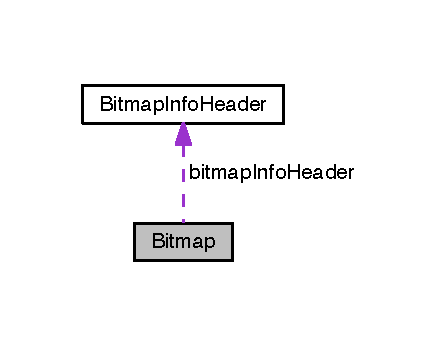
\includegraphics[width=210pt]{struct_bitmap__coll__graph}
\end{center}
\end{figure}
\subsection*{Data Fields}
\begin{DoxyCompactItemize}
\item 
\hypertarget{struct_bitmap_a7157ca7f3ce4be47481c472fafd89313}{}\label{struct_bitmap_a7157ca7f3ce4be47481c472fafd89313} 
\hyperlink{struct_bitmap_info_header}{Bitmap\+Info\+Header} {\bfseries bitmap\+Info\+Header}
\item 
\hypertarget{struct_bitmap_a586c4bcc42cf22a033e8f60f24f627f0}{}\label{struct_bitmap_a586c4bcc42cf22a033e8f60f24f627f0} 
unsigned char $\ast$ {\bfseries bitmap\+Data}
\item 
\hypertarget{struct_bitmap_a6150e0515f7202e2fb518f7206ed97dc}{}\label{struct_bitmap_a6150e0515f7202e2fb518f7206ed97dc} 
int {\bfseries x}
\item 
\hypertarget{struct_bitmap_a0a2f84ed7838f07779ae24c5a9086d33}{}\label{struct_bitmap_a0a2f84ed7838f07779ae24c5a9086d33} 
int {\bfseries y}
\end{DoxyCompactItemize}


\subsection{Detailed Description}
Represents a \hyperlink{struct_bitmap}{Bitmap}. 

The documentation for this struct was generated from the following file\+:\begin{DoxyCompactItemize}
\item 
bitmap.\+h\end{DoxyCompactItemize}

\hypertarget{struct_bitmap_file_header}{}\section{Bitmap\+File\+Header Struct Reference}
\label{struct_bitmap_file_header}\index{Bitmap\+File\+Header@{Bitmap\+File\+Header}}
\subsection*{Data Fields}
\begin{DoxyCompactItemize}
\item 
\hypertarget{struct_bitmap_file_header_aa929142c5ddf34cf0915c97a617a1a63}{}\label{struct_bitmap_file_header_aa929142c5ddf34cf0915c97a617a1a63} 
unsigned short {\bfseries type}
\item 
\hypertarget{struct_bitmap_file_header_aac913b3a1f6ef005d66bf7a84428773e}{}\label{struct_bitmap_file_header_aac913b3a1f6ef005d66bf7a84428773e} 
unsigned int {\bfseries size}
\item 
\hypertarget{struct_bitmap_file_header_a05d5cbcb44f437341bd9fa37d589aced}{}\label{struct_bitmap_file_header_a05d5cbcb44f437341bd9fa37d589aced} 
unsigned int {\bfseries reserved}
\item 
\hypertarget{struct_bitmap_file_header_a29b5297d3393519050e3126c4cb07c1c}{}\label{struct_bitmap_file_header_a29b5297d3393519050e3126c4cb07c1c} 
unsigned int {\bfseries offset}
\end{DoxyCompactItemize}


The documentation for this struct was generated from the following file\+:\begin{DoxyCompactItemize}
\item 
bitmap.\+h\end{DoxyCompactItemize}

\hypertarget{struct_bitmap_info_header}{}\section{Bitmap\+Info\+Header Struct Reference}
\label{struct_bitmap_info_header}\index{Bitmap\+Info\+Header@{Bitmap\+Info\+Header}}
\subsection*{Data Fields}
\begin{DoxyCompactItemize}
\item 
\hypertarget{struct_bitmap_info_header_aac913b3a1f6ef005d66bf7a84428773e}{}\label{struct_bitmap_info_header_aac913b3a1f6ef005d66bf7a84428773e} 
unsigned int {\bfseries size}
\item 
\hypertarget{struct_bitmap_info_header_a2474a5474cbff19523a51eb1de01cda4}{}\label{struct_bitmap_info_header_a2474a5474cbff19523a51eb1de01cda4} 
int {\bfseries width}
\item 
\hypertarget{struct_bitmap_info_header_ad12fc34ce789bce6c8a05d8a17138534}{}\label{struct_bitmap_info_header_ad12fc34ce789bce6c8a05d8a17138534} 
int {\bfseries height}
\item 
\hypertarget{struct_bitmap_info_header_a8c89d091e05544a82dc2398eed99634f}{}\label{struct_bitmap_info_header_a8c89d091e05544a82dc2398eed99634f} 
unsigned short {\bfseries planes}
\item 
\hypertarget{struct_bitmap_info_header_a47d1d4d776f8fd3bb0f7dbc3c5aeb534}{}\label{struct_bitmap_info_header_a47d1d4d776f8fd3bb0f7dbc3c5aeb534} 
unsigned short {\bfseries bits}
\item 
\hypertarget{struct_bitmap_info_header_ad180079f62b44e49ec672c9ef6e078b3}{}\label{struct_bitmap_info_header_ad180079f62b44e49ec672c9ef6e078b3} 
unsigned int {\bfseries compression}
\item 
\hypertarget{struct_bitmap_info_header_adcd57a0168319e747bc8099218d3822c}{}\label{struct_bitmap_info_header_adcd57a0168319e747bc8099218d3822c} 
unsigned int {\bfseries image\+Size}
\item 
\hypertarget{struct_bitmap_info_header_ac6eaeb4c0876cf6cd899f41fe3c25ff5}{}\label{struct_bitmap_info_header_ac6eaeb4c0876cf6cd899f41fe3c25ff5} 
int {\bfseries x\+Resolution}
\item 
\hypertarget{struct_bitmap_info_header_aa2f350dd0bda750656d5db5f5e37b2b3}{}\label{struct_bitmap_info_header_aa2f350dd0bda750656d5db5f5e37b2b3} 
int {\bfseries y\+Resolution}
\item 
\hypertarget{struct_bitmap_info_header_aed4506bad904845183194f199f1bdb98}{}\label{struct_bitmap_info_header_aed4506bad904845183194f199f1bdb98} 
unsigned int {\bfseries n\+Colors}
\item 
\hypertarget{struct_bitmap_info_header_a8f7abfbc446b12f385d2b42c3b4fd9b0}{}\label{struct_bitmap_info_header_a8f7abfbc446b12f385d2b42c3b4fd9b0} 
unsigned int {\bfseries important\+Colors}
\end{DoxyCompactItemize}


The documentation for this struct was generated from the following file\+:\begin{DoxyCompactItemize}
\item 
bitmap.\+h\end{DoxyCompactItemize}

\hypertarget{struct_bullet}{}\section{Bullet Struct Reference}
\label{struct_bullet}\index{Bullet@{Bullet}}


The \hyperlink{struct_bullet}{Bullet} \char`\"{}class\char`\"{} (Not really necessary, but good for code reading purposes)  




{\ttfamily \#include $<$bullet.\+h$>$}



Collaboration diagram for Bullet\+:
\nopagebreak
\begin{figure}[H]
\begin{center}
\leavevmode
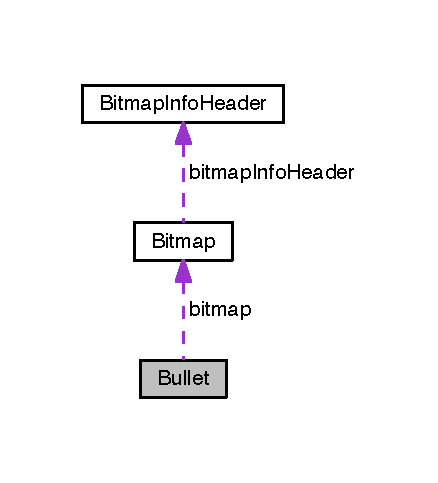
\includegraphics[width=210pt]{struct_bullet__coll__graph}
\end{center}
\end{figure}
\subsection*{Data Fields}
\begin{DoxyCompactItemize}
\item 
\hyperlink{struct_bitmap}{Bitmap} $\ast$ \hyperlink{struct_bullet_a00c870e2cedff0b231b1c8ad85019f66}{bitmap}
\end{DoxyCompactItemize}


\subsection{Detailed Description}
The \hyperlink{struct_bullet}{Bullet} \char`\"{}class\char`\"{} (Not really necessary, but good for code reading purposes) 

\subsection{Field Documentation}
\hypertarget{struct_bullet_a00c870e2cedff0b231b1c8ad85019f66}{}\label{struct_bullet_a00c870e2cedff0b231b1c8ad85019f66} 
\index{Bullet@{Bullet}!bitmap@{bitmap}}
\index{bitmap@{bitmap}!Bullet@{Bullet}}
\subsubsection{\texorpdfstring{bitmap}{bitmap}}
{\footnotesize\ttfamily \hyperlink{struct_bitmap}{Bitmap}$\ast$ bitmap}

Holds image of bullet (laser) and its position 

The documentation for this struct was generated from the following file\+:\begin{DoxyCompactItemize}
\item 
\hyperlink{bullet_8h}{bullet.\+h}\end{DoxyCompactItemize}

\hypertarget{struct_button}{}\section{Button Struct Reference}
\label{struct_button}\index{Button@{Button}}


The \hyperlink{struct_button}{Button} \char`\"{}class\char`\"{} (used for buttons present in main menu)  




{\ttfamily \#include $<$menu.\+h$>$}

\subsection*{Data Fields}
\begin{DoxyCompactItemize}
\item 
int \hyperlink{struct_button_af55497c668909df153bd9818cf765594}{xi}
\item 
int \hyperlink{struct_button_a525987ab72296fdd74c5bad7185fc0a4}{yi}
\item 
int \hyperlink{struct_button_a2474a5474cbff19523a51eb1de01cda4}{width}
\item 
int \hyperlink{struct_button_ad12fc34ce789bce6c8a05d8a17138534}{height}
\end{DoxyCompactItemize}


\subsection{Detailed Description}
The \hyperlink{struct_button}{Button} \char`\"{}class\char`\"{} (used for buttons present in main menu) 

\subsection{Field Documentation}
\hypertarget{struct_button_ad12fc34ce789bce6c8a05d8a17138534}{}\label{struct_button_ad12fc34ce789bce6c8a05d8a17138534} 
\index{Button@{Button}!height@{height}}
\index{height@{height}!Button@{Button}}
\subsubsection{\texorpdfstring{height}{height}}
{\footnotesize\ttfamily int height}

\hyperlink{struct_button}{Button}\textquotesingle{}s height \hypertarget{struct_button_a2474a5474cbff19523a51eb1de01cda4}{}\label{struct_button_a2474a5474cbff19523a51eb1de01cda4} 
\index{Button@{Button}!width@{width}}
\index{width@{width}!Button@{Button}}
\subsubsection{\texorpdfstring{width}{width}}
{\footnotesize\ttfamily int width}

\hyperlink{struct_button}{Button}\textquotesingle{}s width \hypertarget{struct_button_af55497c668909df153bd9818cf765594}{}\label{struct_button_af55497c668909df153bd9818cf765594} 
\index{Button@{Button}!xi@{xi}}
\index{xi@{xi}!Button@{Button}}
\subsubsection{\texorpdfstring{xi}{xi}}
{\footnotesize\ttfamily int xi}

\hyperlink{struct_button}{Button}\textquotesingle{}s top left corner x-\/coordinate \hypertarget{struct_button_a525987ab72296fdd74c5bad7185fc0a4}{}\label{struct_button_a525987ab72296fdd74c5bad7185fc0a4} 
\index{Button@{Button}!yi@{yi}}
\index{yi@{yi}!Button@{Button}}
\subsubsection{\texorpdfstring{yi}{yi}}
{\footnotesize\ttfamily int yi}

\hyperlink{struct_button}{Button}\textquotesingle{}s top left corner y-\/coordinate 

The documentation for this struct was generated from the following file\+:\begin{DoxyCompactItemize}
\item 
\hyperlink{menu_8h}{menu.\+h}\end{DoxyCompactItemize}

\hypertarget{struct_dispatcher}{}\section{Dispatcher Struct Reference}
\label{struct_dispatcher}\index{Dispatcher@{Dispatcher}}


The \hyperlink{struct_dispatcher}{Dispatcher} \char`\"{}class\char`\"{}.  




{\ttfamily \#include $<$dispatcher.\+h$>$}

\subsection*{Data Fields}
\begin{DoxyCompactItemize}
\item 
int \hyperlink{struct_dispatcher_a1d02e668b2cd1d4d633b562f437b8a4c}{irq\+\_\+timer}
\item 
int \hyperlink{struct_dispatcher_addcb3317227ee8bbc0304d8f3755cf21}{irq\+\_\+kbd}
\item 
int \hyperlink{struct_dispatcher_a899f4e59ee15429018efee9d38b533f1}{irq\+\_\+mouse}
\item 
int \hyperlink{struct_dispatcher_ac41513eff21d0a1e7c633f653c81eb0e}{irq\+\_\+rtc}
\item 
\hypertarget{struct_dispatcher_a9a27098ef2c3f4770fd8d4102a089c35}{}\label{struct_dispatcher_a9a27098ef2c3f4770fd8d4102a089c35} 
message {\bfseries msg}
\item 
\hypertarget{struct_dispatcher_ab9f863ebaa3805a6e366e055cd35626a}{}\label{struct_dispatcher_ab9f863ebaa3805a6e366e055cd35626a} 
int {\bfseries ipc\+\_\+status}
\item 
char $\ast$ \hyperlink{struct_dispatcher_a4be832ac49cb1384b79b9423028f1d54}{pwd}
\item 
\hypertarget{struct_dispatcher_ae3eef9568d40d16d1d14078d5bb9f069}{}\label{struct_dispatcher_ae3eef9568d40d16d1d14078d5bb9f069} 
\hyperlink{group__dispatcher_gafe31418b86c6754be94c8e79cfeed813}{dispatcherstate} {\bfseries state}
\end{DoxyCompactItemize}


\subsection{Detailed Description}
The \hyperlink{struct_dispatcher}{Dispatcher} \char`\"{}class\char`\"{}. 

\subsection{Field Documentation}
\hypertarget{struct_dispatcher_addcb3317227ee8bbc0304d8f3755cf21}{}\label{struct_dispatcher_addcb3317227ee8bbc0304d8f3755cf21} 
\index{Dispatcher@{Dispatcher}!irq\+\_\+kbd@{irq\+\_\+kbd}}
\index{irq\+\_\+kbd@{irq\+\_\+kbd}!Dispatcher@{Dispatcher}}
\subsubsection{\texorpdfstring{irq\+\_\+kbd}{irq\_kbd}}
{\footnotesize\ttfamily int irq\+\_\+kbd}

\hyperlink{struct_keyboard}{Keyboard}\textquotesingle{}s irq after respective interrupt subscription \hypertarget{struct_dispatcher_a899f4e59ee15429018efee9d38b533f1}{}\label{struct_dispatcher_a899f4e59ee15429018efee9d38b533f1} 
\index{Dispatcher@{Dispatcher}!irq\+\_\+mouse@{irq\+\_\+mouse}}
\index{irq\+\_\+mouse@{irq\+\_\+mouse}!Dispatcher@{Dispatcher}}
\subsubsection{\texorpdfstring{irq\+\_\+mouse}{irq\_mouse}}
{\footnotesize\ttfamily int irq\+\_\+mouse}

\hyperlink{struct_mouse}{Mouse}\textquotesingle{}s irq after respective interrupt subscription \hypertarget{struct_dispatcher_ac41513eff21d0a1e7c633f653c81eb0e}{}\label{struct_dispatcher_ac41513eff21d0a1e7c633f653c81eb0e} 
\index{Dispatcher@{Dispatcher}!irq\+\_\+rtc@{irq\+\_\+rtc}}
\index{irq\+\_\+rtc@{irq\+\_\+rtc}!Dispatcher@{Dispatcher}}
\subsubsection{\texorpdfstring{irq\+\_\+rtc}{irq\_rtc}}
{\footnotesize\ttfamily int irq\+\_\+rtc}

R\+TC\textquotesingle{}s irq after respective interrupt subscription \hypertarget{struct_dispatcher_a1d02e668b2cd1d4d633b562f437b8a4c}{}\label{struct_dispatcher_a1d02e668b2cd1d4d633b562f437b8a4c} 
\index{Dispatcher@{Dispatcher}!irq\+\_\+timer@{irq\+\_\+timer}}
\index{irq\+\_\+timer@{irq\+\_\+timer}!Dispatcher@{Dispatcher}}
\subsubsection{\texorpdfstring{irq\+\_\+timer}{irq\_timer}}
{\footnotesize\ttfamily int irq\+\_\+timer}

Timer0\textquotesingle{}s irq after respective interrupt subscription \hypertarget{struct_dispatcher_a4be832ac49cb1384b79b9423028f1d54}{}\label{struct_dispatcher_a4be832ac49cb1384b79b9423028f1d54} 
\index{Dispatcher@{Dispatcher}!pwd@{pwd}}
\index{pwd@{pwd}!Dispatcher@{Dispatcher}}
\subsubsection{\texorpdfstring{pwd}{pwd}}
{\footnotesize\ttfamily char$\ast$ pwd}

String that holds the session\textquotesingle{}s path -\/ value inserted by user as service run call\textquotesingle{}s argument 

The documentation for this struct was generated from the following file\+:\begin{DoxyCompactItemize}
\item 
\hyperlink{dispatcher_8h}{dispatcher.\+h}\end{DoxyCompactItemize}

\hypertarget{struct_game}{}\section{Game Struct Reference}
\label{struct_game}\index{Game@{Game}}


The \hyperlink{struct_game}{Game} \char`\"{}class\char`\"{}.  




{\ttfamily \#include $<$game.\+h$>$}



Collaboration diagram for Game\+:
\nopagebreak
\begin{figure}[H]
\begin{center}
\leavevmode
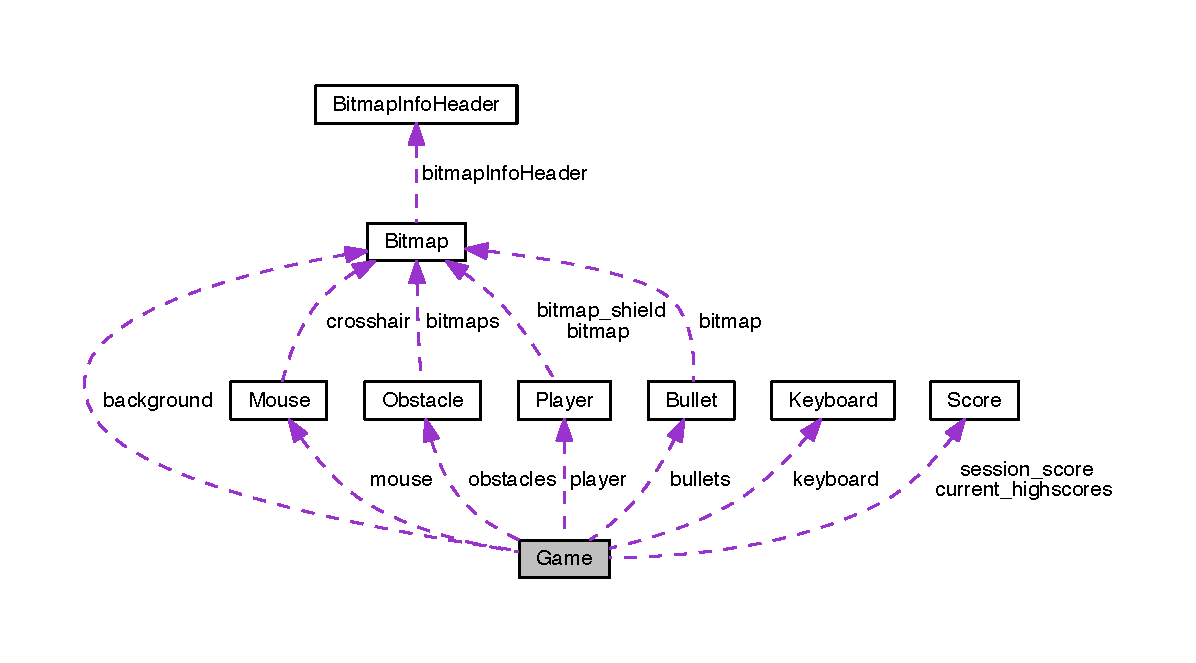
\includegraphics[width=350pt]{struct_game__coll__graph}
\end{center}
\end{figure}
\subsection*{Data Fields}
\begin{DoxyCompactItemize}
\item 
\hyperlink{struct_obstacle}{Obstacle} $\ast$$\ast$$\ast$ \hyperlink{struct_game_ab4a2d4a1db034550f0e6755c8417f00e}{obstacles}
\item 
\hyperlink{struct_mouse}{Mouse} $\ast$ \hyperlink{struct_game_a2514b83cbae6998a57eae74a24f6faf4}{mouse}
\item 
\hyperlink{struct_keyboard}{Keyboard} $\ast$ \hyperlink{struct_game_a945ceeb6236fbaf00dcdb7a0109f0d40}{keyboard}
\item 
\hyperlink{struct_bitmap}{Bitmap} $\ast$ \hyperlink{struct_game_a15de70574bc710486bf129a5c8f1634e}{background}
\item 
\hyperlink{struct_player}{Player} $\ast$ \hyperlink{struct_game_a96781128d3743da3d17e0fdd91afba7b}{player}
\item 
char $\ast$ \hyperlink{struct_game_a1820f1e9a26c0253b13be1df94052ca1}{secondary\+\_\+buffer}
\item 
\hyperlink{struct_bullet}{Bullet} $\ast$$\ast$ \hyperlink{struct_game_a6a95913dbac873584311bd479b43f911}{bullets}
\item 
\hyperlink{group__game_gab1e4078b5fa77cbf79de5e160f4cb261}{gamedrawstate} \hyperlink{struct_game_ab151fa4f58b0ddc30af7e501f6ba2ec3}{drawstate}
\item 
\hyperlink{group__game_ga33d4db650f69082296cc8c864c785e15}{gamestate} \hyperlink{struct_game_abb14911062a24c4178eb0f62fca2b925}{state}
\item 
\hyperlink{struct_score}{Score} $\ast$ \hyperlink{struct_game_ad7d780df0071261da7a401c839fa8a66}{session\+\_\+score}
\item 
\hyperlink{struct_score}{Score} $\ast$$\ast$ \hyperlink{struct_game_a544b8de55d5dc1667fad656b245d4a5a}{current\+\_\+highscores}
\item 
\hyperlink{group__game_ga74f568c551e9db616e8fae5ed65be48d}{scorenamestate} \hyperlink{struct_game_a49bcb1da4ed10a863fee60550febc40a}{namestate}
\item 
char \hyperlink{struct_game_a744d78025079ffc153f0be03356efdbe}{session\+\_\+name} \mbox{[}N\+A\+M\+E\+\_\+\+L\+E\+N\+G\+TH+1\mbox{]}
\end{DoxyCompactItemize}


\subsection{Detailed Description}
The \hyperlink{struct_game}{Game} \char`\"{}class\char`\"{}. 

\subsection{Field Documentation}
\hypertarget{struct_game_a15de70574bc710486bf129a5c8f1634e}{}\label{struct_game_a15de70574bc710486bf129a5c8f1634e} 
\index{Game@{Game}!background@{background}}
\index{background@{background}!Game@{Game}}
\subsubsection{\texorpdfstring{background}{background}}
{\footnotesize\ttfamily \hyperlink{struct_bitmap}{Bitmap}$\ast$ background}

The game background \hypertarget{struct_game_a6a95913dbac873584311bd479b43f911}{}\label{struct_game_a6a95913dbac873584311bd479b43f911} 
\index{Game@{Game}!bullets@{bullets}}
\index{bullets@{bullets}!Game@{Game}}
\subsubsection{\texorpdfstring{bullets}{bullets}}
{\footnotesize\ttfamily \hyperlink{struct_bullet}{Bullet}$\ast$$\ast$ bullets}

Array that holds information about current on-\/screen bullets (by other words, bullets shot by player) \hypertarget{struct_game_a544b8de55d5dc1667fad656b245d4a5a}{}\label{struct_game_a544b8de55d5dc1667fad656b245d4a5a} 
\index{Game@{Game}!current\+\_\+highscores@{current\+\_\+highscores}}
\index{current\+\_\+highscores@{current\+\_\+highscores}!Game@{Game}}
\subsubsection{\texorpdfstring{current\+\_\+highscores}{current\_highscores}}
{\footnotesize\ttfamily \hyperlink{struct_score}{Score}$\ast$$\ast$ current\+\_\+highscores}

Array that holds information about previous game sessions \hypertarget{struct_game_ab151fa4f58b0ddc30af7e501f6ba2ec3}{}\label{struct_game_ab151fa4f58b0ddc30af7e501f6ba2ec3} 
\index{Game@{Game}!drawstate@{drawstate}}
\index{drawstate@{drawstate}!Game@{Game}}
\subsubsection{\texorpdfstring{drawstate}{drawstate}}
{\footnotesize\ttfamily \hyperlink{group__game_gab1e4078b5fa77cbf79de5e160f4cb261}{gamedrawstate} drawstate}

Holds information about the game\textquotesingle{}s drawing state \hypertarget{struct_game_a945ceeb6236fbaf00dcdb7a0109f0d40}{}\label{struct_game_a945ceeb6236fbaf00dcdb7a0109f0d40} 
\index{Game@{Game}!keyboard@{keyboard}}
\index{keyboard@{keyboard}!Game@{Game}}
\subsubsection{\texorpdfstring{keyboard}{keyboard}}
{\footnotesize\ttfamily \hyperlink{struct_keyboard}{Keyboard}$\ast$ keyboard}

Holds information about keys pressed that will afect the game\textquotesingle{}s flow \hypertarget{struct_game_a2514b83cbae6998a57eae74a24f6faf4}{}\label{struct_game_a2514b83cbae6998a57eae74a24f6faf4} 
\index{Game@{Game}!mouse@{mouse}}
\index{mouse@{mouse}!Game@{Game}}
\subsubsection{\texorpdfstring{mouse}{mouse}}
{\footnotesize\ttfamily \hyperlink{struct_mouse}{Mouse}$\ast$ mouse}

Holds information about mouse movement to update the player\textquotesingle{}s position \hypertarget{struct_game_a49bcb1da4ed10a863fee60550febc40a}{}\label{struct_game_a49bcb1da4ed10a863fee60550febc40a} 
\index{Game@{Game}!namestate@{namestate}}
\index{namestate@{namestate}!Game@{Game}}
\subsubsection{\texorpdfstring{namestate}{namestate}}
{\footnotesize\ttfamily \hyperlink{group__game_ga74f568c551e9db616e8fae5ed65be48d}{scorenamestate} namestate}

Holds information about current session\textquotesingle{}s name letter receiving \hypertarget{struct_game_ab4a2d4a1db034550f0e6755c8417f00e}{}\label{struct_game_ab4a2d4a1db034550f0e6755c8417f00e} 
\index{Game@{Game}!obstacles@{obstacles}}
\index{obstacles@{obstacles}!Game@{Game}}
\subsubsection{\texorpdfstring{obstacles}{obstacles}}
{\footnotesize\ttfamily \hyperlink{struct_obstacle}{Obstacle}$\ast$$\ast$$\ast$ obstacles}

Matrix holding information about current on-\/screen obstacles \hypertarget{struct_game_a96781128d3743da3d17e0fdd91afba7b}{}\label{struct_game_a96781128d3743da3d17e0fdd91afba7b} 
\index{Game@{Game}!player@{player}}
\index{player@{player}!Game@{Game}}
\subsubsection{\texorpdfstring{player}{player}}
{\footnotesize\ttfamily \hyperlink{struct_player}{Player}$\ast$ player}

The main character \hypertarget{struct_game_a1820f1e9a26c0253b13be1df94052ca1}{}\label{struct_game_a1820f1e9a26c0253b13be1df94052ca1} 
\index{Game@{Game}!secondary\+\_\+buffer@{secondary\+\_\+buffer}}
\index{secondary\+\_\+buffer@{secondary\+\_\+buffer}!Game@{Game}}
\subsubsection{\texorpdfstring{secondary\+\_\+buffer}{secondary\_buffer}}
{\footnotesize\ttfamily char$\ast$ secondary\+\_\+buffer}

The double buffer used in the game \hypertarget{struct_game_a744d78025079ffc153f0be03356efdbe}{}\label{struct_game_a744d78025079ffc153f0be03356efdbe} 
\index{Game@{Game}!session\+\_\+name@{session\+\_\+name}}
\index{session\+\_\+name@{session\+\_\+name}!Game@{Game}}
\subsubsection{\texorpdfstring{session\+\_\+name}{session\_name}}
{\footnotesize\ttfamily char session\+\_\+name\mbox{[}N\+A\+M\+E\+\_\+\+L\+E\+N\+G\+TH+1\mbox{]}}

String that will store current session\textquotesingle{}s name (read from user input) \hypertarget{struct_game_ad7d780df0071261da7a401c839fa8a66}{}\label{struct_game_ad7d780df0071261da7a401c839fa8a66} 
\index{Game@{Game}!session\+\_\+score@{session\+\_\+score}}
\index{session\+\_\+score@{session\+\_\+score}!Game@{Game}}
\subsubsection{\texorpdfstring{session\+\_\+score}{session\_score}}
{\footnotesize\ttfamily \hyperlink{struct_score}{Score}$\ast$ session\+\_\+score}

Will hold information about the game session when it ends \hypertarget{struct_game_abb14911062a24c4178eb0f62fca2b925}{}\label{struct_game_abb14911062a24c4178eb0f62fca2b925} 
\index{Game@{Game}!state@{state}}
\index{state@{state}!Game@{Game}}
\subsubsection{\texorpdfstring{state}{state}}
{\footnotesize\ttfamily \hyperlink{group__game_ga33d4db650f69082296cc8c864c785e15}{gamestate} state}

Holds information about the game\textquotesingle{}s state 

The documentation for this struct was generated from the following file\+:\begin{DoxyCompactItemize}
\item 
\hyperlink{game_8h}{game.\+h}\end{DoxyCompactItemize}

\hypertarget{struct_keyboard}{}\section{Keyboard Struct Reference}
\label{struct_keyboard}\index{Keyboard@{Keyboard}}


The \hyperlink{struct_keyboard}{Keyboard} \char`\"{}class\char`\"{}.  




{\ttfamily \#include $<$keyboard.\+h$>$}

\subsection*{Data Fields}
\begin{DoxyCompactItemize}
\item 
unsigned long \hyperlink{struct_keyboard_a28472595f3d5303df45323230e37fc99}{scancode}
\item 
unsigned long \hyperlink{struct_keyboard_a47f04d0965fb400bb993629770de3f23}{scancode\+\_\+aux}
\item 
\hyperlink{group__keyboard_ga0b76c3eaf709ef57eecc834107a6d8cb}{scancodestate} \hyperlink{struct_keyboard_ae95dd0de5cee7e3f7148364eb9fa7b5b}{codestatus}
\end{DoxyCompactItemize}


\subsection{Detailed Description}
The \hyperlink{struct_keyboard}{Keyboard} \char`\"{}class\char`\"{}. 

\subsection{Field Documentation}
\hypertarget{struct_keyboard_ae95dd0de5cee7e3f7148364eb9fa7b5b}{}\label{struct_keyboard_ae95dd0de5cee7e3f7148364eb9fa7b5b} 
\index{Keyboard@{Keyboard}!codestatus@{codestatus}}
\index{codestatus@{codestatus}!Keyboard@{Keyboard}}
\subsubsection{\texorpdfstring{codestatus}{codestatus}}
{\footnotesize\ttfamily \hyperlink{group__keyboard_ga0b76c3eaf709ef57eecc834107a6d8cb}{scancodestate} codestatus}

Holds information about receiving the scancodes. Also serves as control \hypertarget{struct_keyboard_a28472595f3d5303df45323230e37fc99}{}\label{struct_keyboard_a28472595f3d5303df45323230e37fc99} 
\index{Keyboard@{Keyboard}!scancode@{scancode}}
\index{scancode@{scancode}!Keyboard@{Keyboard}}
\subsubsection{\texorpdfstring{scancode}{scancode}}
{\footnotesize\ttfamily unsigned long scancode}

Holds the current scancode \hypertarget{struct_keyboard_a47f04d0965fb400bb993629770de3f23}{}\label{struct_keyboard_a47f04d0965fb400bb993629770de3f23} 
\index{Keyboard@{Keyboard}!scancode\+\_\+aux@{scancode\+\_\+aux}}
\index{scancode\+\_\+aux@{scancode\+\_\+aux}!Keyboard@{Keyboard}}
\subsubsection{\texorpdfstring{scancode\+\_\+aux}{scancode\_aux}}
{\footnotesize\ttfamily unsigned long scancode\+\_\+aux}

Holds the first scancode byte in case of two byte scancodes 

The documentation for this struct was generated from the following file\+:\begin{DoxyCompactItemize}
\item 
\hyperlink{keyboard_8h}{keyboard.\+h}\end{DoxyCompactItemize}

\hypertarget{struct_menu}{}\section{Menu Struct Reference}
\label{struct_menu}\index{Menu@{Menu}}


The \hyperlink{struct_menu}{Menu} \char`\"{}class\char`\"{}.  




{\ttfamily \#include $<$menu.\+h$>$}

\subsection*{Data Fields}
\begin{DoxyCompactItemize}
\item 
\hyperlink{struct_button}{Button} $\ast$ \hyperlink{struct_menu_a17eeafa4c78aca8816c6aee85ce3a836}{play\+\_\+button}
\item 
\hyperlink{struct_button}{Button} $\ast$ \hyperlink{struct_menu_a173a61ec5be315a84389cc08d3852abe}{exit\+\_\+button}
\item 
\hyperlink{struct_mouse}{Mouse} $\ast$ \hyperlink{struct_menu_a2514b83cbae6998a57eae74a24f6faf4}{mouse}
\item 
\hyperlink{struct_keyboard}{Keyboard} $\ast$ \hyperlink{struct_menu_a945ceeb6236fbaf00dcdb7a0109f0d40}{keyboard}
\item 
\hyperlink{struct_bitmap}{Bitmap} $\ast$ \hyperlink{struct_menu_a15de70574bc710486bf129a5c8f1634e}{background}
\item 
char $\ast$ \hyperlink{struct_menu_a1820f1e9a26c0253b13be1df94052ca1}{secondary\+\_\+buffer}
\item 
\hyperlink{group__menu_ga187fcd377cc0b403aaec48d4cfdc559a}{menustate} \hyperlink{struct_menu_aa42946365311ec5aa5a3ab71b9c52968}{state}
\end{DoxyCompactItemize}


\subsection{Detailed Description}
The \hyperlink{struct_menu}{Menu} \char`\"{}class\char`\"{}. 

\subsection{Field Documentation}
\hypertarget{struct_menu_a15de70574bc710486bf129a5c8f1634e}{}\label{struct_menu_a15de70574bc710486bf129a5c8f1634e} 
\index{Menu@{Menu}!background@{background}}
\index{background@{background}!Menu@{Menu}}
\subsubsection{\texorpdfstring{background}{background}}
{\footnotesize\ttfamily \hyperlink{struct_bitmap}{Bitmap}$\ast$ background}

The menu background \hypertarget{struct_menu_a173a61ec5be315a84389cc08d3852abe}{}\label{struct_menu_a173a61ec5be315a84389cc08d3852abe} 
\index{Menu@{Menu}!exit\+\_\+button@{exit\+\_\+button}}
\index{exit\+\_\+button@{exit\+\_\+button}!Menu@{Menu}}
\subsubsection{\texorpdfstring{exit\+\_\+button}{exit\_button}}
{\footnotesize\ttfamily \hyperlink{struct_button}{Button}$\ast$ exit\+\_\+button}

Holds information about E\+X\+IT button \hypertarget{struct_menu_a945ceeb6236fbaf00dcdb7a0109f0d40}{}\label{struct_menu_a945ceeb6236fbaf00dcdb7a0109f0d40} 
\index{Menu@{Menu}!keyboard@{keyboard}}
\index{keyboard@{keyboard}!Menu@{Menu}}
\subsubsection{\texorpdfstring{keyboard}{keyboard}}
{\footnotesize\ttfamily \hyperlink{struct_keyboard}{Keyboard}$\ast$ keyboard}

\hyperlink{struct_keyboard}{Keyboard} to store scancodes read (all are ignored except E\+S\+C\+\_\+\+B\+R\+E\+AK) \hypertarget{struct_menu_a2514b83cbae6998a57eae74a24f6faf4}{}\label{struct_menu_a2514b83cbae6998a57eae74a24f6faf4} 
\index{Menu@{Menu}!mouse@{mouse}}
\index{mouse@{mouse}!Menu@{Menu}}
\subsubsection{\texorpdfstring{mouse}{mouse}}
{\footnotesize\ttfamily \hyperlink{struct_mouse}{Mouse}$\ast$ mouse}

\hyperlink{struct_mouse}{Mouse} to be shown and used to select and option \hypertarget{struct_menu_a17eeafa4c78aca8816c6aee85ce3a836}{}\label{struct_menu_a17eeafa4c78aca8816c6aee85ce3a836} 
\index{Menu@{Menu}!play\+\_\+button@{play\+\_\+button}}
\index{play\+\_\+button@{play\+\_\+button}!Menu@{Menu}}
\subsubsection{\texorpdfstring{play\+\_\+button}{play\_button}}
{\footnotesize\ttfamily \hyperlink{struct_button}{Button}$\ast$ play\+\_\+button}

Holds information about P\+L\+AY button \hypertarget{struct_menu_a1820f1e9a26c0253b13be1df94052ca1}{}\label{struct_menu_a1820f1e9a26c0253b13be1df94052ca1} 
\index{Menu@{Menu}!secondary\+\_\+buffer@{secondary\+\_\+buffer}}
\index{secondary\+\_\+buffer@{secondary\+\_\+buffer}!Menu@{Menu}}
\subsubsection{\texorpdfstring{secondary\+\_\+buffer}{secondary\_buffer}}
{\footnotesize\ttfamily char$\ast$ secondary\+\_\+buffer}

The double buffer used for the menu \hypertarget{struct_menu_aa42946365311ec5aa5a3ab71b9c52968}{}\label{struct_menu_aa42946365311ec5aa5a3ab71b9c52968} 
\index{Menu@{Menu}!state@{state}}
\index{state@{state}!Menu@{Menu}}
\subsubsection{\texorpdfstring{state}{state}}
{\footnotesize\ttfamily \hyperlink{group__menu_ga187fcd377cc0b403aaec48d4cfdc559a}{menustate} state}

The choosing options\textquotesingle{} state information 

The documentation for this struct was generated from the following file\+:\begin{DoxyCompactItemize}
\item 
\hyperlink{menu_8h}{menu.\+h}\end{DoxyCompactItemize}

\hypertarget{structmmap__t}{}\section{mmap\+\_\+t Struct Reference}
\label{structmmap__t}\index{mmap\+\_\+t@{mmap\+\_\+t}}


{\ttfamily \#include $<$lmlib.\+h$>$}

\subsection*{Data Fields}
\begin{DoxyCompactItemize}
\item 
phys\+\_\+bytes \hyperlink{group__lmlib_gab7a85fe0db943529016cf606e3a7167f}{phys}
\begin{DoxyCompactList}\small\item\em physical address \end{DoxyCompactList}\item 
void $\ast$ \hyperlink{group__lmlib_ga6a0ea2231d30f2b025e0c4b9f12dd6db}{virtual}
\begin{DoxyCompactList}\small\item\em virtual address \end{DoxyCompactList}\item 
unsigned long \hyperlink{group__lmlib_ga1e1268d164c38e4f8a4f4eb9058b0601}{size}
\begin{DoxyCompactList}\small\item\em size of memory region \end{DoxyCompactList}\end{DoxyCompactItemize}


\subsection{Detailed Description}
Struct that keeps info regarding the mapping of physical memory to virtual memory 

The documentation for this struct was generated from the following file\+:\begin{DoxyCompactItemize}
\item 
lmlib.\+h\end{DoxyCompactItemize}

\hypertarget{struct_mouse}{}\section{Mouse Struct Reference}
\label{struct_mouse}\index{Mouse@{Mouse}}


The \hyperlink{struct_mouse}{Mouse} \char`\"{}class\char`\"{}.  




{\ttfamily \#include $<$mouse.\+h$>$}



Collaboration diagram for Mouse\+:
\nopagebreak
\begin{figure}[H]
\begin{center}
\leavevmode
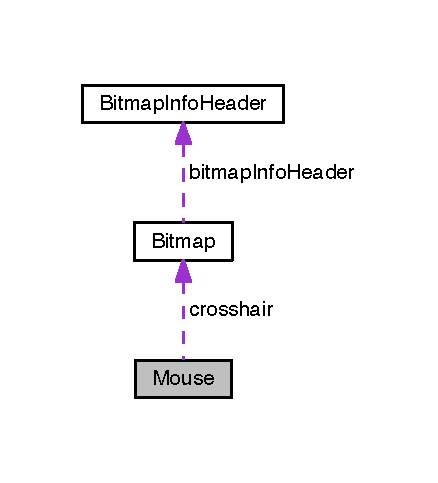
\includegraphics[width=210pt]{struct_mouse__coll__graph}
\end{center}
\end{figure}
\subsection*{Data Fields}
\begin{DoxyCompactItemize}
\item 
\hyperlink{group__mouse_gaab5a16f4c5c371d5048e7a729a8b45c7}{lbstate} \hyperlink{struct_mouse_a3460dc9908f5759debb0d94ccd939eb0}{left\+\_\+button\+\_\+state}
\item 
int \hyperlink{struct_mouse_a0fc78a583cf4573ff7df06591ac3b4ef}{left\+\_\+button\+\_\+was\+\_\+released}
\item 
\hyperlink{struct_bitmap}{Bitmap} $\ast$ \hyperlink{struct_mouse_a6d9b94480453acd797d61e51453ff026}{crosshair}
\item 
long \hyperlink{struct_mouse_a005ddb9e0f69d5f8ff8ba9811006637f}{packet\+\_\+byte}
\item 
unsigned int \hyperlink{struct_mouse_a593aab8c835cac0b2110f8d4e3f4124e}{byte\+ID}
\item 
unsigned char \hyperlink{struct_mouse_a1d1878244696a8be772aa71772c33f0a}{packet} \mbox{[}3\mbox{]}
\item 
\hyperlink{group__mouse_ga15fce23ec12347df2f9ef8c3366eb01d}{packetstate} \hyperlink{struct_mouse_a600d48813331aacf281603f33b7ce452}{packet\+\_\+state}
\end{DoxyCompactItemize}


\subsection{Detailed Description}
The \hyperlink{struct_mouse}{Mouse} \char`\"{}class\char`\"{}. 

\subsection{Field Documentation}
\hypertarget{struct_mouse_a593aab8c835cac0b2110f8d4e3f4124e}{}\label{struct_mouse_a593aab8c835cac0b2110f8d4e3f4124e} 
\index{Mouse@{Mouse}!byte\+ID@{byte\+ID}}
\index{byte\+ID@{byte\+ID}!Mouse@{Mouse}}
\subsubsection{\texorpdfstring{byte\+ID}{byteID}}
{\footnotesize\ttfamily unsigned int byte\+ID}

Holds position to store a packet\textquotesingle{}s byte in the array \hypertarget{struct_mouse_a6d9b94480453acd797d61e51453ff026}{}\label{struct_mouse_a6d9b94480453acd797d61e51453ff026} 
\index{Mouse@{Mouse}!crosshair@{crosshair}}
\index{crosshair@{crosshair}!Mouse@{Mouse}}
\subsubsection{\texorpdfstring{crosshair}{crosshair}}
{\footnotesize\ttfamily \hyperlink{struct_bitmap}{Bitmap}$\ast$ crosshair}

\hyperlink{struct_mouse}{Mouse}\textquotesingle{}s crosshair that will be drawn in menu screen \hypertarget{struct_mouse_a3460dc9908f5759debb0d94ccd939eb0}{}\label{struct_mouse_a3460dc9908f5759debb0d94ccd939eb0} 
\index{Mouse@{Mouse}!left\+\_\+button\+\_\+state@{left\+\_\+button\+\_\+state}}
\index{left\+\_\+button\+\_\+state@{left\+\_\+button\+\_\+state}!Mouse@{Mouse}}
\subsubsection{\texorpdfstring{left\+\_\+button\+\_\+state}{left\_button\_state}}
{\footnotesize\ttfamily \hyperlink{group__mouse_gaab5a16f4c5c371d5048e7a729a8b45c7}{lbstate} left\+\_\+button\+\_\+state}

Holds information about left button\textquotesingle{}s pressing \hypertarget{struct_mouse_a0fc78a583cf4573ff7df06591ac3b4ef}{}\label{struct_mouse_a0fc78a583cf4573ff7df06591ac3b4ef} 
\index{Mouse@{Mouse}!left\+\_\+button\+\_\+was\+\_\+released@{left\+\_\+button\+\_\+was\+\_\+released}}
\index{left\+\_\+button\+\_\+was\+\_\+released@{left\+\_\+button\+\_\+was\+\_\+released}!Mouse@{Mouse}}
\subsubsection{\texorpdfstring{left\+\_\+button\+\_\+was\+\_\+released}{left\_button\_was\_released}}
{\footnotesize\ttfamily int left\+\_\+button\+\_\+was\+\_\+released}

Holds information about left button being pressed. Non-\/zero when lbstate if R\+E\+L\+E\+A\+S\+ED and the previous one was P\+R\+E\+S\+S\+ED \hypertarget{struct_mouse_a1d1878244696a8be772aa71772c33f0a}{}\label{struct_mouse_a1d1878244696a8be772aa71772c33f0a} 
\index{Mouse@{Mouse}!packet@{packet}}
\index{packet@{packet}!Mouse@{Mouse}}
\subsubsection{\texorpdfstring{packet}{packet}}
{\footnotesize\ttfamily unsigned char packet\mbox{[}3\mbox{]}}

Current packet \hypertarget{struct_mouse_a005ddb9e0f69d5f8ff8ba9811006637f}{}\label{struct_mouse_a005ddb9e0f69d5f8ff8ba9811006637f} 
\index{Mouse@{Mouse}!packet\+\_\+byte@{packet\+\_\+byte}}
\index{packet\+\_\+byte@{packet\+\_\+byte}!Mouse@{Mouse}}
\subsubsection{\texorpdfstring{packet\+\_\+byte}{packet\_byte}}
{\footnotesize\ttfamily long packet\+\_\+byte}

Packets\textquotesingle{} bytes read from O\+U\+T\+\_\+\+B\+UF \hypertarget{struct_mouse_a600d48813331aacf281603f33b7ce452}{}\label{struct_mouse_a600d48813331aacf281603f33b7ce452} 
\index{Mouse@{Mouse}!packet\+\_\+state@{packet\+\_\+state}}
\index{packet\+\_\+state@{packet\+\_\+state}!Mouse@{Mouse}}
\subsubsection{\texorpdfstring{packet\+\_\+state}{packet\_state}}
{\footnotesize\ttfamily \hyperlink{group__mouse_ga15fce23ec12347df2f9ef8c3366eb01d}{packetstate} packet\+\_\+state}

Holds information about packet receiving. Also serves as control for update functions 

The documentation for this struct was generated from the following file\+:\begin{DoxyCompactItemize}
\item 
mouse.\+h\end{DoxyCompactItemize}

\hypertarget{struct_obstacle}{}\section{Obstacle Struct Reference}
\label{struct_obstacle}\index{Obstacle@{Obstacle}}


The \hyperlink{struct_obstacle}{Obstacle} \char`\"{}class\char`\"{}.  




{\ttfamily \#include $<$obstacle.\+h$>$}

\subsection*{Data Fields}
\begin{DoxyCompactItemize}
\item 
unsigned int \hyperlink{struct_obstacle_ab9d581d927d2e11f929ee02052f9eb58}{const\+\_\+lives}
\item 
unsigned int \hyperlink{struct_obstacle_a5b6f67c2402ab532f12e2422ddd2f5e4}{lives}
\item 
\hyperlink{struct_bitmap}{Bitmap} $\ast$ \hyperlink{struct_obstacle_ad89799fda86133fec366bb53373d93b8}{bitmaps} \mbox{[}M\+A\+X\+\_\+\+O\+B\+S\+T\+A\+C\+L\+E\+\_\+\+L\+I\+V\+ES\mbox{]}
\end{DoxyCompactItemize}


\subsection{Detailed Description}
The \hyperlink{struct_obstacle}{Obstacle} \char`\"{}class\char`\"{}. 

\subsection{Field Documentation}
\hypertarget{struct_obstacle_ad89799fda86133fec366bb53373d93b8}{}\label{struct_obstacle_ad89799fda86133fec366bb53373d93b8} 
\index{Obstacle@{Obstacle}!bitmaps@{bitmaps}}
\index{bitmaps@{bitmaps}!Obstacle@{Obstacle}}
\subsubsection{\texorpdfstring{bitmaps}{bitmaps}}
{\footnotesize\ttfamily \hyperlink{struct_bitmap}{Bitmap}$\ast$ bitmaps\mbox{[}M\+A\+X\+\_\+\+O\+B\+S\+T\+A\+C\+L\+E\+\_\+\+L\+I\+V\+ES\mbox{]}}

Holds possibilities of obstacle appearance. Different bitmap according to current number of lives \hypertarget{struct_obstacle_ab9d581d927d2e11f929ee02052f9eb58}{}\label{struct_obstacle_ab9d581d927d2e11f929ee02052f9eb58} 
\index{Obstacle@{Obstacle}!const\+\_\+lives@{const\+\_\+lives}}
\index{const\+\_\+lives@{const\+\_\+lives}!Obstacle@{Obstacle}}
\subsubsection{\texorpdfstring{const\+\_\+lives}{const\_lives}}
{\footnotesize\ttfamily unsigned int const\+\_\+lives}

Same initial value as \textquotesingle{}lives\textquotesingle{} but will never be modified (need value stored to increment player\textquotesingle{}s number of bullets later) \hypertarget{struct_obstacle_a5b6f67c2402ab532f12e2422ddd2f5e4}{}\label{struct_obstacle_a5b6f67c2402ab532f12e2422ddd2f5e4} 
\index{Obstacle@{Obstacle}!lives@{lives}}
\index{lives@{lives}!Obstacle@{Obstacle}}
\subsubsection{\texorpdfstring{lives}{lives}}
{\footnotesize\ttfamily unsigned int lives}

Holds obstacle\textquotesingle{}s current number of lives left 

The documentation for this struct was generated from the following file\+:\begin{DoxyCompactItemize}
\item 
\hyperlink{obstacle_8h}{obstacle.\+h}\end{DoxyCompactItemize}

\hypertarget{struct_player}{}\section{Player Struct Reference}
\label{struct_player}\index{Player@{Player}}


The \hyperlink{struct_player}{Player} \char`\"{}class\char`\"{}.  




{\ttfamily \#include $<$player.\+h$>$}



Collaboration diagram for Player\+:
\nopagebreak
\begin{figure}[H]
\begin{center}
\leavevmode
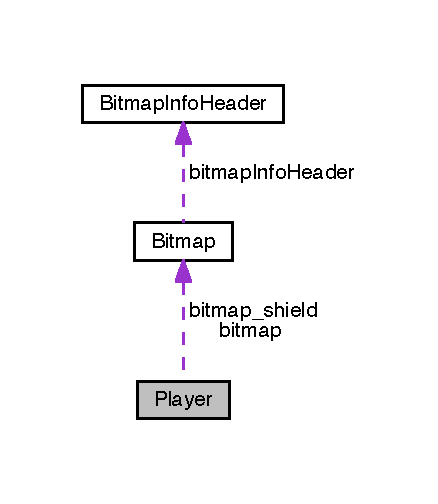
\includegraphics[width=210pt]{struct_player__coll__graph}
\end{center}
\end{figure}
\subsection*{Data Fields}
\begin{DoxyCompactItemize}
\item 
unsigned int \hyperlink{struct_player_a9ebf860aa3d67f9f3229afa365dbd2df}{score\+\_\+minutes}
\item 
unsigned int \hyperlink{struct_player_ac5b57794eda52960699e7304de9ed640}{score\+\_\+seconds}
\item 
int \hyperlink{struct_player_aa7c2d82515de928df40dec915c3ba081}{score\+\_\+aux}
\item 
unsigned int \hyperlink{struct_player_a391d726f640974bcd70eeba097a92ebf}{number\+\_\+of\+\_\+bullets}
\item 
unsigned int \hyperlink{struct_player_a0b2f5a7e6b082f9f828b559d165ac60f}{bonus\+\_\+timer}
\item 
\hyperlink{group__player_ga3ab4abfc8d967315be3486178b91d2d9}{bonusstate} \hyperlink{struct_player_ad071f1edf847f7378f6161c02ba70640}{bonus}
\item 
\hyperlink{struct_bitmap}{Bitmap} $\ast$ \hyperlink{struct_player_a00c870e2cedff0b231b1c8ad85019f66}{bitmap}
\item 
\hyperlink{struct_bitmap}{Bitmap} $\ast$ \hyperlink{struct_player_adb5f5a8861d7950622a415e122e4e6d7}{bitmap\+\_\+shield}
\end{DoxyCompactItemize}


\subsection{Detailed Description}
The \hyperlink{struct_player}{Player} \char`\"{}class\char`\"{}. 

\subsection{Field Documentation}
\hypertarget{struct_player_a00c870e2cedff0b231b1c8ad85019f66}{}\label{struct_player_a00c870e2cedff0b231b1c8ad85019f66} 
\index{Player@{Player}!bitmap@{bitmap}}
\index{bitmap@{bitmap}!Player@{Player}}
\subsubsection{\texorpdfstring{bitmap}{bitmap}}
{\footnotesize\ttfamily \hyperlink{struct_bitmap}{Bitmap}$\ast$ bitmap}

\hyperlink{struct_player}{Player}\textquotesingle{}s normal appearance \hypertarget{struct_player_adb5f5a8861d7950622a415e122e4e6d7}{}\label{struct_player_adb5f5a8861d7950622a415e122e4e6d7} 
\index{Player@{Player}!bitmap\+\_\+shield@{bitmap\+\_\+shield}}
\index{bitmap\+\_\+shield@{bitmap\+\_\+shield}!Player@{Player}}
\subsubsection{\texorpdfstring{bitmap\+\_\+shield}{bitmap\_shield}}
{\footnotesize\ttfamily \hyperlink{struct_bitmap}{Bitmap}$\ast$ bitmap\+\_\+shield}

\hyperlink{struct_player}{Player}\textquotesingle{}s appearance when invincibility bonus is on (has a rectangle shield around him) \hypertarget{struct_player_ad071f1edf847f7378f6161c02ba70640}{}\label{struct_player_ad071f1edf847f7378f6161c02ba70640} 
\index{Player@{Player}!bonus@{bonus}}
\index{bonus@{bonus}!Player@{Player}}
\subsubsection{\texorpdfstring{bonus}{bonus}}
{\footnotesize\ttfamily \hyperlink{group__player_ga3ab4abfc8d967315be3486178b91d2d9}{bonusstate} bonus}

Current bonus information \hypertarget{struct_player_a0b2f5a7e6b082f9f828b559d165ac60f}{}\label{struct_player_a0b2f5a7e6b082f9f828b559d165ac60f} 
\index{Player@{Player}!bonus\+\_\+timer@{bonus\+\_\+timer}}
\index{bonus\+\_\+timer@{bonus\+\_\+timer}!Player@{Player}}
\subsubsection{\texorpdfstring{bonus\+\_\+timer}{bonus\_timer}}
{\footnotesize\ttfamily unsigned int bonus\+\_\+timer}

Holds and controls bonus duration (initialized with B\+O\+N\+U\+S\+\_\+\+D\+U\+R\+A\+T\+I\+ON). Decremented until 0 every time score\+\_\+seconds is incremented \hypertarget{struct_player_a391d726f640974bcd70eeba097a92ebf}{}\label{struct_player_a391d726f640974bcd70eeba097a92ebf} 
\index{Player@{Player}!number\+\_\+of\+\_\+bullets@{number\+\_\+of\+\_\+bullets}}
\index{number\+\_\+of\+\_\+bullets@{number\+\_\+of\+\_\+bullets}!Player@{Player}}
\subsubsection{\texorpdfstring{number\+\_\+of\+\_\+bullets}{number\_of\_bullets}}
{\footnotesize\ttfamily unsigned int number\+\_\+of\+\_\+bullets}

Current number of bullets (lasers) player has left \hypertarget{struct_player_aa7c2d82515de928df40dec915c3ba081}{}\label{struct_player_aa7c2d82515de928df40dec915c3ba081} 
\index{Player@{Player}!score\+\_\+aux@{score\+\_\+aux}}
\index{score\+\_\+aux@{score\+\_\+aux}!Player@{Player}}
\subsubsection{\texorpdfstring{score\+\_\+aux}{score\_aux}}
{\footnotesize\ttfamily int score\+\_\+aux}

Counts timer0 interrupts to increment score at each second (really just counting time) \hypertarget{struct_player_a9ebf860aa3d67f9f3229afa365dbd2df}{}\label{struct_player_a9ebf860aa3d67f9f3229afa365dbd2df} 
\index{Player@{Player}!score\+\_\+minutes@{score\+\_\+minutes}}
\index{score\+\_\+minutes@{score\+\_\+minutes}!Player@{Player}}
\subsubsection{\texorpdfstring{score\+\_\+minutes}{score\_minutes}}
{\footnotesize\ttfamily unsigned int score\+\_\+minutes}

Current player\textquotesingle{}s minutes part of the score \hypertarget{struct_player_ac5b57794eda52960699e7304de9ed640}{}\label{struct_player_ac5b57794eda52960699e7304de9ed640} 
\index{Player@{Player}!score\+\_\+seconds@{score\+\_\+seconds}}
\index{score\+\_\+seconds@{score\+\_\+seconds}!Player@{Player}}
\subsubsection{\texorpdfstring{score\+\_\+seconds}{score\_seconds}}
{\footnotesize\ttfamily unsigned int score\+\_\+seconds}

Current player\textquotesingle{}s seconds part of the score 

The documentation for this struct was generated from the following file\+:\begin{DoxyCompactItemize}
\item 
\hyperlink{player_8h}{player.\+h}\end{DoxyCompactItemize}

\hypertarget{struct_score}{}\section{Score Struct Reference}
\label{struct_score}\index{Score@{Score}}


The \hyperlink{struct_score}{Score} \char`\"{}class\char`\"{}.  




{\ttfamily \#include $<$score.\+h$>$}

\subsection*{Data Fields}
\begin{DoxyCompactItemize}
\item 
unsigned int \hyperlink{struct_score_aa9526a2102bea713152f51e494eaaecb}{points\+\_\+minutes}
\item 
unsigned int \hyperlink{struct_score_a0eb13288839bf311a839235768f7e26c}{points\+\_\+seconds}
\item 
unsigned long \hyperlink{struct_score_ae9f072d0deb7c6120bb575d62e5bc5c3}{time} \mbox{[}D\+A\+T\+E\+\_\+\+L\+E\+N\+G\+TH\mbox{]}
\item 
unsigned long \hyperlink{struct_score_a8962e3d860b68ad109df42a45928b585}{date} \mbox{[}T\+I\+M\+E\+\_\+\+L\+E\+N\+G\+TH\mbox{]}
\item 
char \hyperlink{struct_score_a89a88337d531d6b5590602d97b5df8c0}{name} \mbox{[}N\+A\+M\+E\+\_\+\+L\+E\+N\+G\+TH\mbox{]}
\end{DoxyCompactItemize}


\subsection{Detailed Description}
The \hyperlink{struct_score}{Score} \char`\"{}class\char`\"{}. 

\subsection{Field Documentation}
\hypertarget{struct_score_a8962e3d860b68ad109df42a45928b585}{}\label{struct_score_a8962e3d860b68ad109df42a45928b585} 
\index{Score@{Score}!date@{date}}
\index{date@{date}!Score@{Score}}
\subsubsection{\texorpdfstring{date}{date}}
{\footnotesize\ttfamily unsigned long date\mbox{[}T\+I\+M\+E\+\_\+\+L\+E\+N\+G\+TH\mbox{]}}

The date when the score was obtained \hypertarget{struct_score_a89a88337d531d6b5590602d97b5df8c0}{}\label{struct_score_a89a88337d531d6b5590602d97b5df8c0} 
\index{Score@{Score}!name@{name}}
\index{name@{name}!Score@{Score}}
\subsubsection{\texorpdfstring{name}{name}}
{\footnotesize\ttfamily char name\mbox{[}N\+A\+M\+E\+\_\+\+L\+E\+N\+G\+TH\mbox{]}}

The name of the session when the score was obtained \hypertarget{struct_score_aa9526a2102bea713152f51e494eaaecb}{}\label{struct_score_aa9526a2102bea713152f51e494eaaecb} 
\index{Score@{Score}!points\+\_\+minutes@{points\+\_\+minutes}}
\index{points\+\_\+minutes@{points\+\_\+minutes}!Score@{Score}}
\subsubsection{\texorpdfstring{points\+\_\+minutes}{points\_minutes}}
{\footnotesize\ttfamily unsigned int points\+\_\+minutes}

The minutes part of a score \hypertarget{struct_score_a0eb13288839bf311a839235768f7e26c}{}\label{struct_score_a0eb13288839bf311a839235768f7e26c} 
\index{Score@{Score}!points\+\_\+seconds@{points\+\_\+seconds}}
\index{points\+\_\+seconds@{points\+\_\+seconds}!Score@{Score}}
\subsubsection{\texorpdfstring{points\+\_\+seconds}{points\_seconds}}
{\footnotesize\ttfamily unsigned int points\+\_\+seconds}

The seconds part of a score \hypertarget{struct_score_ae9f072d0deb7c6120bb575d62e5bc5c3}{}\label{struct_score_ae9f072d0deb7c6120bb575d62e5bc5c3} 
\index{Score@{Score}!time@{time}}
\index{time@{time}!Score@{Score}}
\subsubsection{\texorpdfstring{time}{time}}
{\footnotesize\ttfamily unsigned long time\mbox{[}D\+A\+T\+E\+\_\+\+L\+E\+N\+G\+TH\mbox{]}}

The time when the score was obtained 

The documentation for this struct was generated from the following file\+:\begin{DoxyCompactItemize}
\item 
\hyperlink{score_8h}{score.\+h}\end{DoxyCompactItemize}

\chapter{File Documentation}
\hypertarget{bullet_8h}{}\section{bullet.\+h File Reference}
\label{bullet_8h}\index{bullet.\+h@{bullet.\+h}}


Functions related with processing bullets (lasers) shot by player in-\/game.  


{\ttfamily \#include \char`\"{}player.\+h\char`\"{}}\newline
{\ttfamily \#include \char`\"{}bitmap.\+h\char`\"{}}\newline
{\ttfamily \#include \char`\"{}obstacle.\+h\char`\"{}}\newline
\subsection*{Data Structures}
\begin{DoxyCompactItemize}
\item 
struct \hyperlink{struct_bullet}{Bullet}
\begin{DoxyCompactList}\small\item\em The \hyperlink{struct_bullet}{Bullet} \char`\"{}class\char`\"{} (Not really necessary, but good for code reading purposes) \end{DoxyCompactList}\end{DoxyCompactItemize}
\subsection*{Macros}
\begin{DoxyCompactItemize}
\item 
\#define {\bfseries N\+\_\+\+B\+U\+L\+L\+E\+TS}~50
\item 
\#define {\bfseries M\+A\+X\+\_\+\+B\+U\+L\+L\+E\+T\+S\+\_\+\+O\+N\+\_\+\+S\+C\+R\+E\+EN}~10
\item 
\#define {\bfseries B\+U\+L\+L\+E\+T\+\_\+\+H\+E\+I\+G\+HT}~12
\item 
\#define {\bfseries B\+U\+L\+L\+E\+T\+\_\+\+O\+F\+F\+S\+ET}~37
\item 
\#define {\bfseries B\+U\+L\+L\+E\+T\+\_\+\+S\+P\+E\+ED}~3
\item 
\#define {\bfseries B\+U\+L\+L\+E\+T\+\_\+\+G\+A\+I\+N\+\_\+\+F\+A\+C\+T\+OR}~1
\end{DoxyCompactItemize}
\subsection*{Functions}
\begin{DoxyCompactItemize}
\item 
\hyperlink{struct_bullet}{Bullet} $\ast$ \hyperlink{group__bullet_gaf45d82f5138b8d8b424513cda1236282}{create\+\_\+bullet} (\hyperlink{struct_player}{Player} $\ast$player, int x, int y)
\begin{DoxyCompactList}\small\item\em Creates a new bullet at given position. \end{DoxyCompactList}\item 
int \hyperlink{group__bullet_ga821005fc4046140ee784eafbe32db07a}{bullet\+\_\+obstacle\+\_\+collision} (\hyperlink{struct_bullet}{Bullet} $\ast$bullet, \hyperlink{struct_obstacle}{Obstacle} $\ast$obstacle)
\begin{DoxyCompactList}\small\item\em Checks if there\textquotesingle{}s a collision between a certain bullet and a certain obstacle. \end{DoxyCompactList}\item 
int \hyperlink{group__bullet_ga18a96b8efbc45b8cbc1429f3660bae57}{update\+\_\+bullet} (\hyperlink{struct_bullet}{Bullet} $\ast$bullet)
\begin{DoxyCompactList}\small\item\em Updates a bullet\textquotesingle{}s position, checking if it goes off-\/screen in the process. \end{DoxyCompactList}\item 
void \hyperlink{group__bullet_ga9227bafd4863d90378dbcc48ebf68b93}{draw\+\_\+bullet} (\hyperlink{struct_bullet}{Bullet} $\ast$bullet, char $\ast$buffer)
\begin{DoxyCompactList}\small\item\em Draws a bullet at given buffer. \end{DoxyCompactList}\item 
void \hyperlink{group__bullet_ga715ca6e4284d7f977a09c8d141737e06}{delete\+\_\+bullet} (\hyperlink{struct_bullet}{Bullet} $\ast$bullet)
\begin{DoxyCompactList}\small\item\em Frees dynamically reserved memory and deletes bullet \textquotesingle{}object\textquotesingle{}. \end{DoxyCompactList}\end{DoxyCompactItemize}


\subsection{Detailed Description}
Functions related with processing bullets (lasers) shot by player in-\/game. 


\hypertarget{dispatcher_8h}{}\section{dispatcher.\+h File Reference}
\label{dispatcher_8h}\index{dispatcher.\+h@{dispatcher.\+h}}


Functions related with the program\textquotesingle{}s state and HW interruptions handling.  


{\ttfamily \#include $<$minix/syslib.\+h$>$}\newline
{\ttfamily \#include $<$minix/drivers.\+h$>$}\newline
{\ttfamily \#include $<$machine/int86.\+h$>$}\newline
{\ttfamily \#include $<$sys/mman.\+h$>$}\newline
{\ttfamily \#include $<$sys/types.\+h$>$}\newline
{\ttfamily \#include \char`\"{}menu.\+h\char`\"{}}\newline
{\ttfamily \#include \char`\"{}game.\+h\char`\"{}}\newline
Include dependency graph for dispatcher.\+h\+:
\nopagebreak
\begin{figure}[H]
\begin{center}
\leavevmode
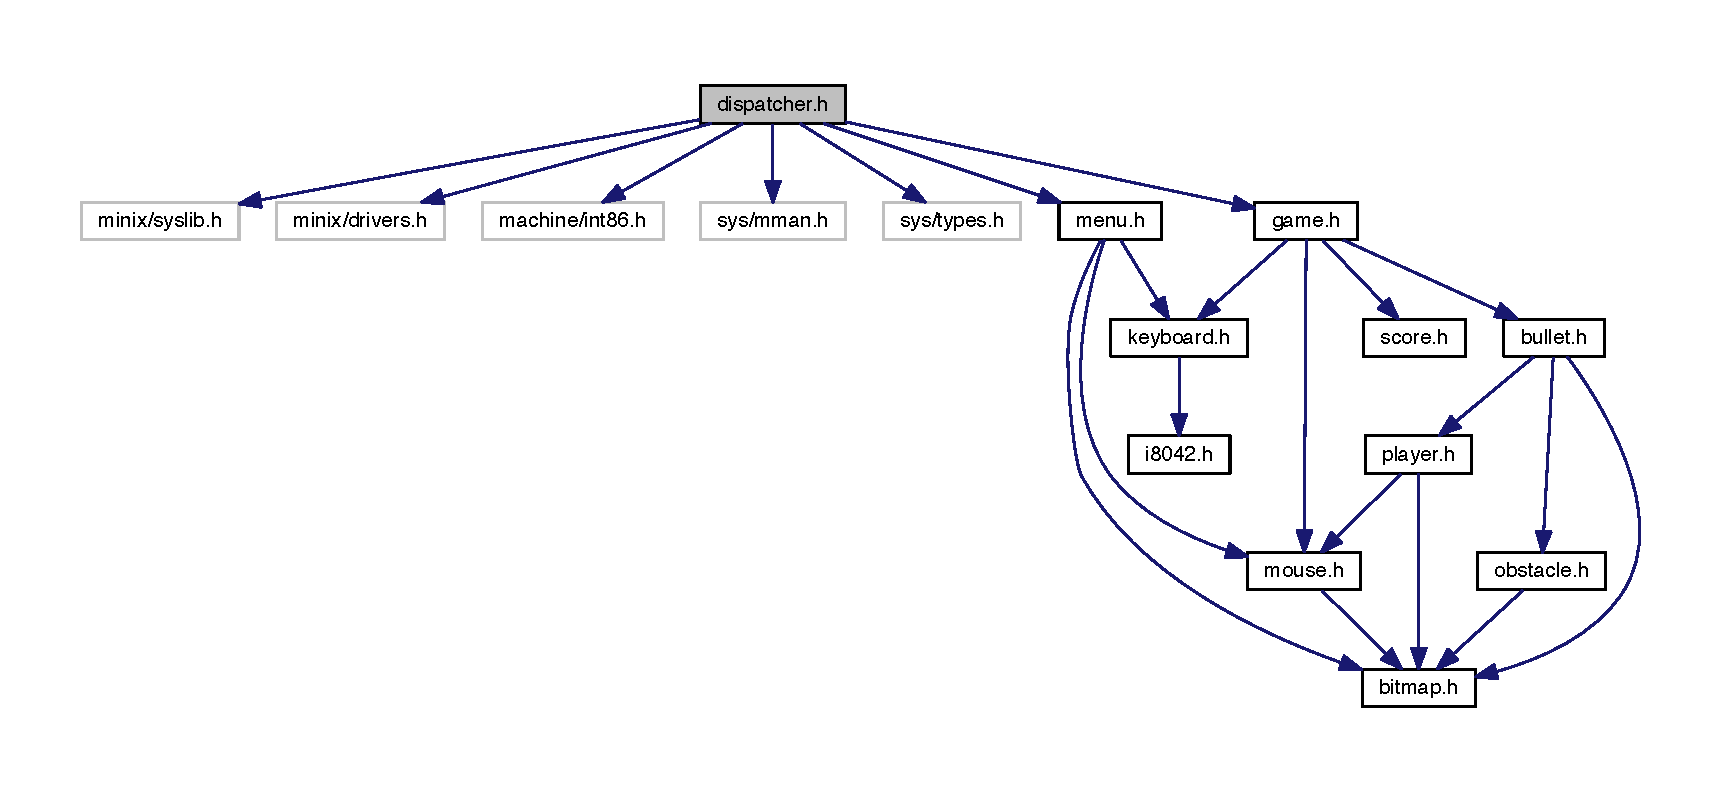
\includegraphics[width=350pt]{dispatcher_8h__incl}
\end{center}
\end{figure}
\subsection*{Data Structures}
\begin{DoxyCompactItemize}
\item 
struct \hyperlink{struct_dispatcher}{Dispatcher}
\begin{DoxyCompactList}\small\item\em The \hyperlink{struct_dispatcher}{Dispatcher} \char`\"{}class\char`\"{}. \end{DoxyCompactList}\end{DoxyCompactItemize}
\subsection*{Typedefs}
\begin{DoxyCompactItemize}
\item 
typedef enum \hyperlink{group__dispatcher_ga90e75071da8646d19ce0a3cd2926af3a}{dispatcherstate\+\_\+t} \hyperlink{group__dispatcher_gafe31418b86c6754be94c8e79cfeed813}{dispatcherstate}
\begin{DoxyCompactList}\small\item\em Possible \hyperlink{struct_dispatcher}{Dispatcher}\textquotesingle{}s states. \end{DoxyCompactList}\end{DoxyCompactItemize}
\subsection*{Enumerations}
\begin{DoxyCompactItemize}
\item 
\hypertarget{group__dispatcher_ga90e75071da8646d19ce0a3cd2926af3a}{}\label{group__dispatcher_ga90e75071da8646d19ce0a3cd2926af3a} 
enum \hyperlink{group__dispatcher_ga90e75071da8646d19ce0a3cd2926af3a}{dispatcherstate\+\_\+t} \{ {\bfseries M\+A\+I\+N\+\_\+\+M\+E\+NU}, 
{\bfseries G\+A\+ME}, 
{\bfseries E\+X\+I\+T\+\_\+\+P\+R\+O\+G\+R\+AM}
 \}\begin{DoxyCompactList}\small\item\em Possible \hyperlink{struct_dispatcher}{Dispatcher}\textquotesingle{}s states. \end{DoxyCompactList}
\end{DoxyCompactItemize}
\subsection*{Functions}
\begin{DoxyCompactItemize}
\item 
\hyperlink{struct_dispatcher}{Dispatcher} $\ast$ \hyperlink{group__dispatcher_ga806e2b40b340c9431427c77f94e859fa}{create\+\_\+dispatcher} (char $\ast$path)
\begin{DoxyCompactList}\small\item\em Subscribes to hardware peripherals and initializes \hyperlink{struct_dispatcher}{Dispatcher}\textquotesingle{}s members. Also initializes variable used to store the session\textquotesingle{}s path. \end{DoxyCompactList}\item 
void \hyperlink{group__dispatcher_ga4a58ba5ba48cbbaa0aad022b75685942}{delete\+\_\+dispatcher} (\hyperlink{struct_dispatcher}{Dispatcher} $\ast$dispatcher)
\begin{DoxyCompactList}\small\item\em Frees dynamically allocated memory by \hyperlink{struct_dispatcher}{Dispatcher}\textquotesingle{}s members. \end{DoxyCompactList}\item 
char $\ast$ \hyperlink{group__dispatcher_ga5ac2060f25333e39dcf8ea5a304b310f}{get\+\_\+pwd} ()
\begin{DoxyCompactList}\small\item\em Returns the repository\textquotesingle{}s parent directory path. \end{DoxyCompactList}\item 
void \hyperlink{group__dispatcher_ga2f999b67515a92fc53d29324552cd141}{interrupt\+\_\+handler} (\hyperlink{struct_dispatcher}{Dispatcher} $\ast$dispatcher)
\begin{DoxyCompactList}\small\item\em Initializes either game or menu based on dispatcher\textquotesingle{}s state. Includes driver receive loop that calls game specific functions to handle hardware interruptions, which loops until the dispatcher\textquotesingle{}s state changes. \end{DoxyCompactList}\item 
void \hyperlink{group__dispatcher_ga3b358623605878251bcfa528381cb15e}{state\+\_\+handler} (\hyperlink{struct_dispatcher}{Dispatcher} $\ast$dispatcher, \hyperlink{struct_menu}{Menu} $\ast$menu, \hyperlink{struct_game}{Game} $\ast$game)
\begin{DoxyCompactList}\small\item\em State handler to determine dispatcher\textquotesingle{}s next state, based on menu or game\textquotesingle{}s states. Also deletes either menu or game if the dispatcher\textquotesingle{}s state changes. \end{DoxyCompactList}\end{DoxyCompactItemize}


\subsection{Detailed Description}
Functions related with the program\textquotesingle{}s state and HW interruptions handling. 

Functions for outputing data to screen in graphics mode.
\hypertarget{game_8h}{}\section{game.\+h File Reference}
\label{game_8h}\index{game.\+h@{game.\+h}}


Functions related with processing the main game.  


{\ttfamily \#include \char`\"{}mouse.\+h\char`\"{}}\newline
{\ttfamily \#include \char`\"{}keyboard.\+h\char`\"{}}\newline
{\ttfamily \#include \char`\"{}score.\+h\char`\"{}}\newline
{\ttfamily \#include \char`\"{}bullet.\+h\char`\"{}}\newline
Include dependency graph for game.\+h\+:
\nopagebreak
\begin{figure}[H]
\begin{center}
\leavevmode
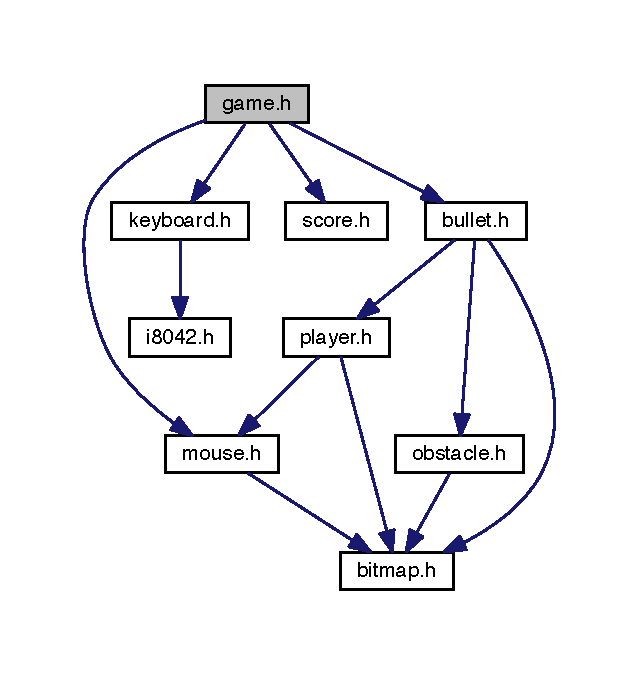
\includegraphics[width=306pt]{game_8h__incl}
\end{center}
\end{figure}
This graph shows which files directly or indirectly include this file\+:
\nopagebreak
\begin{figure}[H]
\begin{center}
\leavevmode
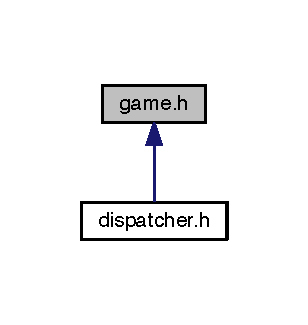
\includegraphics[width=148pt]{game_8h__dep__incl}
\end{center}
\end{figure}
\subsection*{Data Structures}
\begin{DoxyCompactItemize}
\item 
struct \hyperlink{struct_game}{Game}
\begin{DoxyCompactList}\small\item\em The \hyperlink{struct_game}{Game} \char`\"{}class\char`\"{}. \end{DoxyCompactList}\end{DoxyCompactItemize}
\subsection*{Macros}
\begin{DoxyCompactItemize}
\item 
\#define {\bfseries P\+L\+A\+Y\+E\+R\+\_\+\+N\+A\+M\+E\+\_\+\+X\+\_\+\+S\+T\+A\+RT}~300
\item 
\#define {\bfseries P\+L\+A\+Y\+E\+R\+\_\+\+N\+A\+M\+E\+\_\+\+Y\+\_\+\+S\+T\+A\+RT}~266
\item 
\#define {\bfseries P\+A\+U\+S\+E\+\_\+\+M\+E\+S\+S\+A\+G\+E\+\_\+X}~300
\item 
\#define {\bfseries P\+A\+U\+S\+E\+\_\+\+M\+E\+S\+S\+A\+G\+E\+\_\+Y}~264
\item 
\#define {\bfseries U\+N\+D\+E\+R\+S\+C\+O\+R\+E\+\_\+\+G\+AP}~67
\item 
\#define {\bfseries H\+I\+G\+H\+S\+C\+O\+R\+E\+\_\+\+N\+A\+M\+E\+\_\+X}~120
\item 
\#define {\bfseries H\+I\+G\+H\+S\+C\+O\+R\+E\+\_\+\+N\+A\+M\+E\+\_\+Y}~57
\end{DoxyCompactItemize}
\subsection*{Typedefs}
\begin{DoxyCompactItemize}
\item 
typedef enum \hyperlink{group__game_gaa3df7fce134ae5843a2bd6cdcd5796d0}{gamestate\+\_\+t} \hyperlink{group__game_ga33d4db650f69082296cc8c864c785e15}{gamestate}
\begin{DoxyCompactList}\small\item\em Possible game states. \end{DoxyCompactList}\item 
typedef enum \hyperlink{group__game_gab8e853703f9cb99b52ba53bcf16b5c4a}{scorenamestate\+\_\+t} \hyperlink{group__game_ga74f568c551e9db616e8fae5ed65be48d}{scorenamestate}
\begin{DoxyCompactList}\small\item\em Possible game session\textquotesingle{}s name receiving states. \end{DoxyCompactList}\item 
typedef enum \hyperlink{group__game_ga9984788ca86b30e008e68a755caeb998}{gamedrawstate\+\_\+t} \hyperlink{group__game_gab1e4078b5fa77cbf79de5e160f4cb261}{gamedrawstate}
\begin{DoxyCompactList}\small\item\em Possible game drawing states. \end{DoxyCompactList}\end{DoxyCompactItemize}
\subsection*{Enumerations}
\begin{DoxyCompactItemize}
\item 
\hypertarget{group__game_gaa3df7fce134ae5843a2bd6cdcd5796d0}{}\label{group__game_gaa3df7fce134ae5843a2bd6cdcd5796d0} 
enum \hyperlink{group__game_gaa3df7fce134ae5843a2bd6cdcd5796d0}{gamestate\+\_\+t} \{ {\bfseries G\+A\+M\+E\+\_\+\+R\+U\+N\+N\+I\+NG}, 
{\bfseries G\+A\+M\+E\+\_\+\+P\+A\+U\+S\+ED}, 
{\bfseries G\+A\+M\+E\+\_\+\+S\+C\+O\+RE}, 
{\bfseries G\+A\+M\+E\+\_\+\+O\+V\+ER}
 \}\begin{DoxyCompactList}\small\item\em Possible game states. \end{DoxyCompactList}
\item 
\hypertarget{group__game_gab8e853703f9cb99b52ba53bcf16b5c4a}{}\label{group__game_gab8e853703f9cb99b52ba53bcf16b5c4a} 
enum \hyperlink{group__game_gab8e853703f9cb99b52ba53bcf16b5c4a}{scorenamestate\+\_\+t} \{ \newline
{\bfseries F\+I\+R\+S\+T\+\_\+\+L\+E\+T\+T\+ER}, 
{\bfseries S\+E\+C\+O\+N\+D\+\_\+\+L\+E\+T\+T\+ER}, 
{\bfseries T\+H\+I\+R\+D\+\_\+\+L\+E\+T\+T\+ER}, 
{\bfseries F\+O\+U\+R\+T\+H\+\_\+\+L\+E\+T\+T\+ER}, 
\newline
{\bfseries N\+A\+M\+E\+\_\+\+R\+E\+C\+E\+I\+V\+ED}
 \}\begin{DoxyCompactList}\small\item\em Possible game session\textquotesingle{}s name receiving states. \end{DoxyCompactList}
\item 
\hypertarget{group__game_ga9984788ca86b30e008e68a755caeb998}{}\label{group__game_ga9984788ca86b30e008e68a755caeb998} 
enum \hyperlink{group__game_ga9984788ca86b30e008e68a755caeb998}{gamedrawstate\+\_\+t} \{ {\bfseries D\+O\+N\+T\+D\+R\+AW}, 
{\bfseries D\+R\+AW}
 \}\begin{DoxyCompactList}\small\item\em Possible game drawing states. \end{DoxyCompactList}
\end{DoxyCompactItemize}
\subsection*{Functions}
\begin{DoxyCompactItemize}
\item 
\hyperlink{struct_game}{Game} $\ast$ \hyperlink{group__game_gaabb10419dbd089ed1f572a817bea10ee}{create\+\_\+game} ()
\begin{DoxyCompactList}\small\item\em Creates a new game session. \end{DoxyCompactList}\item 
int \hyperlink{group__game_ga419536b6c803dd698c45680932477690}{determine\+\_\+index} (int bullet\+\_\+x)
\begin{DoxyCompactList}\small\item\em Calculates the index of the obstacle to test collision with (used for bullet-\/obstacle collisions) \end{DoxyCompactList}\item 
void \hyperlink{group__game_gaf0f9fdea8b3749557a89193e12153e1e}{update\+\_\+game\+\_\+running} (\hyperlink{struct_game}{Game} $\ast$game)
\begin{DoxyCompactList}\small\item\em Updates a game session that hasn\textquotesingle{}t finished yet. \end{DoxyCompactList}\item 
void \hyperlink{group__game_gaae19b3df5cdf51786306772dc362cc78}{game\+\_\+score\+\_\+event\+\_\+handler} (\hyperlink{struct_game}{Game} $\ast$game, char current\+\_\+key)
\begin{DoxyCompactList}\small\item\em Updates the current session\textquotesingle{}s name letter receiving state machine according to latest key received from user input. \end{DoxyCompactList}\item 
void \hyperlink{group__game_ga7fb225326dc8e9874c6ae3ac8b92e590}{update\+\_\+game\+\_\+score} (\hyperlink{struct_game}{Game} $\ast$game)
\begin{DoxyCompactList}\small\item\em Updates a game session that has finished (and therefore is on the final score screen) \end{DoxyCompactList}\item 
void \hyperlink{group__game_ga6d509d99fcf7deead2ccb896bfce5b78}{detect\+\_\+game\+\_\+end} (\hyperlink{struct_game}{Game} $\ast$game)
\begin{DoxyCompactList}\small\item\em Checks if a game has ended (if player got pushed off-\/screen by an obstacle). Updates the attribute gamestate if necessary. \end{DoxyCompactList}\item 
void \hyperlink{group__game_ga60f9b07b784e68d3c43cc63c54847e92}{update\+\_\+draw\+\_\+state} (\hyperlink{struct_game}{Game} $\ast$game)
\begin{DoxyCompactList}\small\item\em Every time it is called it flips the game\textquotesingle{}s attribute drawstate. Options are D\+O\+N\+T\+D\+R\+AW and D\+R\+AW (guarantees 30fps game) \end{DoxyCompactList}\item 
void \hyperlink{group__game_ga0e5a63798b2083168206005d4b9dcd83}{draw\+\_\+game} (\hyperlink{struct_game}{Game} $\ast$game)
\begin{DoxyCompactList}\small\item\em Copies frame stored in menu\textquotesingle{}s secondary buffer to the main buffer (video\+\_\+mem) \end{DoxyCompactList}\item 
int \hyperlink{group__game_gac31aaf764e55a4a6de1082340f7e5ed8}{add\+\_\+bullet\+\_\+shot} (\hyperlink{struct_game}{Game} $\ast$game, int x, int y)
\begin{DoxyCompactList}\small\item\em Tries to shoot a bullet from the player\textquotesingle{}s position. \end{DoxyCompactList}\item 
void \hyperlink{group__game_ga11217e4d270598c9ab99d632d090b942}{delete\+\_\+game} (\hyperlink{struct_game}{Game} $\ast$game)
\begin{DoxyCompactList}\small\item\em Frees dynamically reserved memory and deletes \textquotesingle{}object\textquotesingle{}. \end{DoxyCompactList}\end{DoxyCompactItemize}


\subsection{Detailed Description}
Functions related with processing the main game. 


\hypertarget{keyboard_8h}{}\section{keyboard.\+h File Reference}
\label{keyboard_8h}\index{keyboard.\+h@{keyboard.\+h}}


Functions related with processing the i8042\textquotesingle{}s keyboard.  


{\ttfamily \#include \char`\"{}i8042.\+h\char`\"{}}\newline
Include dependency graph for keyboard.\+h\+:
\nopagebreak
\begin{figure}[H]
\begin{center}
\leavevmode
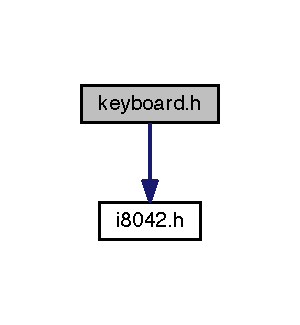
\includegraphics[width=144pt]{keyboard_8h__incl}
\end{center}
\end{figure}
This graph shows which files directly or indirectly include this file\+:
\nopagebreak
\begin{figure}[H]
\begin{center}
\leavevmode
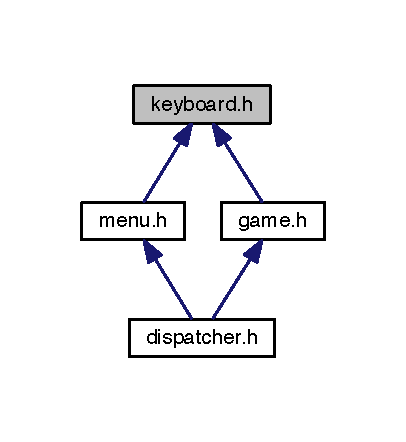
\includegraphics[width=195pt]{keyboard_8h__dep__incl}
\end{center}
\end{figure}
\subsection*{Data Structures}
\begin{DoxyCompactItemize}
\item 
struct \hyperlink{struct_keyboard}{Keyboard}
\begin{DoxyCompactList}\small\item\em The \hyperlink{struct_keyboard}{Keyboard} \char`\"{}class\char`\"{}. \end{DoxyCompactList}\end{DoxyCompactItemize}
\subsection*{Typedefs}
\begin{DoxyCompactItemize}
\item 
typedef enum \hyperlink{group__keyboard_gac25cb6c9d28679aed197b02d5885fcc2}{scancodestate\+\_\+t} \hyperlink{group__keyboard_ga0b76c3eaf709ef57eecc834107a6d8cb}{scancodestate}
\begin{DoxyCompactList}\small\item\em Possible scancode receiving states (there are scancodes with more than one byte) \end{DoxyCompactList}\end{DoxyCompactItemize}
\subsection*{Enumerations}
\begin{DoxyCompactItemize}
\item 
\hypertarget{group__keyboard_gac25cb6c9d28679aed197b02d5885fcc2}{}\label{group__keyboard_gac25cb6c9d28679aed197b02d5885fcc2} 
enum \hyperlink{group__keyboard_gac25cb6c9d28679aed197b02d5885fcc2}{scancodestate\+\_\+t} \{ {\bfseries R\+E\+A\+D\+\_\+\+A\+G\+A\+IN}, 
{\bfseries F\+U\+L\+L\+Y\+\_\+\+R\+E\+AD}
 \}\begin{DoxyCompactList}\small\item\em Possible scancode receiving states (there are scancodes with more than one byte) \end{DoxyCompactList}
\end{DoxyCompactItemize}
\subsection*{Functions}
\begin{DoxyCompactItemize}
\item 
int \hyperlink{group__keyboard_ga77e2ed8f53e0fae3f4005fa26c6d2692}{kbd\+\_\+subscribe\+\_\+int} ()
\begin{DoxyCompactList}\small\item\em Subscribes the i8042\textquotesingle{}s keyboard and enables its interrupts. \end{DoxyCompactList}\item 
int \hyperlink{group__keyboard_ga5bdf6cfb570c375192b0d87913b65c57}{kbd\+\_\+unsubscribe\+\_\+int} ()
\begin{DoxyCompactList}\small\item\em Unsubscribes the i8042\textquotesingle{}s keyboard\textquotesingle{}s interrupts. \end{DoxyCompactList}\item 
char \hyperlink{group__keyboard_ga837f1700d58c441769ddcfdae9792f13}{scancode\+\_\+to\+\_\+letter} (unsigned long code)
\begin{DoxyCompactList}\small\item\em Transforms breakcodes into the respective letter. \end{DoxyCompactList}\item 
\hyperlink{struct_keyboard}{Keyboard} $\ast$ \hyperlink{group__keyboard_ga12648eff06090040743ce7b51875afec}{create\+\_\+keyboard} ()
\begin{DoxyCompactList}\small\item\em Creates a new keyboard \textquotesingle{}object\textquotesingle{}. \end{DoxyCompactList}\item 
void \hyperlink{group__keyboard_ga97b5d5bf543266e60da0cc33c00aefad}{read\+\_\+scancode} (\hyperlink{struct_keyboard}{Keyboard} $\ast$keyboard)
\begin{DoxyCompactList}\small\item\em Reads a scancode (or part of it) from O\+U\+T\+\_\+\+B\+UF. Sets F\+U\+L\+L\+Y\+\_\+\+R\+E\+AD flag if full scancode is read. \end{DoxyCompactList}\item 
unsigned long \hyperlink{group__keyboard_ga4f6e388e1ad885350358a234aeed5be7}{read\+\_\+scancode\+\_\+asm} ()
\begin{DoxyCompactList}\small\item\em Externally defined -\/ read\+\_\+scancode\+\_\+asm. Reads a scancode (or part of it) from O\+U\+T\+\_\+\+B\+UF. Sets F\+U\+L\+L\+Y\+\_\+\+R\+E\+AD flag if full scancode is read. \end{DoxyCompactList}\item 
int \hyperlink{group__keyboard_gacd892a0b56fcd859cc2ed0bc17e32d7f}{full\+\_\+scancode\+\_\+received} (\hyperlink{struct_keyboard}{Keyboard} $\ast$keyboard)
\begin{DoxyCompactList}\small\item\em Checks if a full scancode has been read (through attribute codestatus) \end{DoxyCompactList}\item 
int \hyperlink{group__keyboard_gaa472854b178776886c9bf568945db9c6}{key\+\_\+detected} (\hyperlink{struct_keyboard}{Keyboard} $\ast$keyboard, unsigned long key)
\begin{DoxyCompactList}\small\item\em Checks if a given key has been pressed (or released, in case it\textquotesingle{}s a break code) \end{DoxyCompactList}\item 
void \hyperlink{group__keyboard_ga8cbe117a33793a5f88056d37164af0a8}{delete\+\_\+keyboard} (\hyperlink{struct_keyboard}{Keyboard} $\ast$keyboard)
\begin{DoxyCompactList}\small\item\em Frees dynamically reserved memory and deletes keyboard \textquotesingle{}object\textquotesingle{}. \end{DoxyCompactList}\end{DoxyCompactItemize}


\subsection{Detailed Description}
Functions related with processing the i8042\textquotesingle{}s keyboard. 


\hypertarget{menu_8h}{}\section{menu.\+h File Reference}
\label{menu_8h}\index{menu.\+h@{menu.\+h}}


Functions related with processing the program\textquotesingle{}s main menu.  


{\ttfamily \#include \char`\"{}bitmap.\+h\char`\"{}}\newline
{\ttfamily \#include \char`\"{}mouse.\+h\char`\"{}}\newline
{\ttfamily \#include \char`\"{}keyboard.\+h\char`\"{}}\newline
Include dependency graph for menu.\+h\+:
\nopagebreak
\begin{figure}[H]
\begin{center}
\leavevmode
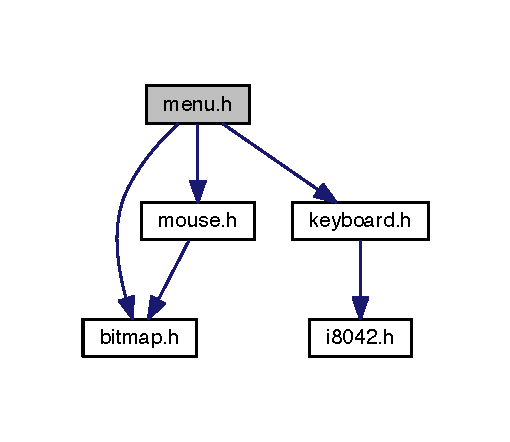
\includegraphics[width=245pt]{menu_8h__incl}
\end{center}
\end{figure}
This graph shows which files directly or indirectly include this file\+:
\nopagebreak
\begin{figure}[H]
\begin{center}
\leavevmode
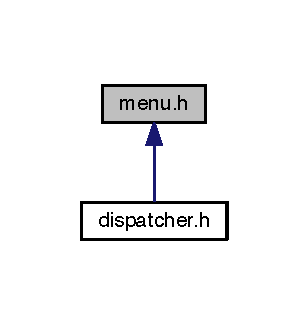
\includegraphics[width=148pt]{menu_8h__dep__incl}
\end{center}
\end{figure}
\subsection*{Data Structures}
\begin{DoxyCompactItemize}
\item 
struct \hyperlink{struct_button}{Button}
\begin{DoxyCompactList}\small\item\em The \hyperlink{struct_button}{Button} \char`\"{}class\char`\"{} (used for buttons present in main menu) \end{DoxyCompactList}\item 
struct \hyperlink{struct_menu}{Menu}
\begin{DoxyCompactList}\small\item\em The \hyperlink{struct_menu}{Menu} \char`\"{}class\char`\"{}. \end{DoxyCompactList}\end{DoxyCompactItemize}
\subsection*{Macros}
\begin{DoxyCompactItemize}
\item 
\#define {\bfseries P\+L\+A\+Y\+\_\+\+B\+U\+T\+T\+O\+N\+\_\+X}~300
\item 
\#define {\bfseries P\+L\+A\+Y\+\_\+\+B\+U\+T\+T\+O\+N\+\_\+Y}~280
\item 
\#define {\bfseries E\+X\+I\+T\+\_\+\+B\+U\+T\+T\+O\+N\+\_\+X}~300
\item 
\#define {\bfseries E\+X\+I\+T\+\_\+\+B\+U\+T\+T\+O\+N\+\_\+Y}~345
\item 
\#define {\bfseries B\+U\+T\+T\+O\+N\+\_\+\+W\+I\+D\+TH}~145
\item 
\#define {\bfseries B\+U\+T\+T\+O\+N\+\_\+\+H\+E\+I\+G\+HT}~50
\item 
\#define {\bfseries K\+B\+D\+\_\+\+U\+P\+D\+A\+TE}~0
\item 
\#define {\bfseries M\+O\+U\+S\+E\+\_\+\+U\+P\+D\+A\+TE}~1
\end{DoxyCompactItemize}
\subsection*{Typedefs}
\begin{DoxyCompactItemize}
\item 
typedef enum \hyperlink{group__menu_gafed699a28fc53900e4236f240af3b8c6}{menustate\+\_\+t} \hyperlink{group__menu_ga187fcd377cc0b403aaec48d4cfdc559a}{menustate}
\begin{DoxyCompactList}\small\item\em Possible \hyperlink{struct_menu}{Menu} choosing options\textquotesingle{} states. \end{DoxyCompactList}\end{DoxyCompactItemize}
\subsection*{Enumerations}
\begin{DoxyCompactItemize}
\item 
\hypertarget{group__menu_gafed699a28fc53900e4236f240af3b8c6}{}\label{group__menu_gafed699a28fc53900e4236f240af3b8c6} 
enum \hyperlink{group__menu_gafed699a28fc53900e4236f240af3b8c6}{menustate\+\_\+t} \{ {\bfseries N\+O\+T\+\_\+\+D\+O\+NE}, 
{\bfseries P\+L\+A\+Y\+\_\+\+C\+H\+O\+S\+EN}, 
{\bfseries E\+X\+I\+T\+\_\+\+C\+H\+O\+S\+EN}
 \}\begin{DoxyCompactList}\small\item\em Possible \hyperlink{struct_menu}{Menu} choosing options\textquotesingle{} states. \end{DoxyCompactList}
\end{DoxyCompactItemize}
\subsection*{Functions}
\begin{DoxyCompactItemize}
\item 
\hyperlink{struct_button}{Button} $\ast$ \hyperlink{group__menu_gaac1aca3c5e3ed5bccc82ccd7556138ed}{create\+\_\+button} (int x, int y, int width, int height)
\begin{DoxyCompactList}\small\item\em Creates a new button of given dimensions at given position. \end{DoxyCompactList}\item 
int \hyperlink{group__menu_ga137aca34f09e40a031dc463eab8d2050}{mouse\+\_\+on\+\_\+button} (\hyperlink{struct_button}{Button} $\ast$button, \hyperlink{struct_mouse}{Mouse} $\ast$mouse)
\begin{DoxyCompactList}\small\item\em Checks if given mouse is hovering over given button. \end{DoxyCompactList}\item 
void \hyperlink{group__menu_ga7fdafd18e6b0729fb26b435a54a072e7}{delete\+\_\+button} (\hyperlink{struct_button}{Button} $\ast$button)
\begin{DoxyCompactList}\small\item\em Frees dynamically reserved memory and deletes \textquotesingle{}object\textquotesingle{}. \end{DoxyCompactList}\item 
\hyperlink{struct_menu}{Menu} $\ast$ \hyperlink{group__menu_ga89bccdf2d8b12f81102d85e3b77d2505}{create\+\_\+menu} ()
\begin{DoxyCompactList}\small\item\em Creates a new main menu. \end{DoxyCompactList}\item 
void \hyperlink{group__menu_gabd716dc598e19aa573308e960c00cec1}{draw\+\_\+menu} (\hyperlink{struct_menu}{Menu} $\ast$menu)
\begin{DoxyCompactList}\small\item\em Copies frame stored in menu\textquotesingle{}s secondary buffer to the main buffer (video\+\_\+mem) \end{DoxyCompactList}\item 
void \hyperlink{group__menu_ga99bc2dfd43702a29bdcef45fea2f8391}{update\+\_\+menu} (\hyperlink{struct_menu}{Menu} $\ast$menu, int kbd\+\_\+or\+\_\+mouse)
\begin{DoxyCompactList}\small\item\em Updates a menu according to latest information received either from mouse or keyboard. \end{DoxyCompactList}\item 
void \hyperlink{group__menu_gacd664c37e26bab0e115dc3e1e3d3f3e2}{delete\+\_\+menu} (\hyperlink{struct_menu}{Menu} $\ast$menu)
\begin{DoxyCompactList}\small\item\em Frees dynamically reserved memory and deletes \textquotesingle{}object\textquotesingle{}. \end{DoxyCompactList}\end{DoxyCompactItemize}


\subsection{Detailed Description}
Functions related with processing the program\textquotesingle{}s main menu. 


\hypertarget{obstacle_8h}{}\section{obstacle.\+h File Reference}
\label{obstacle_8h}\index{obstacle.\+h@{obstacle.\+h}}


Functions related with processing the game\textquotesingle{}s obstacles.  


{\ttfamily \#include \char`\"{}bitmap.\+h\char`\"{}}\newline
Include dependency graph for obstacle.\+h\+:
\nopagebreak
\begin{figure}[H]
\begin{center}
\leavevmode
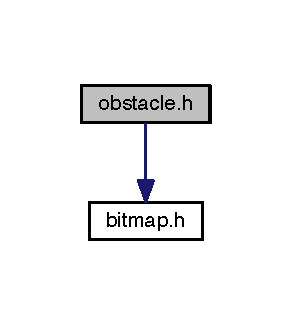
\includegraphics[width=140pt]{obstacle_8h__incl}
\end{center}
\end{figure}
This graph shows which files directly or indirectly include this file\+:
\nopagebreak
\begin{figure}[H]
\begin{center}
\leavevmode
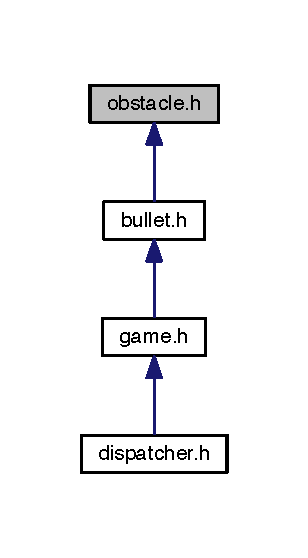
\includegraphics[width=148pt]{obstacle_8h__dep__incl}
\end{center}
\end{figure}
\subsection*{Data Structures}
\begin{DoxyCompactItemize}
\item 
struct \hyperlink{struct_obstacle}{Obstacle}
\begin{DoxyCompactList}\small\item\em The \hyperlink{struct_obstacle}{Obstacle} \char`\"{}class\char`\"{}. \end{DoxyCompactList}\end{DoxyCompactItemize}
\subsection*{Macros}
\begin{DoxyCompactItemize}
\item 
\#define {\bfseries O\+B\+S\+T\+A\+C\+L\+E\+\_\+\+S\+P\+E\+ED}~3
\item 
\#define {\bfseries O\+B\+S\+T\+A\+C\+L\+E\+\_\+\+W\+I\+D\+TH}~71
\item 
\#define {\bfseries O\+B\+S\+T\+A\+C\+L\+E\+\_\+\+H\+E\+I\+G\+HT}~66
\item 
\#define {\bfseries N\+\_\+\+O\+B\+S\+T\+A\+C\+L\+ES}~9
\item 
\#define {\bfseries E\+M\+P\+T\+Y\+\_\+\+F\+A\+C\+T\+OR}~2
\item 
\#define {\bfseries M\+A\+X\+\_\+\+O\+B\+S\+T\+A\+C\+L\+E\+\_\+\+L\+I\+V\+ES}~5
\item 
\#define {\bfseries N\+\_\+\+O\+B\+S\+T\+A\+C\+L\+E\+\_\+\+L\+I\+N\+ES}~2
\item 
\#define {\bfseries R\+A\+N\+D\+O\+M\+\_\+\+O\+B\+S\+T\+A\+C\+L\+E\+\_\+\+F\+A\+C\+T\+OR}~50
\end{DoxyCompactItemize}
\subsection*{Functions}
\begin{DoxyCompactItemize}
\item 
\hyperlink{struct_obstacle}{Obstacle} $\ast$ \hyperlink{group__obstacle_ga6624b86ef2320877c0935fb660f21dab}{create\+\_\+obstacle} (int x, int y)
\begin{DoxyCompactList}\small\item\em Creates a new obstacle with a random number of lives at given position. \end{DoxyCompactList}\item 
int \hyperlink{group__obstacle_gaf9a8875cab767c12b00817ed1b62ae4f}{update\+\_\+obstacle} (\hyperlink{struct_obstacle}{Obstacle} $\ast$obstacle)
\begin{DoxyCompactList}\small\item\em Updates an obstacle\textquotesingle{}s position, checking in the process if it goes off-\/screen. \end{DoxyCompactList}\item 
void \hyperlink{group__obstacle_ga9d4a8c6e21f6ef41233418d870b4a9c4}{draw\+\_\+obstacle} (\hyperlink{struct_obstacle}{Obstacle} $\ast$obstacle, char $\ast$buffer)
\begin{DoxyCompactList}\small\item\em Draws an obstacle at given buffer. \end{DoxyCompactList}\item 
int \hyperlink{group__obstacle_ga23812cfe6d34ed6fe00446f5e794a46e}{obstacle\+\_\+off\+\_\+screen} (\hyperlink{struct_obstacle}{Obstacle} $\ast$obstacle)
\begin{DoxyCompactList}\small\item\em Checks if a given obstacle\textquotesingle{}s top left corner is off-\/screen. \end{DoxyCompactList}\item 
void \hyperlink{group__obstacle_ga97f5becf2591663ecfe77e6da1f6aa2e}{delete\+\_\+obstacle} (\hyperlink{struct_obstacle}{Obstacle} $\ast$obstacle)
\begin{DoxyCompactList}\small\item\em Frees memory dynamically reserved for an obstacle and deletes it. \end{DoxyCompactList}\item 
void \hyperlink{group__obstacle_ga3c63dba1f24ebe9bef3e2dd2a5498006}{generate\+\_\+obstacle\+\_\+line} (\hyperlink{struct_obstacle}{Obstacle} $\ast$$\ast$obstacles, int line\+\_\+size, int line\+\_\+number)
\begin{DoxyCompactList}\small\item\em Generates a line of obstacles of specified size and position on the screen. \end{DoxyCompactList}\item 
void \hyperlink{group__obstacle_ga12e6975f62f13cef3f04d4014ac31242}{init\+\_\+current\+\_\+max\+\_\+lives} ()
\begin{DoxyCompactList}\small\item\em Initializes private global variable current\+\_\+max\+\_\+lives to 1. \end{DoxyCompactList}\item 
void \hyperlink{group__obstacle_gae8c5264a98edf73e34cc59b0d79ee5b8}{init\+\_\+current\+\_\+min\+\_\+lives} ()
\begin{DoxyCompactList}\small\item\em Initializes private global variable current\+\_\+min\+\_\+lives to 1. \end{DoxyCompactList}\item 
void \hyperlink{group__obstacle_ga6adaec54db6dd05a4bcdfb2abece7f98}{update\+\_\+lives\+\_\+boundaries} ()
\begin{DoxyCompactList}\small\item\em Updates the private global variables current\+\_\+min\+\_\+lives and current\+\_\+max\+\_\+lives to increase average number of lives of newly created obstacles. \end{DoxyCompactList}\item 
void \hyperlink{group__obstacle_gae44a832d131dcfc9009804066fd5fdf3}{delete\+\_\+obstacle\+\_\+line} (\hyperlink{struct_obstacle}{Obstacle} $\ast$$\ast$obstacles, int line\+\_\+size)
\begin{DoxyCompactList}\small\item\em Frees dynamically reserved memory and deletes entire line of obstacles. \end{DoxyCompactList}\end{DoxyCompactItemize}


\subsection{Detailed Description}
Functions related with processing the game\textquotesingle{}s obstacles. 


\hypertarget{player_8h}{}\section{player.\+h File Reference}
\label{player_8h}\index{player.\+h@{player.\+h}}


Functions related with processing the game\textquotesingle{}s character.  


{\ttfamily \#include \char`\"{}mouse.\+h\char`\"{}}\newline
{\ttfamily \#include \char`\"{}bitmap.\+h\char`\"{}}\newline
Include dependency graph for player.\+h\+:
\nopagebreak
\begin{figure}[H]
\begin{center}
\leavevmode
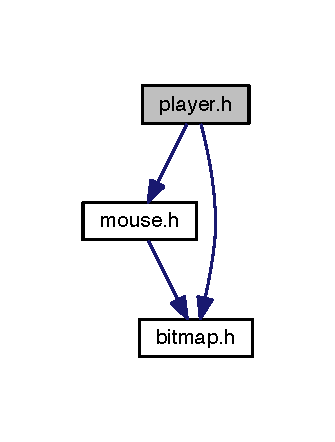
\includegraphics[width=161pt]{player_8h__incl}
\end{center}
\end{figure}
This graph shows which files directly or indirectly include this file\+:
\nopagebreak
\begin{figure}[H]
\begin{center}
\leavevmode
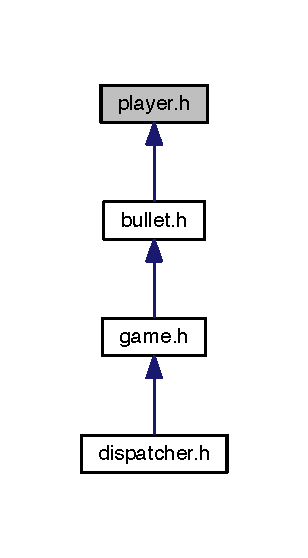
\includegraphics[width=148pt]{player_8h__dep__incl}
\end{center}
\end{figure}
\subsection*{Data Structures}
\begin{DoxyCompactItemize}
\item 
struct \hyperlink{struct_player}{Player}
\begin{DoxyCompactList}\small\item\em The \hyperlink{struct_player}{Player} \char`\"{}class\char`\"{}. \end{DoxyCompactList}\end{DoxyCompactItemize}
\subsection*{Macros}
\begin{DoxyCompactItemize}
\item 
\#define {\bfseries B\+L\+A\+CK}~0
\item 
\#define {\bfseries L\+E\+F\+T\+\_\+\+L\+I\+M\+IT}~75
\item 
\#define {\bfseries R\+I\+G\+H\+T\+\_\+\+L\+I\+M\+IT}~725
\item 
\#define {\bfseries N\+\_\+\+B\+U\+L\+L\+E\+TS}~50
\item 
\#define {\bfseries P\+L\+A\+Y\+E\+R\+\_\+\+S\+T\+A\+R\+T\+\_\+X}~75
\item 
\#define {\bfseries P\+L\+A\+Y\+E\+R\+\_\+\+S\+T\+A\+R\+T\+\_\+Y}~460
\item 
\#define {\bfseries P\+L\+A\+Y\+E\+R\+\_\+\+D\+E\+A\+T\+H\+\_\+\+T\+O\+L\+E\+R\+A\+N\+CE}~5
\item 
\#define {\bfseries N\+U\+M\+B\+E\+R\+\_\+\+O\+F\+\_\+\+B\+O\+N\+U\+S\+ES}~4
\item 
\#define {\bfseries B\+O\+N\+U\+S\+\_\+\+D\+U\+R\+A\+T\+I\+ON}~5
\item 
\#define {\bfseries B\+O\+N\+U\+S\+\_\+\+F\+R\+E\+Q\+U\+E\+N\+CY}~10
\end{DoxyCompactItemize}
\subsection*{Typedefs}
\begin{DoxyCompactItemize}
\item 
typedef enum \hyperlink{group__player_ga5bf5ff684470128c077a0e18436a6243}{bonusstate\+\_\+t} \hyperlink{group__player_ga3ab4abfc8d967315be3486178b91d2d9}{bonusstate}
\begin{DoxyCompactList}\small\item\em Possible bonuses (including no bonus) \end{DoxyCompactList}\end{DoxyCompactItemize}
\subsection*{Enumerations}
\begin{DoxyCompactItemize}
\item 
\hypertarget{group__player_ga5bf5ff684470128c077a0e18436a6243}{}\label{group__player_ga5bf5ff684470128c077a0e18436a6243} 
enum \hyperlink{group__player_ga5bf5ff684470128c077a0e18436a6243}{bonusstate\+\_\+t} \{ {\bfseries N\+O\+\_\+\+B\+O\+N\+US}, 
{\bfseries I\+N\+V\+I\+N\+C\+I\+B\+LE}, 
{\bfseries I\+N\+F\+I\+N\+I\+T\+E\+\_\+\+A\+M\+MO}, 
{\bfseries D\+O\+U\+B\+L\+E\+\_\+\+B\+U\+L\+L\+E\+TS}
 \}\begin{DoxyCompactList}\small\item\em Possible bonuses (including no bonus) \end{DoxyCompactList}
\end{DoxyCompactItemize}
\subsection*{Functions}
\begin{DoxyCompactItemize}
\item 
\hyperlink{struct_player}{Player} $\ast$ \hyperlink{group__player_ga37a8bafa3bd82b382ed0dc10b6a47bc6}{create\+\_\+player} ()
\begin{DoxyCompactList}\small\item\em Creates a new playable character when a new game session is initialized. \end{DoxyCompactList}\item 
void \hyperlink{group__player_ga4adc2e0586099acc41fc2a01f5fbd17b}{update\+\_\+player\+\_\+mouse} (\hyperlink{struct_player}{Player} $\ast$player, \hyperlink{struct_mouse}{Mouse} $\ast$mouse, char $\ast$buffer)
\begin{DoxyCompactList}\small\item\em Updates a player\textquotesingle{}s position based on latest mouse packet received. \end{DoxyCompactList}\item 
void \hyperlink{group__player_ga957878c48a3fb1afc3fcd55edf22c4dc}{update\+\_\+player\+\_\+collision} (\hyperlink{struct_player}{Player} $\ast$player, char $\ast$buffer)
\begin{DoxyCompactList}\small\item\em Updates a player\textquotesingle{}s position based on a possible collision with an obstacle. \end{DoxyCompactList}\item 
void \hyperlink{group__player_ga00245c5a0bd2c616f7bf886861cf0a59}{update\+\_\+number\+\_\+of\+\_\+bullets} (\hyperlink{struct_player}{Player} $\ast$player)
\begin{DoxyCompactList}\small\item\em Decrements a player\textquotesingle{}s number of bullets, unless he has an I\+N\+F\+I\+N\+I\+T\+E\+\_\+\+A\+M\+MO bonus activated. \end{DoxyCompactList}\item 
int \hyperlink{group__player_ga22a8eae795d9bddb858ac84d0e7371ed}{player\+\_\+has\+\_\+bullets} (\hyperlink{struct_player}{Player} $\ast$player)
\begin{DoxyCompactList}\small\item\em Checks if given player still has bullets (lasers) left. \end{DoxyCompactList}\item 
void \hyperlink{group__player_gafa760c994949e72cc685e338eca386e6}{generate\+\_\+bonus} (\hyperlink{struct_player}{Player} $\ast$player)
\begin{DoxyCompactList}\small\item\em Randomly generates a bonus and activates it immediately. \end{DoxyCompactList}\item 
void \hyperlink{group__player_ga2fa758d997a2b350ec55272a1cbe41eb}{update\+\_\+player\+\_\+score} (\hyperlink{struct_player}{Player} $\ast$player)
\begin{DoxyCompactList}\small\item\em Updates a player\textquotesingle{}s score. \end{DoxyCompactList}\item 
void \hyperlink{group__player_ga985b6963134729213326a13697741bd2}{update\+\_\+player\+\_\+bonus} (\hyperlink{struct_player}{Player} $\ast$player)
\begin{DoxyCompactList}\small\item\em Updates a player\textquotesingle{}s bonus duration (decrements it). If duration ends (reaches 0), bonus is removed. \end{DoxyCompactList}\item 
void \hyperlink{group__player_ga2c6f1674abdd49f8d225fa2c76b864de}{draw\+\_\+player} (\hyperlink{struct_player}{Player} $\ast$player, char $\ast$buffer)
\begin{DoxyCompactList}\small\item\em Draws a player at given buffer. \end{DoxyCompactList}\item 
void \hyperlink{group__player_ga9d6a1fdd44f008ff5eb4922118cce30a}{delete\+\_\+player} (\hyperlink{struct_player}{Player} $\ast$player)
\begin{DoxyCompactList}\small\item\em Frees dynamically reserved memory for a player and deletes the \textquotesingle{}object\textquotesingle{}. \end{DoxyCompactList}\end{DoxyCompactItemize}


\subsection{Detailed Description}
Functions related with processing the game\textquotesingle{}s character. 


\hypertarget{rtc_8h}{}\section{rtc.\+h File Reference}
\label{rtc_8h}\index{rtc.\+h@{rtc.\+h}}


Functions related with the usage of the PC\textquotesingle{}s Real Time Clock.  


\subsection*{Macros}
\begin{DoxyCompactItemize}
\item 
\hypertarget{rtc_8h_a61eabc8e73414cfe55910effa8bcc4ef}{}\label{rtc_8h_a61eabc8e73414cfe55910effa8bcc4ef} 
\#define {\bfseries C\+U\+R\+R\+E\+N\+T\+\_\+\+T\+I\+ME}~0
\item 
\hypertarget{rtc_8h_afdd5605d2281d188b0f997fb588d4420}{}\label{rtc_8h_afdd5605d2281d188b0f997fb588d4420} 
\#define {\bfseries C\+U\+R\+R\+E\+N\+T\+\_\+\+D\+A\+TE}~1
\end{DoxyCompactItemize}
\subsection*{Functions}
\begin{DoxyCompactItemize}
\item 
unsigned long $\ast$ \hyperlink{group__rtc_ga4ca5626e3ae7e8da1ad9183a7e6aa999}{rtc\+\_\+get} ()
\begin{DoxyCompactList}\small\item\em Externally defined function that returns an array containing the current date or time. \end{DoxyCompactList}\item 
int \hyperlink{group__rtc_gabd8de825e876e8ef94c64ac616f68a11}{rtc\+\_\+subscribe\+\_\+int} ()
\begin{DoxyCompactList}\small\item\em Subscribes Real Time Clock. \end{DoxyCompactList}\item 
int \hyperlink{group__rtc_gab8f17bf5280c908c8b199a90fefcc758}{rtc\+\_\+unsubscribe\+\_\+int} ()
\begin{DoxyCompactList}\small\item\em Unsubscribes Real Time Clock. \end{DoxyCompactList}\end{DoxyCompactItemize}
\subsection*{Variables}
\begin{DoxyCompactItemize}
\item 
unsigned long $\ast$ \hyperlink{group__rtc_gadc2ce94d90a689e95b0f88f7209bae2b}{result\+\_\+date}
\begin{DoxyCompactList}\small\item\em Externally declared array containing a date. \end{DoxyCompactList}\item 
unsigned long $\ast$ \hyperlink{group__rtc_ga3ee7a67468f7238ecea0abc3f33eb1ed}{result\+\_\+time}
\begin{DoxyCompactList}\small\item\em Externally declared array containing a time. \end{DoxyCompactList}\end{DoxyCompactItemize}


\subsection{Detailed Description}
Functions related with the usage of the PC\textquotesingle{}s Real Time Clock. 


\hypertarget{score_8h}{}\section{score.\+h File Reference}
\label{score_8h}\index{score.\+h@{score.\+h}}


Functions related with game score handling.  


\subsection*{Data Structures}
\begin{DoxyCompactItemize}
\item 
struct \hyperlink{struct_score}{Score}
\begin{DoxyCompactList}\small\item\em The \hyperlink{struct_score}{Score} \char`\"{}class\char`\"{}. \end{DoxyCompactList}\end{DoxyCompactItemize}
\subsection*{Macros}
\begin{DoxyCompactItemize}
\item 
\hypertarget{score_8h_afd9ee0dae9bd1ec89f11cda178c8b638}{}\label{score_8h_afd9ee0dae9bd1ec89f11cda178c8b638} 
\#define {\bfseries M\+A\+X\+\_\+\+S\+C\+O\+R\+E\+S\+\_\+\+R\+E\+AD}~15
\item 
\hypertarget{score_8h_af71324c57f05ff9e24bd384925dd6b17}{}\label{score_8h_af71324c57f05ff9e24bd384925dd6b17} 
\#define {\bfseries N\+A\+M\+E\+\_\+\+L\+E\+N\+G\+TH}~4
\item 
\hypertarget{score_8h_a94aa70086b6eee5f6cb297010fbaa78b}{}\label{score_8h_a94aa70086b6eee5f6cb297010fbaa78b} 
\#define {\bfseries D\+A\+T\+E\+\_\+\+L\+E\+N\+G\+TH}~3
\item 
\hypertarget{score_8h_a6680c1195df7df9797bdd639cb17e828}{}\label{score_8h_a6680c1195df7df9797bdd639cb17e828} 
\#define {\bfseries T\+I\+M\+E\+\_\+\+L\+E\+N\+G\+TH}~3
\item 
\hypertarget{score_8h_a6b348746b67879684605f536051cce97}{}\label{score_8h_a6b348746b67879684605f536051cce97} 
\#define {\bfseries M\+A\+X\+\_\+\+S\+C\+O\+R\+E\+S\+\_\+\+O\+N\+\_\+\+S\+C\+R\+E\+EN}~5
\item 
\hypertarget{score_8h_a2cccd6800509bae9bcbd792e4900cc7d}{}\label{score_8h_a2cccd6800509bae9bcbd792e4900cc7d} 
\#define {\bfseries S\+E\+S\+S\+I\+O\+N\+\_\+\+S\+C\+O\+R\+E\+\_\+\+X\+\_\+\+S\+T\+A\+RT}~332
\item 
\hypertarget{score_8h_a70d167f7f7fe8577db8525904a037167}{}\label{score_8h_a70d167f7f7fe8577db8525904a037167} 
\#define {\bfseries S\+E\+S\+S\+I\+O\+N\+\_\+\+S\+C\+O\+R\+E\+\_\+Y}~145
\item 
\hypertarget{score_8h_afb5ecdee202c538c9191d8e1e8b3699a}{}\label{score_8h_afb5ecdee202c538c9191d8e1e8b3699a} 
\#define {\bfseries H\+I\+G\+H\+S\+C\+O\+R\+E\+\_\+\+G\+AP}~30
\end{DoxyCompactItemize}
\subsection*{Functions}
\begin{DoxyCompactItemize}
\item 
\hyperlink{struct_score}{Score} $\ast$ \hyperlink{group__score_gac0781ace02ea3b0c0326eedcbe331017}{create\+\_\+score} (unsigned int new\+\_\+points\+\_\+minutes, unsigned int new\+\_\+points\+\_\+seconds, unsigned long $\ast$new\+\_\+time, unsigned long $\ast$new\+\_\+date, char $\ast$new\+\_\+name)
\begin{DoxyCompactList}\small\item\em Creates a new score from a recently finished game. \end{DoxyCompactList}\item 
void \hyperlink{group__score_gae35db4ff67df11b097733c7d9dd5a40f}{set\+\_\+score\+\_\+name} (\hyperlink{struct_score}{Score} $\ast$score, char $\ast$new\+\_\+name)
\begin{DoxyCompactList}\small\item\em Sets a score\textquotesingle{}s session name. \end{DoxyCompactList}\item 
void \hyperlink{group__score_ga00d69b4d67f70acd50560939535f2464}{draw\+\_\+score} (\hyperlink{struct_score}{Score} $\ast$score, int x, int y, char $\ast$buffer)
\begin{DoxyCompactList}\small\item\em Draws a score on given coordinates, at given buffer. \end{DoxyCompactList}\item 
void \hyperlink{group__score_ga2a08c01d91777c5e1166d04419dbb4c4}{draw\+\_\+scores} (\hyperlink{struct_score}{Score} $\ast$$\ast$scores, int x, int y, char $\ast$buffer)
\begin{DoxyCompactList}\small\item\em Draws an array of (high)scores on given coordinates, at given buffer. \end{DoxyCompactList}\item 
const char $\ast$ \hyperlink{group__score_ga7db0bd0fa660d164c6f16dcc3e45d709}{get\+\_\+scores\+\_\+file} ()
\begin{DoxyCompactList}\small\item\em Provides absolute path of highscores text file (file must be in proj/src) \end{DoxyCompactList}\item 
void \hyperlink{group__score_gafda13bf491b8895de5356e2e8e9e0006}{write\+\_\+score\+\_\+to\+\_\+file} (\hyperlink{struct_score}{Score} $\ast$score)
\begin{DoxyCompactList}\small\item\em Writes a score to the highscores text file (appended to existing ones) \end{DoxyCompactList}\item 
\hyperlink{struct_score}{Score} $\ast$$\ast$ \hyperlink{group__score_ga24850c38550bc5c6d3df0df15306a583}{read\+\_\+scores\+\_\+from\+\_\+file} ()
\begin{DoxyCompactList}\small\item\em Reads current scores saved in highscores text file. \end{DoxyCompactList}\item 
int \hyperlink{group__score_ga987e3955c36619ffa125c50620c85000}{comp\+\_\+score} (const void $\ast$s1, const void $\ast$s2)
\begin{DoxyCompactList}\small\item\em Compares two scores by their total score in seconds (used in qsort to sort highscores array) \end{DoxyCompactList}\item 
void \hyperlink{group__score_ga579c3c56eea0c910d596054bb9802d8c}{delete\+\_\+score} (\hyperlink{struct_score}{Score} $\ast$score)
\begin{DoxyCompactList}\small\item\em Frees memory dynamically reserved for a score. \end{DoxyCompactList}\end{DoxyCompactItemize}


\subsection{Detailed Description}
Functions related with game score handling. 


\hypertarget{timer_8h}{}\section{timer.\+h File Reference}
\label{timer_8h}\index{timer.\+h@{timer.\+h}}


Functions for using the i8254 timer0.  


\subsection*{Functions}
\begin{DoxyCompactItemize}
\item 
int \hyperlink{group__timer_ga4c5d9f47323eda494cfd826f6d62eec9}{timer\+\_\+subscribe\+\_\+int} (void)
\begin{DoxyCompactList}\small\item\em Subscribes and enables Timer 0 interrupts. \end{DoxyCompactList}\item 
int \hyperlink{group__timer_gab9eea51549744bca5c5c923b388bb4ee}{timer\+\_\+unsubscribe\+\_\+int} ()
\begin{DoxyCompactList}\small\item\em Unsubscribes Timer 0 interrupts. \end{DoxyCompactList}\end{DoxyCompactItemize}


\subsection{Detailed Description}
Functions for using the i8254 timer0. 


\hypertarget{utils_8h}{}\section{utils.\+h File Reference}
\label{utils_8h}\index{utils.\+h@{utils.\+h}}


General functions to aid the program flow.  


This graph shows which files directly or indirectly include this file\+:
\nopagebreak
\begin{figure}[H]
\begin{center}
\leavevmode
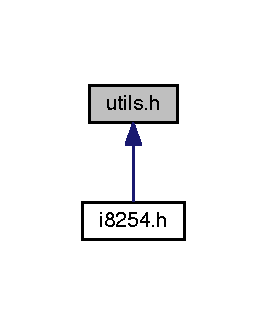
\includegraphics[width=128pt]{utils_8h__dep__incl}
\end{center}
\end{figure}
\subsection*{Macros}
\begin{DoxyCompactItemize}
\item 
\#define {\bfseries B\+IT}(n)~(0x01$<$$<$(n))
\item 
\#define {\bfseries T\+W\+O\+S\+C\+O\+M\+P\+L\+E\+M\+E\+NT}(N)~(short)(0xff00 $\vert$ N)
\item 
\#define {\bfseries A\+B\+S\+\_\+\+V\+A\+L\+UE}(X)~(X $<$ 0 ? -\/X \+: X)
\item 
\#define {\bfseries B\+C\+D\+\_\+\+L\+SD}(X)~(X \& 0x0000000\+F)
\item 
\#define {\bfseries G\+A\+M\+E\+\_\+\+N\+U\+M\+B\+E\+R\+\_\+\+W\+I\+D\+TH}~16
\item 
\#define {\bfseries S\+C\+O\+R\+E\+\_\+\+B\+I\+T\+M\+A\+P\+\_\+\+W\+I\+D\+TH}~30
\item 
\#define {\bfseries S\+C\+O\+R\+E\+\_\+\+B\+I\+T\+M\+A\+P\+\_\+\+H\+E\+I\+G\+HT}~30
\end{DoxyCompactItemize}
\subsection*{Functions}
\begin{DoxyCompactItemize}
\item 
const char $\ast$ \hyperlink{group__utils_gacd89c22fdefa32a68bfff93637677a38}{full\+Path} (const char $\ast$filename)
\begin{DoxyCompactList}\small\item\em Transforms an image filename into its absolute path. \end{DoxyCompactList}\item 
void \hyperlink{group__utils_ga1d3f15b906cf55d88a42ff86d9035978}{draw\+\_\+game\+\_\+number} (int number, int x, int y, char $\ast$buffer)
\begin{DoxyCompactList}\small\item\em Draws a 2 digit number (always) in given coordinates, at given buffer. \end{DoxyCompactList}\item 
char $\ast$ \hyperlink{group__utils_gac1f5ea8c8660adf99729789da39cf9ce}{number\+\_\+to\+\_\+string} (int number)
\begin{DoxyCompactList}\small\item\em Transforms a number into its respective english word and adds .bmp extension to it. \end{DoxyCompactList}\item 
void \hyperlink{group__utils_ga6c6627d0ed2f743fc34057524d37296f}{draw\+\_\+score\+\_\+number} (int number, int x, int y, char $\ast$buffer)
\begin{DoxyCompactList}\small\item\em Draws a 2 digit number (always) in given coordinates, at given buffer. \end{DoxyCompactList}\item 
void \hyperlink{group__utils_ga7f8f4adbdf567fe397208152fec35363}{draw\+\_\+colon} (int x, int y, char $\ast$buffer)
\begin{DoxyCompactList}\small\item\em Draws the character \textquotesingle{}\+:\textquotesingle{} on given coordinates, at given buffer (used to draw time) \end{DoxyCompactList}\item 
void \hyperlink{group__utils_ga189285abfa4707506b6d32a68639c755}{draw\+\_\+slash} (int x, int y, char $\ast$buffer)
\begin{DoxyCompactList}\small\item\em Draws the character \textquotesingle{}/\textquotesingle{} on given coordinates, at given buffer (used to draw date) \end{DoxyCompactList}\item 
void \hyperlink{group__utils_gac2e1e0cd9b6bedcac9364250a05ea853}{draw\+\_\+letter} (char letter, int x, int y, char $\ast$buffer)
\begin{DoxyCompactList}\small\item\em Draws a letter of the english alphabet on given coordinates, at given buffer. \end{DoxyCompactList}\item 
unsigned long \hyperlink{group__utils_ga85d2356c3023fbcaa278695aa20bd2b4}{bcd\+\_\+to\+\_\+binary} (unsigned long number\+\_\+in\+\_\+bcd)
\begin{DoxyCompactList}\small\item\em Converts a number in B\+CD to its binary representation. \end{DoxyCompactList}\item 
unsigned long $\ast$ \hyperlink{group__utils_ga9eb356657a418586720db2f80c1ef2b6}{bcd\+\_\+to\+\_\+binary\+\_\+array} (unsigned long $\ast$base, int size)
\begin{DoxyCompactList}\small\item\em Converts an array of numbers in B\+CD to their binary representation. \end{DoxyCompactList}\item 
int \hyperlink{group__utils_ga3bebfa53ca8923b1d684663aa409b286}{start\+\_\+graphic\+\_\+mode} ()
\begin{DoxyCompactList}\small\item\em Initializes graphic mode in mode 0x114 (800x600, 2 bytes per pixel) \end{DoxyCompactList}\item 
int \hyperlink{group__utils_ga65cd2418a6137ab0b6a403e25b098fcf}{exit\+\_\+graphic\+\_\+mode} ()
\begin{DoxyCompactList}\small\item\em Returns to M\+I\+N\+IX\textquotesingle{}s default text mode. \end{DoxyCompactList}\end{DoxyCompactItemize}


\subsection{Detailed Description}
General functions to aid the program flow. 


%--- End generated contents ---

% Index
\backmatter
\newpage
\phantomsection
\clearemptydoublepage
\addcontentsline{toc}{chapter}{Index}
\printindex

\end{document}
